%Mathdocs. MG changed some things, see end of document. This is the master copy, altered on 8/28/2022 for tkzEuclide
\documentclass[addpoints]{amsart} 
%\documentclass{tglat2e}%%   tglat calls the Class of our Journal.
\parskip 5pt
\textwidth 5.5in
%\linespread{1.2}
%\hoffset-.8truein
%\vsize10truein
%For large fonts, use \tiny, \scriptsize, \footnotesize, \Large, \LARGE, \huge, \Huge.

%\usepackage{gensymb} %for degree symbol
\usepackage{pgf, tikz} %8/26/22 I put in the pgf for Euclide
%\usepackage{tikzsymbols} %for emoticons! Call with \Smiley, \Sadey, \Neutrey, and put [2.0] to make it twice as big. see lists.
\usepackage{tikz-cd} %Commutative Diagrams. Use \[\begin{tikzcd} .. \end{tikzcd}\] You can make: A \arrow[hook]{r} & B
\usetikzlibrary{angles,arrows.meta,automata,backgrounds,calc,decorations.markings,decorations.pathreplacing,intersections,patterns,positioning,quotes} %For background figures, use \begin{scope}[on background layer] ... \end{scope}
\usetikzlibrary{shapes} %For polygon nodes, see http://www.texample.net/tikz/examples/node-shapes/
\usepgflibrary{shapes.geometric}
\usepackage{tkz-euclide} 
%Needed to resolve conflict between tkz-euclide and thmtools, see https://tex.stackexchange.com/questions/456029/thmtools-and-tkz-euclide-conflict
%\usetkzobj{all}
%\usepackage{thmtools}
\usepackage{etoolbox}
\usepackage{url}
\usepackage{hyperref}


\usepackage{mdframed} %\begin{mdframed}[backgroundcolor=green!10,linewidth=1pt] makes a colored box around an enumerate, etc.
\usepackage{pgfplots}
\pgfplotsset{width=10cm,compat=1.9}
\usepackage[export]{adjustbox}
\usepackage{caption}
\usepackage{subcaption}
\usepackage{wrapfig}
%See sharelatex.com
\usepackage{graphicx}
\usepackage{mathtools}  %This allows the \begin{bmatrix*} environment, and a [r] [l], or [c] which aligns the entries!
%See sharelatex.com
\usepackage{amsthm,thmtools} %This allows boxed theorem-like environments, see \declaretheorem as below
%I removed this 8/26/2022 trying to fix euclide, as I heard there was a conflict.
\usepackage{relsize} %for a cup product $\mathsmaller\cup$

\usepackage{fdsymbol} %Or {mnsymbol}
%\usepackage{amssymb, latexsym, amsmath} %is what we had before fdsymbol%, makeidx}
%\makeindex

\usepackage{amsmath,systeme} %this is for systems of equations. 
%You use \begin{equation*}\systeme{<put in system, separating equations with a comma>}\end{equation*}. 
%If you want to get rid of the delimiter, use \sysdelim..\systeme{ } instead.

\usepackage{fancyhdr} %headers and footers. On the document, put \pagestyle{fancy} before begin{document}, then use \rhead{Cal Poly}, \chead{\bf Math 241}, \lhead{Brussel}. Or, \fancyhead[L]{Math 483/560}, \fancyhead[R]{bbbbbbbbbbbbbbbbbb}, \fancyhead[C]{Structure}, then \begin{document}\thispagestyle{fancy} <- If you want the first page as well.

%FONTS:
\usepackage{courier}
%call it up with \texttt.  It gives an equally spaced courier font.
\input ArtNouvc.fd
\newcommand*\initfamily{\usefont{U}{ArtNouvc}{xl}{n}} %Fancy all caps. Call it with {\initfamily <text>}
\input Starburst.fd
\newcommand*\starinitfamily{\usefont{U}{Starburst}{xl}{n}}

\usepackage[all,cmtip]{xy}
%See website http://en.wikibooks.org/wiki/LaTeX/Creating_Graphics#XY-pic
%http://www.tug.org/pracjourn/2006-4/blaga/blaga.pdf

\usepackage{enumerate}
%Follow the usual \begin{enumerate} with [I] for roman numerals, and [(a)] for alphabetic symbols.
\usepackage{mdwlist}

%I blocked this when I put in tikz, because of a color clash.
%\usepackage[usenames, dvipsnames]{color}
%See website http://people.oregonstate.edu/~peterseb/tex/samples/color-package.html for
%a list of the many color options.  Or, http://en.wikibooks.org/wiki/LaTeX/Colors
%To invoke, use {\color{red}<text>}
%To make a new color, use \definecolor{orange}{rgb}{1,0.5,0}  Here rgb is red green blue.

%%%%% from Asher
\usepackage{mathrsfs} %nice script font
%%% UV - changes in header: %'d \usepackage{mathabx}, \def\divides, \def\notdivides.
%\usepackage{mathabx} % get \notdivides

\usepackage[OT2,T1]{fontenc}
\DeclareSymbolFont{cyrletters}{OT2}{wncyr}{m}{n}
\DeclareMathSymbol{\Sha}{\mathalpha}{cyrletters}{"58}



\theoremstyle{plain}
\newtheorem{Theorem}[subsubsection]{Theorem}
\newtheorem{Lemma}[subsubsection]{Lemma}
\newtheorem{Corollary}[subsubsection]{Corollary}
\newtheorem{Proposition}[subsubsection]{Proposition}
\newtheorem{Notation}[subsubsection]{Notation}
\newtheorem{Definition}[subsubsection]{Definition}
%\newtheorem{Equation}[subsubsection]{Equation}
%the [equation] makes sure the numbering is coherent.
%Can put [subsubsection]  in to line up with subsubsection numbering. With Equation this doesn't seem to be right.

%\theoremstyle{definition} %Doesn't seem to matter.
\theoremstyle{remark}%This doesn't seem to work.
\newtheorem{Example}[subsubsection]{\bf Example}
\newtheorem{Examples}[subsubsection]{\bf Examples}
\newtheorem{Problem}[subsubsection]{Problem}
\newtheorem{Paragraph}[subsubsection]{}
\newtheorem{Remark}[subsubsection]{\bf Remark}
\numberwithin{equation}{subsubsection}

%For undergraduate docs, these are more fun ways to box theorems and definitions, and order examples and exercises.
%Blue:\declaretheorem[shaded={rulecolor={rgb}{0,0,1},rulewidth=1pt, bgcolor={rgb}{0.95,0.95,1}},name={\bf Theorem}]{thm}
%Red: \declaretheorem[numberlike=thm,shaded={rulecolor={rgb}{1,0,0}, rulewidth=1pt, bgcolor={rgb}{1,0.95,0.95}},name={\bf Definition}]{defn}
\declaretheorem[shaded={rulecolor={rgb}{0,0,0},rulewidth=1pt, bgcolor={RGB}{255, 255, 255}},name={\bf Theorem}]{thm}\declaretheorem[numberlike=thm,shaded={rulecolor={rgb}{0,0,0}, rulewidth=1pt, bgcolor={RGB}{255, 255, 255}},name={\bf Definition}]{defn}\declaretheorem[numberlike=thm,name={\bf Example}]{ex}
\declaretheorem[numberlike=thm,name={\bf Exercise}]{exer}
\declaretheorem[numberlike=thm,shaded={rulecolor={rgb}{0,0,0}, rulewidth=1pt, bgcolor={RGB}{255, 255, 255}},name={\bf Lemma}]{lma}
\declaretheorem[numberlike=thm,shaded={rulecolor={rgb}{0,0,0}, rulewidth=1pt, bgcolor={RGB}{255, 255, 255}},name={\bf Proposition}]{prop}
\declaretheorem[numberlike=thm,shaded={rulecolor={rgb}{0,0,0}, rulewidth=1pt, bgcolor={RGB}{255, 255, 255}},name={\bf Corollary}]{corly}

%%   NEW! This is an example of a new environment. It resembles
%% theorem-like environments in usage and definition.
%% You type \newdefinition{<def_name>}{<Definition>} in a preamble
%% or in your own style file and then use automatically numbering
%% environment <def_name> for `<Definition> NN' in text.
%% \newexample is equal to \newdefinition since they
%% produce identical environments. Use whatever you like.
%%   We included some common definitions for convenient typesetting.
%% You can use the following environments:
%%  definition for Definition 57.
%%  example for Example 57.
%%  theorem for Theorem 57.
%%  lemma for Lemma 57.



%%   NEW! No-numbered environments `remark' and `demo' invented.
%% Used with optional argument they produce it in a suitable way.
%% If no they produce standard `Remark.' and `Proof.' text.
%% Be careful not to use [ right after \begin{remark/demo} ---
%% or protect it stating an empty group in the following way: {}[.



%% Do NOT redefine one- and two-character LaTeX commands
%% (like "\r", "\O", "\L", "\AA", etc.)!

%\newcommand{\e}{{\varepsilon}}
\newcommand{\e}{{\bold e}}
\newcommand{\f}{{\bold f}}
\newcommand{\g}{{\mathfrak g}}
\newcommand{\h}{{\text{\rm h}}}
\newcommand{\ch}{{\text{\rm h}}} %in case we redefine \h to mean \bold h.
\renewcommand{\i}{{\bold i}}
\renewcommand{\j}{{\bold j}}
\renewcommand{\k}{{\bold k}}
%\renewcommand{\k}{{\kappa}}
\newcommand{\n}{{\bold n}}
\renewcommand{\o}{{\text{\rm o}}}
\newcommand{\p}{{\frak p}}
\newcommand{\q}{{\frak q}}
\renewcommand{\r}{{\bold r}}
\newcommand{\s}{{\text{\rm s}}}
\renewcommand\u{{\bold u}}
\renewcommand\v{{\bold v}}
\newcommand\w{{\bold w}}
\newcommand\x{{\bold x}}
\newcommand\y{{\bold y}}
\newcommand\z{{\bold z}}

\newcommand\0{{\bf 0}}
%\renewcommand\1{{\bf 1}}

\newcommand{\A}{{\mathbb A}}
\newcommand{\Ac}{{\text{\rm A}}}
%\newcommand{\B}{{\mathbb B}}
\newcommand{\B}{{\text{\rm B}}}
\newcommand{\cB}{{\text{\rm B}}}
\newcommand{\C}{{\mathbb C}}
\newcommand{\Dg}{{\text{\rm D}}}
\newcommand{\E}{{\mathscr E}}
\newcommand{\Eu}{{\mathbb E}}
\newcommand{\F}{{\mathbb F}}
\newcommand{\G}{{\text{\rm G}}}
\newcommand{\Ga}{{\text{\rm G}_{\text{\rm a}}}}
\newcommand{\Gm}{{\text{\rm G}_{\text{\rm m}}}}
%\renewcommand{\H}{{\text{\rm H}}}
\newcommand{\cH}{{\text{\rm H}}}
\renewcommand{\H}{{\mathbb H}}
\newcommand{\HH}{{\mathcal H}}
\newcommand{\I}{{\mathscr I}}
\newcommand{\Is}{{\text{\rm I}}}
\newcommand{\J}{{\mathscr J}}
\newcommand{\K}{{\text{\rm K}}}
\renewcommand{\L}{{\mathscr L}}
\newcommand{\cL}{{\text{\rm L}}}
\newcommand{\nL}{{{}_n\text{\rm L}}}
\newcommand{\M}{{\text{\rm M}}}
\newcommand{\N}{{\mathbb N}}
\renewcommand{\O}{{\text{\rm O}}}
\newcommand{\Nm}{{\text{\rm N}}}
\newcommand{\Nrd}{{\text{\rm Nrd}}}
\newcommand{\Nrm}{{\mathcal N}}
\newcommand{\NS}{{\text{\rm NS}}}
\renewcommand{\P}{{\mathbb P}}
\newcommand{\Q}{{\mathbb Q}}
\newcommand{\cR}{{\text{\rm R}}}
\newcommand{\R}{{\mathbb R}}
\newcommand{\Rt}{{\text{\rm R}}}
\renewcommand{\S}{{\text{\rm S}}}
%\newcommand{\T}{{\mathcal S_Y}}
\newcommand{\T}{{\sf{T}}}
\newcommand{\Tr}{{\text{\rm Tr}}}
\newcommand{\TF}{{\text{\rm TF}}}
%\renewcommand{\U}{{\Cal S_Z}}
\renewcommand{\U}{{\text{\rm U}}}
\newcommand{\UC}{{\text{\rm C}}}
\newcommand{\UD}{{\text{\rm UD}}}
\newcommand{\UR}{{\text{\rm R}}}
\newcommand{\UZ}{{\text{\rm Z}}}
\newcommand{\UZn}{{\text{\rm U$\Z_n^N$}}}
\newcommand{\V}{{\mathbb V}}
\newcommand{\W}{{\text{\rm W}}}
\newcommand{\X}{{\text{\rm X}}}
\newcommand{\Y}{{\mathbb Y}}
\newcommand{\Z}{{\mathbb Z}}
\newcommand{\cZ}{{\text{\rm Z}}}


\newcommand{\ab}{{\text{\rm ab}}}
\newcommand{\ad}{{\text{\rm ad}}}
\newcommand{\alg}{{\text{\rm alg}}}
\newcommand{\alt}{{\text{\rm alt}}}
\newcommand{\bit}[1]{{\textbf{\textit{#1}}}}
\newcommand{\bmx}[1]{{\begin{bmatrix}#1\end{bmatrix}}}
\newcommand{\bmxr}[1]{{\begin{bmatrix*}[r]#1\end{bmatrix*}}}
\newcommand{\sbmx}[1]{{\left[\begin{smallmatrix}#1\end{smallmatrix}\right]}}
\newcommand{\sbmxr}[1]{{\left[\begin{smallmatrix*}[r]#1\end{smallmatrix*}\right]}}
\newcommand{\sdbmx}[1]{{\text{\footnotesize $\begin{bmatrix}#1\end{bmatrix}$}}} %smaller for display
\newcommand{\sdbmxr}[1]{{\text{\footnotesize $\begin{bmatrix*}[r]#1\end{bmatrix*}$}}} %smaller for display
\newcommand{\pmx}[1]{{\begin{pmatrix}#1\end{pmatrix}}}
\newcommand{\vmx}[1]{{\begin{vmatrix}#1\end{vmatrix}}}
\newcommand{\vmxr}[1]{{\begin{vmatrix*}[r]#1\end{vmatrix*}}}
\newcommand{\sdvmxr}[1]{{\text{\footnotesize $\begin{vmatrix*}[r]#1\end{vmatrix*}$}}} %smaller for display
\newcommand{\sdvmx}[1]{{\text{\footnotesize $\begin{vmatrix*}#1\end{vmatrix*}$}}} %smaller for display
\newcommand{\svmxr}[1]{{\left|\begin{smallmatrix*}[r]#1\end{smallmatrix*}\right|}} %smaller
\newcommand{\Vmx}[1]{{\begin{Vmatrix}#1\end{Vmatrix}}} %double absolute value
\newcommand{\br}[1]{{\left<{#1}\right>}}
\newcommand{\cd}{{\text{\rm cd}}}
\newcommand{\car}{{\text{\rm char}}}
\newcommand{\chr}{\mathrm{char}}
\newcommand{\codim}{{\text{\rm codim}}}
\newcommand{\cold}{{\text{\rm c}}}
\newcommand{\coker}{{\text{\rm coker}}}
\newcommand{\cok}{{\text{\rm cok}}}
\newcommand{\cor}{{\text{\rm cor}}}
\newcommand{\comp}{{\text{\rm comp}}}
\newcommand{\cont}{{\text{\rm cont}}}
\newcommand{\cs}{{\text{\rm cs}}}
\newcommand{\dd}[1]{{\frac{d}{d#1}}}
\newcommand{\sdd}[1]{{\text{\footnotesize $\frac{d}{d#1}$}}}
\newcommand{\ddd}[2]{{\frac{d#1}{d#2}}}
\newcommand{\sddd}[2]{{\text{\footnotesize $\frac{d#1}{d#2}$}}}
\renewcommand{\det}{{\text{\rm det}}}
\newcommand{\df}{{\,\overset{\text{\rm df}}{=}\,}}
\newcommand{\diag}{{\text{\rm diag}}}
\newcommand{\disc}{{\text{\rm disc}}}
\newcommand{\dR}{{\text{\rm dR}}}
\newcommand{\ds}[1]{{\displaystyle{#1}}}
\renewcommand{\div}{{\text{\rm div}}}
\renewcommand{\dim}{{\text{\rm dim\,}}}
\newcommand{\edge}[1]{{\overline{#1}}}
%\renewcommand{\endpf}{{\hfill $\blacksquare$}}
\renewcommand{\exp}{{\text{\rm exp}}}
\newcommand{\ep}{{\varepsilon}}
\newcommand{\et}{{\text{\rm \'et}}}
\renewcommand{\gcd}{{\text{\rm gcd}}}
\newcommand{\gl}{{\text{\rm gl}}}
\newcommand{\gldim}{{\text{\rm glob\,dim}\,}}
\newcommand{\good}{{\text{\rm good}}}
\newcommand{\gr}{{\text{\rm gr}}}
\newcommand{\grad}{{\boldsymbol{\triangledown}\!}}
\newcommand{\height}{{\text{\rm ht}\,}}
\newcommand{\id}{{\text{\rm id}}}
\newcommand{\im}{{\text{\rm im}}}
\newcommand{\ind}{{\text{\rm ind}}}
\renewcommand{\inf}{{\text{\rm inf}\,}}
\newcommand{\init}{{\text{\rm init}}}
\newcommand{\inv}{{\text{\rm inv}}}
\newcommand{\isim}{{\;\overset{\sim}{\longrightarrow}\;}}
\newcommand{\isom}{{\;\simeq\;}}
\newcommand{\kalg}{{k\text{\rm -alg}}}
\renewcommand{\ker}{{\text{\rm ker}}}
\newcommand\kup{{\,\Small{\cup}\,}}
\newcommand{\lcm}{{\text{\rm lcm}}}
\newcommand{\length}{{\text{\rm length}}}
\newcommand{\lr}{\longrightarrow}
\newcommand{\mer}{{\text{\rm mer}}}
\newcommand{\mmu}{{\mbox{\boldmath $\mu$}}}
\newcommand{\mult}{{\text{\rm mult}}}
\newcommand{\ndiv}{{\,\not\big |\,}}
\newcommand{\normal}{{\triangleleft\;}}
\newcommand{\nr}{{\text{\rm nr}}}
\newcommand{\ns}{{\text{\rm ns}}}
\newcommand{\ol}[1]{{\overline{#1}}}
\newcommand{\olra}[1]{{\overleftrightarrow{#1}}}
\newcommand{\onto}{{\,\twoheadrightarrow\,}}
\newcommand{\op}{\circ}
\newcommand{\ora}[1]{{\overrightarrow{#1}}}
\newcommand{\orb}{{\text{\rm orb}}}
\newcommand{\ord}{{\text{\rm ord}}}
%\newcommand{\overbar}[1]{\mkern 1.5mu\overline{\mkern-1.5mu#1\mkern-1.5mu}\mkern 1.5mu}
\newcommand{\overbar}[1]{{\overline{#1}}}
\newcommand{\per}{{\text{\rm per}}}
\newcommand{\pos}{{\text{\rm pos}}}
\newcommand{\pf}{{\noindent{\it Proof.}\;\;}}
\renewcommand{\pmod}[1]{{\text{\rm (mod ${#1}$)}}}
\newcommand{\prestar}{{{}^*\!}}
\newcommand{\prob}[1]{{\noindent{\bf{#1}}}}
\newcommand{\pdd}[1]{{\frac{\partial}{\partial#1}}}
\newcommand{\spdd}[1]{{\text{\footnotesize $\frac{\partial}{\partial#1}$}}}
\newcommand{\ppd}[2]{{\frac{\partial#1}{\partial#2}}}
\newcommand{\sign}{{\text{\rm sign}}}
\newcommand{\sppd}[2]{{\text{\footnotesize $\frac{\partial#1}{\partial#2}$}}}
\newcommand{\proj}{{\text{\rm proj}}}
\newcommand{\rad}{{\text{\rm rad}}}
\newcommand{\ram}{{\text{\rm ram}}}
\newcommand{\ramloc}{{\text{\rm ram.loc.}}}
\newcommand{\rdim}{\mathrm{rdim}}
\newcommand{\red}{{\text{\rm red}}}
\newcommand{\reg}{{\text{\rm reg}}}
\newcommand{\res}{{\text{\rm res}}}
\newcommand{\rk}{{\text{\rm rk}}}
\newcommand{\scd}{{\text{\rm scd}}}
\newcommand{\sep}{{\text{\rm sep}}}
\newcommand{\sfrac}[2]{{\frac{\text{\footnotesize$#1$}}{\text{\footnotesize$#2$}}}}
\newcommand{\sgn}{{\text{\rm sgn}}}
\newcommand{\sh}{{\text{\rm sh}}}
\renewcommand{\skew}{{\text{\rm skew}}}
\newcommand{\so}{{\text{\rm so}}}
\newcommand{\su}{{\text{\rm su}}}
\renewcommand{\sp}{{\text{\rm sp}}}
\newcommand{\spec}{{\text{\rm Spec}}}
\newcommand{\supp}{{\text{\rm supp}}}
\newcommand{\tor}{{\text{\rm tor}}}
\newcommand{\tr}{{\text{\rm t}}}
\newcommand{\trdeg}{\mathrm{trdeg}}
\newcommand{\tri}{{\triangle}}
\newcommand{\un}[1]{{\underline{#1}}}
\newcommand{\vnr}{{\text{\rm $v$-nr}}}
\newcommand{\wt}{{\text{\it wt}}}
\newcommand{\zar}{{\text{\rm Zar}}}



\newcommand{\Ad}{{\text{\rm Ad}}}
\newcommand{\Alb}{{\text{\rm Alb}}}
\newcommand{\Alt}{{\text{\rm Alt}}}
\newcommand{\Ann}{{\text{\rm Ann}}}
\newcommand{\Arccos}{{\text{\rm Arccos}}}
\newcommand{\Arcsin}{{\text{\rm Arcsin}}}
\newcommand{\Ass}{{\text{\rm Ass}}}
\newcommand{\ATors}{\text{\rm $A$-Tors}}
\newcommand{\Aut}{{\text{\rm Aut}}}
\newcommand{\Bil}{{\text{\rm Bil}}}
\newcommand{\Bl}{{\text{\rm Bl}}}
\newcommand{\Br}{{\text{\rm Br}}}
\newcommand{\Brdim}{{\text{\rm Br.dim}}}
\newcommand{\nBrdim}{{{}_n\text{\rm Br.dim}}}
\newcommand{\CaCl}{{\text{\rm CaCl}\,}}
\newcommand{\Card}{{\text{\rm Card}}}
\newcommand{\Cl}{{\text{\rm Cl}}}
\newcommand{\CC}{{\mathscr C}}
\newcommand{\CH}{{\text{\rm CH}}}
\newcommand{\Cong}{{\text{\rm Cong}}}
\newcommand{\CSA}{\text{\rm CSA}}
\newcommand{\Ddim}{{\text{\rm D.dim}}}
\newcommand{\Dd}{{\text{\rm Dd}}}
\newcommand{\DD}{{\mathscr D}}
\newcommand{\Der}{{\text{\rm Der}}}
\newcommand{\Div}{{\text{\rm Div}}}
\newcommand{\End}{{\text{\rm End}}}
\newcommand{\Euc}{{\mathsf{Euc}}}
\newcommand{\Exp}{{\text{\rm Exp}}}
\newcommand{\Ext}{{\text{\rm Ext}}}
\newcommand{\Fam}{\mathsf{Fam}}
\newcommand{\Frac}{{\text{\rm Frac}\,}}
\newcommand{\Gal}{{\text{\rm Gal}}}
\newcommand{\GGal}{{\text{\rm $G$-Gal}}}
\newcommand{\GL}{{\text{\rm GL}}}
\newcommand{\Gr}{{\text{\rm Gr}}}
\newcommand{\Grass}{{\text{\rm Grass}}}
\newcommand{\Hom}{{\text{\rm Hom}}}
\newcommand{\Homloc}{{\text{\rm Hom.loc}}}
\newcommand{\II}{{\Cal I\!\Cal I}}
\renewcommand{\Im}{{\text{\rm Im}}}
\newcommand{\Isom}{{\text{\rm Isom}}}
\newcommand{\Jac}{{\text{\rm Jac}}}
\newcommand{\Length}{{\text{\rm L}}}
\newcommand{\Lin}{{\text{\rm Lin}}}
\newcommand{\Log}{{\text{\rm Log}}}
\newcommand{\Norm}{{\text{\rm N}}}
\newcommand{\Ob}{{\text{\rm Ob}}}
\newcommand{\Of}{{\text{\rm Of}}}
\newcommand{\Pf}{{\noindent{\it Proof.}\;\;}}
\newcommand{\PGL}{{\text{\rm PGL}}}
\newcommand{\Pic}{{\text{\rm Pic\,}}}
\newcommand{\Princ}{{\text{\rm Princ}\,}}
\newcommand{\Proj}{{\text{\rm Proj}\,}}
\newcommand{\PSL}{{\text{\rm PSL}}}
\renewcommand{\Re}{{\text{\rm Re}}}
\newcommand{\Rev}{{\text{\rm Rev}}}
\newcommand{\SB}{{\text{\rm SB}}}
\newcommand{\SBV}{{\text{\rm SBV}}}
\newcommand{\Sim}{{\mathsf{Sim}}}
\newcommand{\SK}{{\text{\rm SK}}}
\newcommand{\Skew}{{\text{\rm Skew}}}
\newcommand{\SL}{{\text{\rm SL}}}
\newcommand{\SU}{{\text{\rm SU}}}
\newcommand{\SO}{{\text{\rm SO}}}
\newcommand{\Sp}{{\text{\rm Sp}}}
\newcommand{\Supp}{{\text{\rm Supp}}}
\newcommand{\Spec}{{\text{\rm Spec}\,}}
\newcommand{\Sym}{{\text{\rm Sym}\,}}
\newcommand{\Tor}{{\text{\rm Tor}}}
\newcommand{\Zar}{{\text{\rm Zar}}}

%categories
\newcommand{\Ab}{{\mathsf{Ab}}}
\newcommand{\AbGp}{{\mathsf{AbGp}}}
\newcommand{\AffSch}[1]{{\mathsf{Aff.Sch_{#1}}}}
\newcommand{\affsch}[1]{{\mathsf{aff.sch_{#1}}}}
\newcommand{\falg}[1]{{\mathsf{alg_{#1}}}}
\newcommand{\Alg}[1]{{\mathsf{Alg_{#1}}}}
\newcommand{\Cat}{\mathsf{Cat}}
\newcommand{\CRing}{{\mathsf{CRing}}}
\newcommand{\Fields}{\mathsf{Field}}
\newcommand{\Fun}{\mathsf{Hom}}
\newcommand{\Grp}{\mathsf{Grp}}
\newcommand{\GSets}{\mathsf{G}\text{-}\mathsf{Set}}
\newcommand{\LRSpaces}{\mathsf{L.R.Spaces}}
\newcommand{\kAff}{{\mathsf{k}\text{-}\mathsf{Aff}}}
\newcommand{\kAlg}{{\mathsf{k}\text{-}\mathsf{Alg}}}
\newcommand{\kAffAlg}{{\mathsf{k}\text{-}\mathsf{AffAlg}}}
\newcommand{\kprimeAlg}{{\mathsf{k'}\text{-}\mathsf{Alg}}}
\newcommand{\kSpec}{{\mathsf{k}\text{-}\mathsf{Spec}}}
\newcommand{\kVar}{\mathsf{k}\text{-}\mathsf{Var}}
\newcommand{\kVec}{\mathsf{k}\text{-}\mathsf{Vec}}
\newcommand{\KVec}{\mathsf{K}\text{-}\mathsf{Vec}}
\newcommand{\Mod}[1]{{\mathsf{Mod_{#1}}}}
\newcommand{\Mor}{{\mathsf{Mor}}}
\newcommand{\PVar}{\text{$P$-$\mathsf{Var}$}}
\newcommand{\ProjSch}[1]{{\mathsf{Proj.Sch_{#1}}}}
\newcommand{\QCoh}[1]{{\mathsf{Q.Coh_{#1}}}}
\newcommand{\QProjSch}[1]{{\mathsf{Q.Proj.Sch_{#1}}}}
\newcommand{\Res}{{\text{\rm Res}}}
\newcommand{\Ring}{{\mathsf{Ring}}}
\newcommand{\Sch}[1]{{\mathsf{Sch_{#1}}}}
\newcommand{\Set}{\mathsf{Set}}
\newcommand{\SNF}{{\text{\rm SNF}}}
\newcommand{\Top}{\mathsf{Top}}
\newcommand{\Var}[1]{\mathsf{#1}\text{-}\mathsf{Var}}
\renewcommand{\Vec}{{\mathsf{Vec}}}

\newcommand{\BBr}{\mathrm{Br}}
\newcommand{\CPAlg}{\mathrm{CPAlg}}
%\newcommand{\Gal}{\mathrm{Gal}}
\newcommand{\GGL}{\mathrm{GL}}
%\newcommand{\Hom}{\mathrm{Hom}}
\newcommand{\Mat}{\mathrm{M}}
\newcommand{\PPI}{\mathrm{Br.dim}}
%\newcommand{\PGL}{\mathrm{PGL}}
%\newcommand{\GL}{\mathrm{GL}}
%\newcommand{\PSL}{\mathrm{PSL}}
\newcommand{\SSL}{\mathrm{SL}}
\newcommand{\Spin}{\mathrm{Spin}}
\newcommand{\Trd}{\mathrm{Trd}}

% \DeclareMathOperator{\chr}{char}
% \DeclareMathOperator{\charac}{char}
% \DeclareMathOperator{\ind}{ind}
% \DeclareMathOperator{\per}{per}
% \DeclareMathOperator{\res}{res}
% \DeclareMathOperator{\rdim}{rdim}
% \DeclareMathOperator{\trdeg}{trdeg}

% \DeclareMathOperator{\BBr}{Br}
% \DeclareMathOperator{\CPAlg}{CPAlg}
% \DeclareMathOperator{\Gal}{Gal}
% \DeclareMathOperator{\GGL}{GL}
% \DeclareMathOperator{\Hom}{Hom}
% \DeclareMathOperator{\Mat}{M}
% \DeclareMathOperator{\PPI}{Br.\!dim}
% \DeclareMathOperator{\PGL}{PGL}
% \DeclareMathOperator{\PSL}{PSL}
% \DeclareMathOperator{\SSL}{SL}
%\DeclareMathOperator{\Spec}{Spec}
% \DeclareMathOperator{\Spin}{Spin}
% \DeclareMathOperator{\SSK}{SK}
% \DeclareMathOperator{\Trd}{Trd}


%%%%%%%%%%%%%%%

% Torus of Triangles Paper additions - MG
\renewcommand{\R}{{\mathbb R}}
\usepackage{chngcntr} % to number figures by section
\counterwithin{figure}{section} % see above
%colorlinks=true,linkcolor=black,anchorcolor=black,citecolor=black,filecolor=black,menucolor=black,runcolor=black,urlcolor=black
\usepackage[]{hyperref} % for links, parameters remove colored boxes.
\captionsetup[subfigure]{labelfont=rm} % to force lowercase letters in parenthetical labeling of figures. Overwrites amsart configs
\captionsetup{labelfont=rm} % see above
\usepackage{placeins} % to prevent floats from appearing in conclusion or references. 
\DeclareMathOperator{\stab}{stab}
\usepackage{placeins}

\renewcommand{\S}{{\mathsf{S}}}
\newcommand{\pr}{{\rm{pr}}}
\renewcommand{\1}{{\bf 1}}

\author[E. Brussel]{Eric Brussel}
\thanks{This research was generously supported by the William and Linda Frost Fund in the Cal Poly Bailey College of Science and Mathematics.}
\author[M. E. Goertz]{Madeleine E. Goertz}


\begin{document}
\small
\title[The Torus of Triangles]
{The Torus of Triangles}

\begin{abstract}
We show that when parameterized by triples of angles, 
the set of similarity classes of labeled, oriented, possibly degenerate triangles has the natural structure of the Clifford torus $\T$,
a compact abelian Lie group. 
On this torus the main triangle types form distinguished algebraic structures: subgroups and cosets.
The construction relies on a natural definition of similarity for degenerate triangles. 
%which form the border between positively
%and negatively oriented triangles, and on which these two planar regions are glued together. 

We analyze the set of (unrestricted) similarity classes using a uniform probability measure on $\T$ and compute the relative measures of the different triangle types. 

%We analyze the set of (unrestricted) similarity classes, which arises as the
%orbit space $\T/D_6$ under a natural permutation action by the dihedral group of order twelve.
%The similarity classes of isosceles and degenerate labeled, oriented triangles 
%each form three distinguished subgroups of $\T$, distinguished by vertex, 
%and the right triangles form three distinguished cosets of 
%the three degenerate-triangle subgroups, all evidently of finite measure.
%We impose the uniform probability measure on $\T$ induced by viewing triangles as 
%triples of numbers summing to $\pi$,
%and use it to compute the relative measures of the different triangle types,
%along with the corresponding ratios. 

Our computations are compatible
with the spherically symmetric probability distribution analyzed in \cite{Port} and \cite{ES15}, which are based on vertices/side lengths instead of angles. 

% which we think
%has a reasonable claim to being ``correct'', though that construction is based on vertices instead
%of angles.
\end{abstract}

\maketitle

\tableofcontents

%\listoffigures

\newpage

\section{\Large Introduction} 

The study of triangles in the plane dates back to Euclid, and 
is one of the oldest and most thoroughly investigated
subjects in all of mathematics. Straightedge-compass constructions, connections with Apollonian problems, 
and the Euclidean geometry of the plane have been studied exhaustively.
It is a fascinating, elemental subject.
For a glimpse at the area's extent, the reader is invited to browse a list of thousands of geometrically 
defined triangle ``centers'', see \cite{Kim98}.

For our purposes, a {\it moduli space} is a space of points that represent members of a set of mathematical objects,
and whose geometry has a natural relevance to the objects' characteristic structures.
Thus the moduli space is useful for studying
the families of these objects as a whole, to make statistical calculations, or just to
visualize one family in the context of others. 

Our paper was motivated by the question
of what happens near the boundary of a commonly drawn moduli space of triangles called the {\it triangle of triangles},
see e.g. \cite[Figure 2]{ES15}. 
In our study of continuous families of triangles -- ones parameterized by continua of real numbers -- 
we wondered what would happen to a family that ``breached the border'' of this
space, a border that appears not to consist of triangles at all, but rather of degenerate, ``flat'' triangles. 
As the renowned number theorist Barry Mazur put it, 
{\it it is precisely in the neighborhoods of such regions in many of the moduli 
spaces currently studied where profound things take place.}
(\cite[p.7]{Mazur18}). Though it may seem unlikely that anything profound should occur in such
an elementary example (see \cite[p.7]{Mazur18}), 
we show how the space of similarity classes of triangles 
(the triangle of triangles) extends naturally to the space of similarity classes of 
{\it oriented} triangles, 
to form an abelian Lie group: a topological torus of similarity classes of labeled, oriented triangles. 
We call it, of course,
the {\it torus of triangles}.

The problem of constructing a moduli space of 
triangles is frequently posed as an elementary
exercise that demonstrates the properties and challenges of more complex spaces. 
The idea is suggested by Lewis Carroll, who in ``Pillow Problem 58'' asked
for the probability that a randomly chosen triangle is obtuse (see \cite{Dod58}).
As pointed out in \cite{CNSS}, the first mention of it in the literature appears to be
in {\it The Lady's and Gentleman's Diary} \cite{WSB}, where W.S.B. Woolhouse asked the following:
"In a given circle a regular polygon is inscribed, and lines are drawn from each 
of its angles to the center of the circle. Required the ratio of the number of the 
triangles which are acute-angled to that of those which are obtuse-angled."
This question has intriguingly different answers, depending on the construction of
the space.

\subsubsection{Literature}
There have been many constructions of moduli spaces of triangles, including
\cite{CNSS}, \cite{ES15}, \cite{Guy}, \cite{Kendall}, \cite{Port}. 
%See the old file on triangles, at the back, in the Euclid->0.Triangle of Triangles for a pretty 
%thorough review of ES15.

The article \cite{Port} makes a convincing case that  
a reasonable moduli space should admit a transitive action by a compact group.
The points are thereby assigned equal priority, and the different regions can be assigned
finite measures since the group is compact. Portnoy further suggests that the ``right'' distribution should
align with the spherically symmetrical construction $\P^5(\R)$ using 
the six coordinates of the triangle's three vertices (up to scalar multiplication).
This idea is championed in \cite{ES15}, see below.

In \cite{CNSS} a space with a transitive action by a compact group is constructed that generalizes to
$n$-gons and introduces valuable pedagogical techniques.
The paper succeeds in obtaining a uniform distribution of triangles, but at the expense of distorting the
relative measures of triangles in order to make the plane conform to a sphere.
This has the effect of over-valuing short side lengths, hence obtuse triangles, and indeed their
computation of the obtuse-to-acute ratio is much higher than the $3$-to-$1$ value
advocated by Portnoy and many others.

Since our construction actually {\it is} a compact Lie group, it admits a transitive action
by a compact group, and so passes Portnoy's test. Furthermore, the measurements we make
agree with those of \cite{Port} based on the $\P^5$ example, although our measure
appears to be quite different, as noted in \cite[1.1]{ES15}.

In the excellent treatment \cite{ES15}, which aims to rejuvenate the study of shape theory, 
the moduli space is constructed as in \cite{Port}, and the focus is on the normal distribution
on the six coordinates of three vertices, which they apply to obtain
a probability $P(O)=3/4$ for a random triangle to be obtuse.
They produce our angle-based moduli space in passing, and apply
the uniform angle distribution to obtain
the same answer $P(O)=3/4$ for a random triangle to be obtuse.
They point out how curious it is that these two spaces give the
same result, in spite of the fact that they come from fundamentally different measures.

%They can compute the side lengths $(a,b,c)$ from the vertices. 
%They normalize scale by requiring $a^2+b^2+c^2=1$, and then plot $(a^2,b^2,c^2)$ on the plane $x+y+z=1$.
%Weirdly, it forms a disk, which seems to exactly reproduce the projection of the image of our Hopf map
%to the $xy$-plane, complete with the projection of the three circles that form the
%right triangles. This is how they discovered that the triangles measured in this way naturally make a hemisphere.
%They say that Kendall knew this result. The points are {\it uniformly distributed on a hemisphere}, and this was
%one of the major underpinnings of shape theory. We should mention this in the sphere paper.

%In their model, astonishingly, height represents the {\it area} of the triangle, p.686.
%They add: Triangles with one angle specified form small circles on the hemisphere going 
%through two vertices of the white figure. Indeed, it is good advice to take any triangle 
%property and consider what this hemisphere representation has to say.

%They apply SVD. Start with the equilateral centered at the origin, a $2\times 3$ matrix $\Delta$, and apply a $2\times 2$ matrix $M$ to it. The resulting $2\times 3$ ``triangle'' $E=M\Delta$ has centroid at the origin. If $M$ is random, then so is $E$, they say in 1.4. You can also say the columns are the edge vectors, which must sum to zero. It doesn't matter. Each column has the same length, and they sum to zero, or they are of the same length (vertex approach). The edge vector approach has some advantages, giving more access to the edges. For example, $E^\tr E$'s diagonal elements' square roots are the edge lengths.

%For the equilateral matrix they use the so-called ``Helmert matrix'', which they write out on p.687. Continue reading this article, it is great. SVD will be interesting to look at. They use our matrix! But for something totally different. They get more information from their linear algebra approach.


\section{\Large The Triangle of Triangles}
\FloatBarrier

\begin{Definition}\label{triangles}\rm
\begin{enumerate}[(a)]
\item
A {\it triangle} is a plane figure consisting of three vertices and three straight edges connecting them.
At each vertex is a positive {\it interior angle}, which is the angle between incident edges. 
If traversed counterclockwise around the vertex, the value of an interior angle is between
$0$ and $\pi$, inclusive; otherwise it is between $-\pi$ and $0$. 
If all angles are traversed counterclockwise they sum to $\pi$, otherwise $-\pi$.
\item
A triangle is {\it degenerate} if its vertices are colinear, in which case
at least one interior angle is zero,
and {\it nondegenerate} otherwise, in which case all interior angles are convex.
\item
Two nondegenerate triangles are {\it similar} if the absolute values of their interior angles are equal, in some order.
\item
A {\it labeled triangle} is a triangle together with a labeling $A,B,C$ of its vertices.
\item
A nondegenerate labeled triangle has {\it positive orientation} if its labeling is lexicographic
when the vertices are traversed counterclockwise, and {\it negative orientation}
if it is anti-lexicographic when traversed counterclockwise. A degenerate triangle has {\it zero orientation}. 
\item
{\bf Notation}. We write $\tri ABC$ for the triangle with vertices $A,B,C\in\R^2$, 
$[\tri ABC]$ for its labeled, oriented similarity class, and
$\tri[\theta_1,\theta_2,\theta_3]$ for the labeled, oriented similarity class 
with angles $\theta_1,\theta_2,\theta_3$ assigned to the ordered vertices $A,B,C$.
We write $|[\tri ABC]|$ and $|\tri[\theta_1,\theta_2,\theta_3]|$ for the {\it absolute}
(unoriented, unlabeled)
similarity class of the triangle $\tri ABC$.
\end{enumerate}
\end{Definition}

\begin{Remark}
A scalene triangle $\tri ABC$ has a single absolute similarity class,
but twelve labeled, oriented similarity classes:
six corresponding to the six ways of
assigning the three angles assigned to the three vertices,
and two for each orientation, corresponding to whether
the labeled vertices are in lexicographic or anti-lexicographic order 
when traversed counterclockwise in the plane.
\end{Remark}

\subsection{Triangle of Triangles}
We next use interior angles
to define a pair of triangular planar regions that parameterize the similarity classes of labeled, oriented
triangles, and provide a uniform metric with which we will compute relative measures of different
triangle types. In Section~\ref{GlueTofT},
we will show that they naturally glue together on their degenerate boundaries to form an abelian Lie group
homeomorphic to a torus, called the {\it Clifford torus}. 
The fact that it is a group solves the uniformity problem raised in \cite{Port},
and addressed in \cite{CNSS} for labeled, oriented similarity classes.

\begin{Definition}\label{LOT}\rm
The {\it triangle of triangles} and the {\it shadow triangle of triangles} are the planar regions
\begin{align*}
\T_+&=\left\{(\alpha,\beta,\gamma):\alpha+\beta+\gamma=\pi,\,0\leq \alpha,\beta,\gamma\leq\pi\right\}\\
\T_-&=\left\{(\alpha,\beta,\gamma):\alpha+\beta+\gamma=-\pi,\,-\pi\leq \alpha,\beta,\gamma\leq 0\right\}
\end{align*} 
The interiors $\T_+^\circ$ and $\T_-^\circ$ are
the points satisfying $\alpha\beta\gamma\neq 0$, representing the similarity classes of 
nondegenerate labeled, oriented triangles. 
The borders $\partial\T_+$
and $\partial\T_-$ are the points satisfying $\alpha\beta\gamma=0$, 
representing degenerate labeled triangles (see Figure \ref{tot+}),
for which similarity has yet to be defined.
Since $\alpha,\beta,\gamma$ are interior angles, 
$\tri[\alpha,\beta,\gamma]$ and $-\tri[\alpha,\beta,\gamma]:=\tri[-\alpha,-\beta,-\gamma]$ have the same 
absolute measure at the vertices $A,B,C$, but when drawn on the plane those vertices
are in opposite orders when traversed counterclockwise.
\end{Definition}


\subsection{Taxonomy of Triangles}\label{tax}
The six main types of triangles are {\it equilateral}, {\it isosceles},
{\it scalene}, {\it right}, {\it acute}, and {\it obtuse}. 
In the triangles of triangles in Figure~\ref{tot+} the three altitudes represent isosceles triangles, 
and the darker inscribed triangular regions represent acute triangles.
Thus in
the set of similarity classes of nondegenerate labeled, oriented triangles we find:
\begin{enumerate}[\rm(a)]
\item
Two nondegenerate equilateral triangles $\pm\tri[\frac\pi 3,\frac\pi 3,\frac\pi 3]$.
\item
Nondegenerate isosceles triangles $\tri[\alpha,\alpha,\gamma]$,
$\tri[\alpha,\beta,\alpha]$, or $\tri[\alpha,\beta,\beta]$.
\item
Nondegenerate right triangles $\tri[\alpha,\beta,\gamma]$ with either $\alpha,\beta$, or $\gamma$
equal to $\pm\tfrac\pi 2$. 
\item
Nondegenerate scalene triangles $\tri[\alpha,\beta,\gamma]$ with $\alpha,\beta,\gamma$ all distinct.
\end{enumerate}
We extend these classifications to degenerate triangles as follows.
\begin{Definition}\label{degendef}\rm 
We say a degenerate element $\tri=\tri[\alpha,\beta,\gamma]$,
which by definition has at least one zero interior angle, is
\begin{enumerate}[\rm(a)]
\item
{\it equilateral} if 
$\tri\in\left\{\tri[\pm\pi,0,0],\,\tri[0,\pm\pi,0],\,\tri[0,0,\pm\pi]\right\}$;
\item
{\it isosceles} if $\tri$ is equilateral or
$\tri\in\left\{\,\tri[0,\pm\tfrac\pi 2,\pm\tfrac\pi 2],\,
\tri[\pm\tfrac\pi 2,0,\pm\tfrac\pi 2],\,\tri[\pm\tfrac\pi 2,\pm\tfrac\pi 2,0]\,
\right\}$;
\item
{\it right} if isosceles;
\item
{\it scalene} if 
$\tri\in\left\{\tri[0,\beta,\gamma],\,\tri[\alpha,0,\gamma],\,
\tri[\alpha,\beta,0]\,:\,\alpha,\beta,\gamma\neq 0,\pm\tfrac\pi 2,\pm\pi\,\right\}$.
\end{enumerate}
\end{Definition}



\begin{figure}[h]
\centering
\begin{subfigure}{0.4\textwidth}
    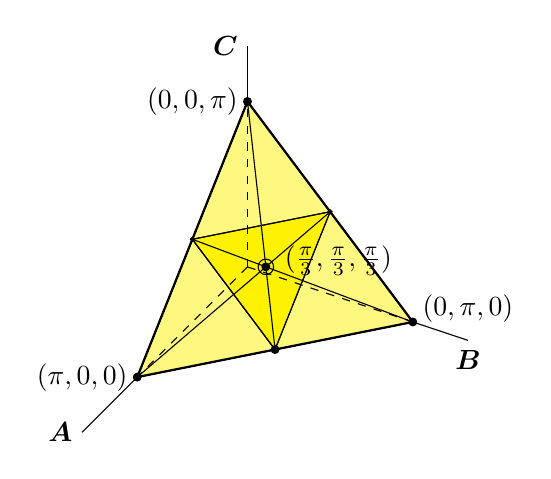
\begin{tikzpicture}[scale=.7]
		%Points
		\filldraw (0,3) circle (2pt); %top
		\filldraw (-2,-2) circle (2pt); %bottom left
		\filldraw (3,-1) circle (2pt); %bottom right
		\filldraw (1/3,0) circle (2pt); %centroid equilateral
		\draw (1/3,0) circle (4pt); %centroid equilateral
		\filldraw (1/2,-3/2) circle (2pt); %bottom midpoint
		\filldraw (-1,1/2) circle (1pt); %left midpoint
		\filldraw (3/2,1) circle (1pt); %right midpoint
		%\filldraw[orange] (-1/4,-1/2) circle (2pt); % right isosceles
		%\draw[orange] (-1/4,-1/2) circle (4pt);
		%Lines
		\draw[thick] (0,3)--(3,-1)--(-2,-2)--(0,3); %perimeter
		\draw (1/2,-3/2)--(-1,1/2)--(3/2,1)--(1/2,-3/2); %triangle of right triangles
		\draw[dashed] (0,0) -- (0,3); %z-axis
		\draw (0,3) -- (0,4); %z-axis end
		\draw[dashed] (0,0) -- (3,-1); %y-axis
		\draw (3,-1) -- (4,-4/3); %y-axis end
		\draw[dashed] (0,0) -- (-2,-2); %x-axis
		\draw (-2,-2) -- (-3,-3); %x-axis end
		\draw (0,3) -- (3,-1); %right side triangle
		\draw (0,3) -- (-2,-2); %left side triangle
		\draw (-2,-2) -- (3,-1); %bottom of triangle
		\draw (-2,-2) -- (3/2,1); %to midpoint on left side.
		\draw (0,3) -- (1/2,-3/2);
		\draw (3,-1) -- (-1,1/2);
		%\draw[ultra thick, red] (1/2,-3/2) -- (-1/4,-1/2);
		%\draw[ultra thick, blue] (-2,-2) -- (1/3,0);
		%\draw[ultra thick, blue] (1/2,-3/2) -- (1/3,0);
		%\draw[ultra thick, dashed, blue] (-2,-2) -- (1/2,-3/2);
		%Nodes
		\fill
		(0,3) node [left] {$(0,0,\pi)$}
		(3,-.75) node [right] {$(0,\pi,0)$}
		(-2,-2) node [left] {$(\pi,0,0)$}
		%(1/2,-1.75) node [below] {$(\tfrac\pi 2,\tfrac\pi 2,0)$}
		%(-1,1/2) node [left] {$(\tfrac\pi 2,0,\tfrac\pi 2)$}
		%(3/2,1) node [right] {$(0,\tfrac\pi 2,\tfrac\pi 2)$}
		(9/18,1/9) node [right] {$(\tfrac{\pi}3,\tfrac{\pi}3,\tfrac{\pi}3)$};
		%(-1/3,-1/2) node [left] {$(\tfrac\pi 2,\tfrac\pi 4,\tfrac\pi 4)$};
		\node[left] at (-3,-3) {$\boldsymbol A$};
		\node[below] at (4,-4/3) {$\boldsymbol B$};
		\node[left] at (0,4) {$\boldsymbol C$};
		%shading
		\begin{scope}[on background layer]
		\draw[fill=yellow!50] (0,3)--(3,-1)--(-2,-2)--(0,3);
		%perimeter of obtuse restricted to x>y>z: (-2,-2) -- (1/2,-3/2) -- (-1/4,-1/2) -- (-2,-2);
		\draw[fill=yellow!100] (1/2,-3/2)--(-1,1/2)--(3/2,1)--(1/2,-3/2);
		%perimeter of acute restricted (1/3,0) -- (1/2,-3/2) -- (-1/4,-1/2) -- (1/3,0);
		\end{scope}
	\end{tikzpicture}
    \caption{Triangle of Triangles $ \T_+$}
    \label{fig:t-of-t}
\end{subfigure}
\hfill
\begin{subfigure}{0.5\textwidth}
    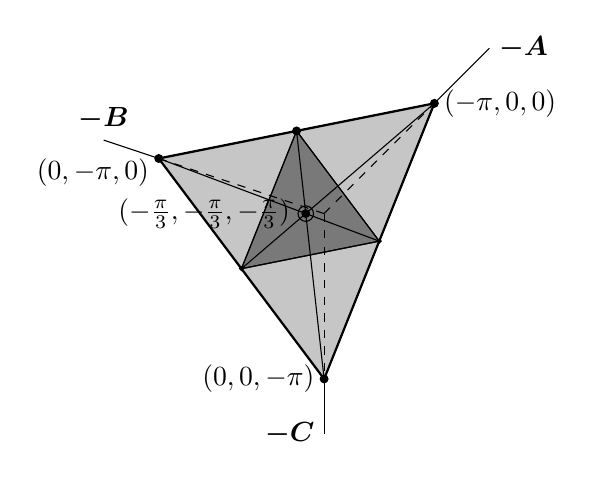
\begin{tikzpicture}[scale=.7]
	    \filldraw (10,-3) circle (2pt); %top
		\filldraw (12,2) circle (2pt); %bottom left
		\filldraw (7,1) circle (2pt); %bottom right
		\filldraw (10-1/3,0) circle (2pt); %centroid equilateral
		\draw (10-1/3,0) circle (4pt); %centroid equilateral
		\filldraw (10-1/2,3/2) circle (2pt); %bottom midpoint
		\filldraw (11,-1/2) circle (1pt); %left midpoint
		\filldraw (10-3/2,-1) circle (1pt); %right midpoint
		%Lines
		\draw[thick] (10,-3)--(7,1)--(12,2)--(10,-3); %perimeter
		\draw (10-1/2,3/2)--(11,-1/2)--(10-3/2,-1)--(10-1/2,3/2); %triangle of right triangles
		\draw[dashed] (10,0) -- (10,-3); %z-axis
		\draw (10,-3) -- (10,-4); %z-axis end
		\draw[dashed] (10,0) -- (7,1); %y-axis
		\draw (7,1) -- (6,4/3); %y-axis end
		\draw[dashed] (10,0) -- (12,2); %x-axis
		\draw (12,2) -- (13,3); %x-axis end
		\draw (10,-3) -- (7,1); %right side triangle
		\draw (10,-3) -- (12,2); %left side triangle
		\draw (12,2) -- (7,1); %bottom of triangle
		\draw (12,2) -- (10-3/2,-1); %to midpoint on left side.
		\draw (10,-3) -- (10-1/2,3/2);
		\draw (7,1) -- (11,-1/2);
		%Nodes
		\fill
		(10,-3) node [left] {$(0,0,-\pi)$}
		(7,.75) node [left] {$(0,-\pi,0)$}
		(12,2) node [right] {$(-\pi,0,0)$}
		(10-4/9,0) node [left] {$(-\tfrac\pi 3,-\tfrac\pi 3,-\tfrac\pi 3)$};
		%(10-1/2,1.75) node [above] {$(-\tfrac\pi 2,-\tfrac\pi 2,0)$}
		%(11,-1/2) node [right] {$(-\tfrac\pi 2,0,-\tfrac\pi 2)$}
		%(10-3/2,-1) node [left] {$(0,-\tfrac\pi 2,-\tfrac\pi 2)$};
		\node[right] at (13,3) {$\boldsymbol{- A}$};
		\node[above] at (6,4/3) {$\boldsymbol {-B}$};
		\node[left] at (10,-4) {$\boldsymbol {-C}$};
		%shading
		\begin{scope}[on background layer]
		\draw[fill=darkgray!30] (10,-3)--(7,1)--(12,2)--(10,-3);
		\draw[fill=darkgray!70] (10-1/2,3/2)--(11,-1/2)--(10-3/2,-1)--(10-1/2,3/2);
		\end{scope}
	\end{tikzpicture}
    \caption{Shadow Triangle of Triangles $\T_-$}
    \label{fig:shadow-t-of-t}
\end{subfigure}
\caption{\hspace{0cm}}
\label{tot+}
\end{figure}



\section{\Large The Torus of Relative Arguments}
\FloatBarrier

In this section we construct another space whose general points represent
similarity classes of nondegenerate labeled, oriented triangles, and 
whose continuity leads to a natural definition of similarity
for degenerate labeled triangles, which form the border regions
$\partial\T_+$ and $\partial\T_-$ above, and with which we will glue $\T_+$ and $\T_-$ together.
The idea is based on the observation that 
a nondegenerate labeled, oriented similarity class $[\tri ABC]$
is completely determined by the two ordered arguments $\xi_A$ and $\xi_B$ relative to
$C$. The triangle can then be 
inscribed in the unit circle, as in Figure~\ref{relarg}, where we write the arguments
with representatives between $0$ and $2\pi$.


\begin{figure}[!h]
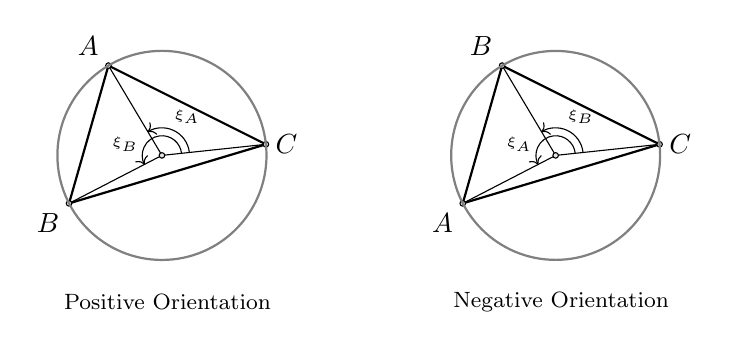
\begin{tikzpicture}
\tkzDefPoints{0/1/A,-.5/-.75/B,2/0/C}
\tkzDrawPolygon[thick](A,B,C)l
\tkzDefTriangleCenter[circum](A,B,C)
\tkzGetPoint{O}
\tkzMarkAngle[size=0.35,->](C,O,A)
%\tkzLabelAngle[pos=0.5,font=\small](C,O,A){$\xi_A$}
\tkzMarkAngle[size=0.25,->](C,O,B)
\tkzDrawSegments[thin](O,A O,B O,C)
\tkzDrawPoints(A,B,C,O)
\tkzLabelPoints[above left](A)
\tkzLabelPoints[right](C)
\tkzLabelPoints[below left](B)
%\tkzLabelPoints(O)
\tkzDefCircle[circum](A,B,C)
\tkzGetPoint{I}
\tkzDrawCircle[thick](I,A)
%%%%%
\tkzDefPoints{4.5/-.75/A, 5/1/B, 7/0/C} %added 5 to x.
\tkzDrawPolygon[thick](B,A,C)
\tkzDefTriangleCenter[circum](B,A,C)
\tkzGetPoint{O}
\tkzMarkAngle[size=0.25,->](C,O,A)
\tkzMarkAngle[size=0.35,->](C,O,B)
%\tkzLabelAngle[pos=0.5,font=\small](C,O,B){$\xi_B$}
\tkzDrawSegments[thin](O,B O,A O,C)
\tkzDrawPoints(B,A,C,O)
\tkzLabelPoints[above left](B)
\tkzLabelPoints[right](C)
\tkzLabelPoints[below left](A)
%\tkzLabelPoints(O)
\tkzDefCircle[circum](A,B,C)
\tkzGetPoint{I}
\tkzDrawCircle[thick](I,A)
%%%%%
\node at (1,.35) {\tiny $\xi_A$};
\node[left] at (.5,0) {\tiny $\xi_B$};
\node[left] at (5.5,0) {\tiny $\xi_A$};
\node at (6,.35) {\tiny $\xi_B$};
\node at (.75,-2) {\footnotesize Positive Orientation};
\node at (5.75,-2) {\footnotesize Negative Orientation};
\end{tikzpicture}
\caption{$\hphantom{}$} %Relative Arguments}
\label{relarg}
\end{figure}

\FloatBarrier

\subsection{Torus of Relative Arguments}
\subsubsection{Construction}
Let $\S^1$ denote the circle Lie group,
$\R^1=(\R^1,+)$ its Lie algebra, and $\exp:\R^1\lr\S^1$
the exponential $\xi\mapsto e^{i\xi}$, which is a homomorphism. 
We call $\xi$ an {\it argument}.
The $\R$-linear homomorphism $\delta_+:\R^3\lr\R^2$ defined by 
$\delta_+(\xi_1,\xi_2,\xi_2)=(\xi_1-\xi_3,\xi_2-\xi_3)$
determines a commutative diagram
{\normalsize
\[\begin{tikzcd}
0\arrow[r]&\R^1\arrow[r,"\Delta"]\arrow[d,"\exp"]&\R^3\arrow[r,"\delta_+"]
\arrow[d,"\exp"]&\R^2\arrow[r]\arrow[d,"\exp"]&0\\
1\arrow[r]&\S^1\arrow[r,"\Delta"]&(\S^1)^3\arrow[r,"\delta"]&\T\arrow[r]&1
\end{tikzcd}\]}

\noindent
where $\Delta$ is the diagonal embedding, and $\T\isom(\S^1)^2$ is a torus.
We call $\R^2$ the {\it plane of relative arguments}.
The maps $\delta_+$ and $\delta$ are split by the $\R$-linear map $\sigma_+:(\xi_1,\xi_2)\mapsto(\xi_1,\xi_2,0)$
and the homomorphism $\sigma:(e^{i\xi_1},e^{i\xi_2})\mapsto(e^{i\xi_1},e^{i\xi_2},1)$, respectively.
Since left multiplication by $\S^1$ is the same as the (left) rotation action by $\SO(2)$, we have
\[\T\;=\;(\S^1)^3/\SO(2)\]
On the other hand, since the kernel of $\exp$ consists of the lattice $\{(2k\pi,2\ell\pi):k,\ell\in\Z\}$,
$\T\;\isom\;\R^2/2\pi\Z^2$, which is the usual definition of the Clifford torus.
\begin{Definition}\label{torus}\rm
\begin{enumerate}[(a)]
\item
The {\it torus of relative arguments} is the abelian torus group $\T$ constructed above,
with points interpreted as ordered triples of points on $\S^1$ up to rotations,
each represented by a unique ordered triple $(e^{i\xi_1},e^{i\xi_2},1)$,
and with pointwise product
$(e^{i\xi_1},e^{i\xi_2},1)\cdot(e^{i\xi_1'},e^{i\xi_2'},1)
=(e^{i(\xi_1+\xi_1')},e^{i(\xi_2+\xi_2')},1)$.
\item
A triple $(e^{i\xi_1},e^{i\xi_2},1)$ is {\it nondegenerate}
if the three points are distinct, and {\it degenerate} otherwise.
Thus a degenerate triple satisfies $\xi_1=2k\pi$, $\xi_2=2k\pi$, or $\xi_1-\xi_2=2k\pi$ for $k\in\Z$.
\item 
A nondegenerate triple has {\it positive orientation} if the forward (left-to-right) reading of 
coordinates in the triple
goes counterclockwise around $\S^1$, and {\it negative orientation} otherwise. 
A degenerate triple has {\it zero orientation}. 
\end{enumerate}
\end{Definition}

\subsection{Connection of $\T$ to Triangles}
Each point $(\xi_1,\xi_2)$ in the plane of relative arguments maps to a point $(e^{i\xi_1},e^{i\xi_2},1)$ 
on $\T$, corresponding to a unique similarity class of labeled, oriented triangle.
We illustrate the plane in Figure~\ref{planerelarg}, with a shaded fundamental
domain $0\leq\xi_1,\xi_2<2\pi$, and solid lines representing the preimage of the degenerate triangles on $\T$.
The fundamental domain is divided into two parts according to the orientations of the corresponding triangles. 

The construction of a borderless parameter space $\T$
arising from Figure~\ref{planerelarg} depends on the incorporation of orientation.
In this space,
a continuous family {\it changes orientation} when it crosses the degenerate border. 
%The plane and the resulting torus thus provide a sensible interpretation 
%of what happens to continuous families that cross the border of degenerate triangles. 
In moduli spaces (such as $\T_+$) that do not take orientation into account, 
a path that intersects the border transversally has a singularity, 
and must reverse course to stay in the space. 
By adding orientation we obtain what we feel is a more natural space.
We will show later that the usual space of (unoriented, unlabeled) similarity classes is a topological quotient.


\begin{figure}[!h]
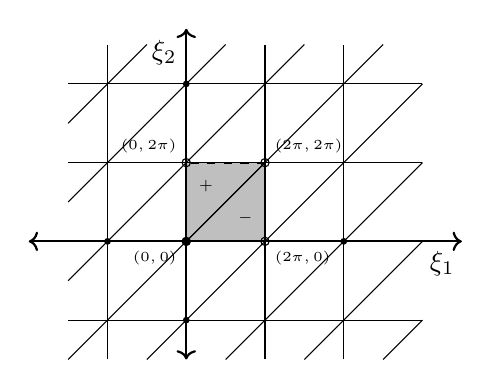
\begin{tikzpicture}
%Points
\filldraw (0,0) circle (1.5pt);
\draw (1,0) circle (1.5pt);
\filldraw (2,0) circle (1pt);
\filldraw (-1,0) circle (1pt);
\draw (0,1) circle (1.5pt);
\filldraw (0,2) circle (1pt);
\filldraw (0,-1) circle (1pt);
\draw (1,1) circle (1.5pt);
\draw[thick,<->] (-2,0)--(3.5,0);
\draw[thick,<->] (0,-1.5)--(0,2.7);
\draw[thick, dashed] (0,0)--(0,1)--(1,1)--(1,0);
\draw (0,0)--(1,1);
\draw (-1,-1.5)--(-1,2.5);
\draw (1,-1.5)--(1,2.5);
\draw (2,-1.5)--(2,2.5);
\draw (-1.5,1)--(3,1);
\draw (-1.5,2)--(3,2);
\draw (-1.5,-1)--(3,-1);
\draw (-1.5,-1.5)--(2.5,2.5);
\draw (-1.5,-.5)--(1.5,2.5);
\draw (-1.5,.5)--(.5,2.5);
\draw (-1.5,1.5)--(-.5,2.5);
\draw (-.5,-1.5)--(3,2);
\draw (.5,-1.5)--(3,1);
\draw (1.5,-1.5)--(3,0);
\draw (2.5,-1.5)--(3,-1);
\node[below] at (3.25,0) {$\xi_1$};
\node[left] at (0,2.4) {$\xi_2$};
\node[below right] at (1,0) {\tiny $(2\pi,0)$};
\node[above left] at (0,1) {\tiny $(0,2\pi)$};
\node[below left] at (0,0) {\tiny $(0,0)$};
\node[above right] at (1,1) {\tiny $(2\pi,2\pi)$};
\node at (.25,.7) {\tiny $+$};
\node at (.75,.3) {\tiny $-$};
%shading
\begin{scope}[on background layer]
\draw[fill=gray!50] (0,0)--(1,0)--(1,1)--(0,1)--(0,0);
\end{scope}
\end{tikzpicture}
\caption{\footnotesize Plane of Relative Arguments}
\label{planerelarg}
\end{figure}

\FloatBarrier
\section{\Large The Torus of Triangles}\label{GlueTofT}
\FloatBarrier

In this section we make the correspondence between points on the torus and labeled
oriented similarity classes more explicit by defining a map $\T_+\sqcup\T_-\lr\T$
from the triangles of triangles of Definition~\ref{LOT} to the torus of Definition~\ref{torus}
giving
us an explicit interior angle description of the triangles represented by points of $\T$, 
and inducing a definition of similarity for degenerate triangles.
This also serves the purpose of imposing on $\T$ the standard uniform
measure implicit in $\T_+\sqcup\T_-$.


\subsection{Map from Triangles of Triangles to Torus of Relative Arguments}
\subsubsection{Construction}\label{map}
A point on $[\tri ABC]=\tri[\alpha,\beta,\gamma]\in\T_+$ satisfies $\alpha,\beta,\gamma\in[0,\pi]$ and $\alpha+\beta+\gamma=\pi$,
and $\tri[\alpha,\beta,\gamma]\in\T_-$ satisfies $\alpha,\beta,\gamma\in[-\pi,0]$ and $\alpha+\beta+\gamma=-\pi$.
Proposition 20 of 
Euclid's Book III (\cite{Euclid}, see also \cite{DJ98}) states,
{\it in a circle the angle at the center is double the angle at 
the circumference when the angles have the same circumference as base.}
\begin{figure}
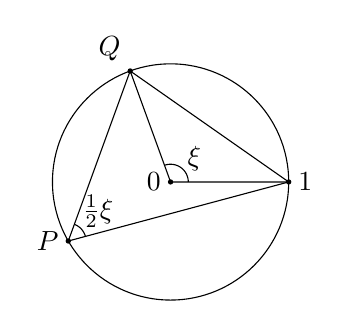
\begin{tikzpicture}[scale=1.5]%Triangle
\draw (0,0) circle (1);
\filldraw (1,0) circle (.5pt);
\filldraw ({cos(110)},{sin(110)}) circle (.5pt);
\filldraw ({cos(210)},{sin(210)}) circle (.5pt);
\filldraw (0,0) circle (.5pt);
\draw (1,0)--({cos(110)},{sin(110)})--({cos(210)},{sin(210)})--(1,0);
\draw (1,0)--(0,0)--({cos(110)},{sin(110)});
%\draw (0,0)--({cos(210)},{sin(210)});
\draw[domain=0:110] plot ({.15*cos(\x)},{.15*sin(\x)});
\draw[domain=15:70] plot ({cos(210)+.15*cos(\x)},{sin(210)+.15*sin(\x)});
\node at (.2,.2) {$\xi$};
\node at ({cos(210)+.25},{sin(210)+.25}) {$\tfrac 12\xi$};
\node[right] at (1,0) {$1$};
\node[left] at (0,0) {$0$};
\node[left] at ({cos(210)},{sin(210)}) {$P$};
\node[above left] at ({cos(110)},{sin(110)}) {$Q$};
\end{tikzpicture}
\caption{\hspace{0cm}}
\label{euclid}
\end{figure}
Therefore if we inscribe the similarity class of 
a nondegenerate triangle $\tri[\alpha,\beta,\gamma]$ in $\S^1$ with third vertex $C=1$, we can compute
the arguments of $A$ and $B$ from $\alpha$ and $\beta$, and so define
a map from the triangles of triangles to the torus of relative arguments. 
To wit, if the triangle is positively oriented then $\alpha,\beta,\gamma>0$,
and then $P=B$, $Q=A$, and
$\beta=\frac 12\xi>0$ in Figure~\ref{euclid}.
Since $\xi$ is the counterclockwise argument of $A$, $A=e^{i2\beta}$, and similarly $B=e^{i(2\pi-2\alpha)}=e^{-i2\alpha}$.
The resulting triple $(e^{i2\beta},e^{-i2\alpha},1)$ is positively oriented, since the left-to-right reading
goes counterclockwise around the circle.
If the triangle is negatively oriented then 
$\alpha,\beta,\gamma<0$, and $P=A$, $Q=B$, and $\alpha=-\frac 12\xi<0$. Then $B=e^{-i2\alpha}$, and similarly
$A=e^{-i(2\pi-2\beta)}=e^{i2\beta}$. This time the resulting triple $(e^{i2\beta},e^{-i2\alpha},1)$ is negatively oriented. 
This motivates the following definition.

\begin{Definition}\label{rho}\rm
Suppose $\tri=\tri[\alpha,\beta,\gamma]\in\T_+\sqcup\T_-$, with $\alpha,\beta,\gamma\in[0,\pi]$
if $\tri\in\T_+$, and $\alpha,\beta,\gamma\in[-\pi,0]$ if $\tri\in\T_-$.
Define
\begin{align*}
\rho\,:\,\T_+\sqcup\T_-&\lr\,\T\\
\tri[\alpha,\beta,\gamma]&\longmapsto
(e^{i2\beta},e^{-i2\alpha},1)
\end{align*}
\end{Definition}

\begin{Theorem}\label{main theorem}
The map $\rho$ is surjective, preserves orientation, 
and inscribes $\tri[\alpha,\beta,\gamma]\in\T_+\sqcup\T_-$
in $\S^1$ as the triple $(e^{i2\beta},e^{-i2\alpha},1)$.
%In particular $\rho$ maps the degenerate triangles onto the degenerate triples of $\T$.

Let $\partial(\partial(\T_+\sqcup\T_-))$
denote the six vertices of the border $\partial(\T_+\sqcup\T_-)$, and let
%$(\partial(\T_+\sqcup\T_-))^\circ=
$(\partial\T_+)^\circ\sqcup(\partial\T_-)^\circ$ 
denote the interior of the border.
Assume $0\leq\alpha,\beta\leq\pi$.
Then the degenerate points of $\T$ have preimages
\begin{align*}
\rho^{-1}(1,1,1)&=\{\tri[\pm\pi,0,0],\tri[0,\pm\pi,0],\tri[0,0,\pm\pi]\}=\partial(\partial(\T_+\sqcup\T_-))\\
\rho^{-1}(e^{i2\beta},1,1)&=\{\tri[0,\beta,\pi-\beta]\in(\partial\T_+)^\circ,\;\tri[0,-\pi+\beta,-\beta]
\in(\partial\T_-)^\circ\}\\
\rho^{-1}(1,e^{-i2\alpha},1)&=\{\tri[\alpha,0,\pi-\alpha]
\in(\partial\T_+)^\circ,\;\tri[-\pi+\alpha,0,-\alpha]\in(\partial\T_-)^\circ\}\\
\rho^{-1}(e^{i2\beta},e^{i2\beta},1)&=\{\tri[\pi-\beta,\beta,0]
\in(\partial\T_+)^\circ,\;\tri[-\beta,-\pi+\beta,0]\in(\partial\T_-)^\circ\}
\end{align*}
Thus the preimage of $(1,1,1)\in\T$ consists of the six vertex points
of $\T_+\sqcup\T_-$, 
and the preimage of every other
degenerate point of $\T$ has two preimage points, one on $(\partial\T_+)^\circ$ and one on $(\partial\T_-)^\circ$.
\end{Theorem}

\begin{proof}
By Construction~\eqref{map}, $\rho$ inscribes every nondegenerate
oriented triangle $\tri[\alpha,\beta,\gamma]$ in $\S^1$ as a triple of points $(P,Q,1)$ with the same orientation.
Conversely, every such triple is obviously in the image of such a triangle.
Therefore $\rho$ is surjective and preserves orientation on nondegenerate points of $\T$.
We will show surjectivity at the
degenerate triples below by explicitly computing their preimages.

Suppose $\tri=\tri[\alpha,\beta,\gamma]$ is degenerate, i.e., has orientation zero. 
To show $\rho(\tri)$ is degenerate is to show that two of the points $\{e^{i2\beta},e^{-i2\alpha},1\}$
are the same.
Since $\tri$ is degenerate, by Definition~\ref{triangles} one of its interior angles
$\alpha,\beta$ or $\gamma$ is $0$.
If it's $\alpha$ or $\beta$ we are done, because then $e^{-i2\alpha}=1$ or $e^{i2\beta}=1$.
If it's neither then $\gamma=0$, $\alpha+\beta=\pm\pi$, and $e^{i2\beta}=e^{-i2\alpha}$,
and again we are done.

%Suppose $\tri\in\T_+^\circ$, so $\alpha,\beta\in(0,\pi)$. Since $\alpha+\beta<\pi$ we have
%$0<2\beta<2\pi-2\alpha<2\pi$, so the forward reading of $(e^{i2\beta}, e^{-i2\alpha},1)$ 
%goes counterclockwise around $\S^1$.
%Therefore $\rho(\tri)$ is positively oriented by definition.
%Suppose $\tri\in\T_-^\circ$, then $-\pi<\alpha+\beta<0$,
%hence $-2\pi<-2\pi-2\alpha<2\beta<0$, 
%so the forward reading of $(e^{i2\beta}, e^{-i2\alpha},1)$ goes clockwise around $\S^1$,
%hence $\rho(\tri)$ is negatively oriented.

Now we check the preimages. If $\rho(\tri[\alpha,\beta,\gamma])=(1,1,1)$ then
$2\beta=2k\pi$ for some $k$, hence $\beta$ is a multiple of $\pi$, and similarly for $\alpha$;
since the sum of all three is $\pi$, the same goes for $\gamma$.
Therefore $\tri[\alpha,\beta,\gamma]$ must be one of the six vertexes,
and all, of course, map to $(1,1,1)$.
The remaining degenerate triples contain exactly two distinct points: $(P,1,1),(1,Q,1)$, or $(P,P,1)$.
Putting $P=e^{i2\beta}$ and $Q=e^{-i2\alpha}$ shows
$\rho$ maps the stated preimages onto the corresponding degenerate triples.
Since every degenerate triangle is accounted for in some preimage, this completes the proof.
\end{proof}

\begin{Definition}\rm
Degenerate triangles 
in $\partial\T_+\sqcup\partial\T_-$ are {\it similar} if either each has two zero interior
angles, or they share one zero interior
angle, and the other two angles are anti-transpositions of each other. Thus
the distinct similarity classes are of form
\begin{gather*}
\tri[\pi,0,0]=\tri[-\pi,0,0]=\tri[0,\pm\pi,0]=\tri[0,0,\pm\pi]\\
\tri[0,\beta,\gamma]=\tri[0,-\gamma,-\beta]\qquad\tri[\alpha,0,\gamma]=\tri[-\gamma,0,-\alpha]
\qquad \tri[\alpha,\beta,0]=\tri[-\beta,-\alpha,0]
\end{gather*}
\end{Definition}

Using these identifications we immediately obtain
the following.

\begin{Corollary}
The set of similarity classes of labeled, oriented, possibily degenerate
triangles is parameterized by the abelian torus group
\[\frac{\T_+\sqcup\T_-}{\partial\T_+\sim\partial\T_-}\,\approx\,\T\] 
where the gluing of border points is determined by $\rho$
as in Theorem~\ref{main theorem} and Figure~\ref{gluedcor}, identifying all
six vertex points with the identity $(1,1,1)\in\T$, and
pairs of (degenerate) border points as
\[
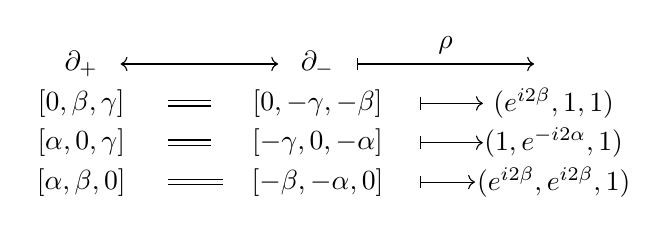
\begin{tikzpicture}
\draw[<->] (-1.5,0)--(.5,0);
\draw[|->] (1.5,0)--(3.75,0);
\draw[double equal sign distance] (-.9,-.5)--(-.35,-.5);
\draw[double equal sign distance] (-.9,-1)--(-.35,-1);
\draw[double equal sign distance] (-.9,-1.5)--(-.2,-1.5);
\draw[|->] (2.3,-.5)--(3.1,-.5);
\draw[|->] (2.3,-1)--(3.1,-1);
\draw[|->] (2.3,-1.5)--(3,-1.5);
\node[above] at (2.625,0) {$\rho$};
\node at (-2,0) {$\partial\T_+$};
\node at (1,0) {$\partial\T_-$};
\node at (4,0) {$\T$};
\node at (-2,-.5) {$\tri[0,\beta,\gamma]$};
\node at (1,-.5) {$\tri[0,-\gamma,-\beta]$};
\node at (4,-.5) {$(e^{i2\beta},1,1)$};
\node at (-2,-1) {$\tri[\alpha,0,\gamma]$};
\node at (1,-1) {$\tri[-\gamma,0,-\alpha]$};
\node at (4,-1) {$(1,e^{-i2\alpha},1)$};
\node at (-2,-1.5) {$\tri[\alpha,\beta,0]$};
\node at (1,-1.5) {$\tri[-\beta,-\alpha,0]$};
\node at (4,-1.5) {$(e^{i2\beta},e^{i2\beta},1)$};
\end{tikzpicture}
\]
\end{Corollary}

\begin{figure}
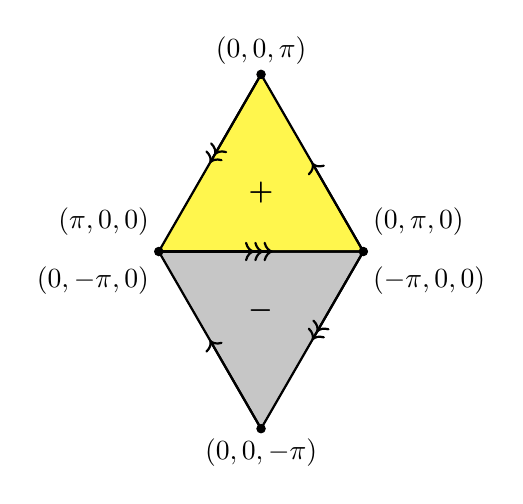
\begin{tikzpicture}[scale=3]
\filldraw (0,-1/4) circle (.5pt); %bottom
\filldraw ({-sqrt(3)/4},1/2) circle (.5pt); %left
\filldraw ({+sqrt(3)/4},1/2) circle (.5pt); %right
\filldraw (0,5/4) circle (.5pt); %top
%Lines on right side
\draw[thick] (0,-1/4)--({+sqrt(3)/4},1/2)--({-sqrt(3)/4},1/2)--(0,-1/4); %bottom
\draw[thick] (0,5/4) --({+sqrt(3)/4},1/2)--({-sqrt(3)/4},1/2)--(0,5/4); %top
\draw[thick, ->] (0,-1/4)--({-sqrt(3)/8},1/8); %bottom
\draw[thick, ->>] ({+sqrt(3)/4},1/2)--({+sqrt(3)/8},1/8); %bottom
\draw[thick, ->>>] ({-sqrt(3)/4},1/2)--(0.05,1/2); %middle
\draw[thick, ->] ({+sqrt(3)/4},1/2)--({+sqrt(3)/8},7/8);
\draw[thick, ->>] (0,5/4)--({-sqrt(3)/8},7/8); %bottom
%shading on right side
\begin{scope}[on background layer]
\draw[fill=darkgray!30] (0,-1/4)--({+sqrt(3)/4},1/2)--({-sqrt(3)/4},1/2)--(0,-1/4);
\draw[fill=yellow!70] (0,5/4) --({+sqrt(3)/4},1/2)--({-sqrt(3)/4},1/2)--(0,5/4);
\end{scope}
%nodes on right side
\node[below] at (0,-1/4) {$(0,0,-\pi)$};
\node[left] at ({-sqrt(3)/4},1/2+1/8) {$(\pi,0,0)$};
\node[right] at ({+sqrt(3)/4},1/2+1/8) {$(0,\pi,0)$};
\node at ({-.15-sqrt(3)/4},1/2) {\tiny $\Vvert$};
\node at ({.15+sqrt(3)/4},1/2) {\tiny $\Vvert$};
\node[left] at ({-sqrt(3)/4},1/2-1/8) {$(0,-\pi,0)$};
\node[right] at ({+sqrt(3)/4},1/2-1/8) {$(-\pi,0,0)$};
\node[above] at (0,5/4) {$(0,0,\pi)$};
\node at (0,1/4) {$\boldsymbol -$};
\node at (0,3/4) {$\boldsymbol +$};
%%%%%%%%%%%%%%%%%%%%%%%%%%%%%%%%%%%%%%%%%%%%%%%%%%%%%%%%%%%%%%%%%%%%%%%%%%%%%%%%%%%%%%%%%%
%%%%%%%%%%%%%%%%%%%%%%%%%%%%%%%%%%%%%%%%%%%%%%%%%%%%%%%%%%%%%%%%%%%%%%%%%%%%%%%%%%%%%%%%%%
\end{tikzpicture}
\caption{\hspace{0cm}}
\label{gluedcor}
\end{figure}


\FloatBarrier
\subsection{Image in $\T$ of Labeled, Oriented Triangle Types}
An element of $\T$ is given by a triple in $\S^1$ whose third entry is $1$.
In this subsection we describe the basic types as they appear in $\S^1$.
\begin{enumerate}[\rm(a)]
\item
By Definition~\ref{triangles} a degenerate triangle has at least one zero interior angle,
so the image of its similarity class under $\rho$ is $(e^{i\xi},1,1)$,
$(1,e^{i\xi},1)$, or $(e^{i\xi},e^{i\xi},1)$, inscribed in $\S^1$ as a chord.
Specifically, on similarity classes we have:
\begin{enumerate}[$\circ$]
\item
The degenerate equilateral triangle has image the identity triple $(1,1,1)$.
\item
The three degenerate isosceles triangles that are not equilateral have images
the diameter $(-1,1,1)$, $(1,-1,1)$, or $(-1,-1,1)$.
\item
The (infinitely many)
degenerate scalene triangles have images $(e^{i\xi},1,1)$, $(1,e^{i\xi},1)$, or $(e^{i\xi},e^{i\xi},1)$,
with $e^{i\xi}\neq \pm 1$.
\end{enumerate}
\[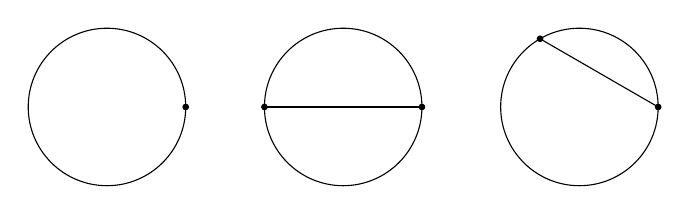
\begin{tikzpicture}
\filldraw (-2,0) circle (1pt);
\filldraw (1,0) circle (1pt);
\filldraw (-1,0) circle (1pt);
\filldraw (4,0) circle (1pt);
\filldraw (2.5,{sqrt(3)/2}) circle (1pt);
\draw (-3,0) circle (1cm);
\draw (0,0) circle (1cm);
\draw (3,0) circle (1cm);
\draw (-1,0)--(1,0);
\draw (4,0)--(2.5,{sqrt(3)/2});
\end{tikzpicture}\]
\item
Nondegenerate triangles have positive or negative orientation, and all angles
of absolute value between $0$ and $\pi$.
Specifically, on $\T_+^\circ\sqcup\T_-^\circ$ we have:
\begin{enumerate}[$\bullet$]
\item
The two nondegenerate equilateral triangles 
have images $(e^{i2\pi/3},e^{i4\pi/3},1)$ and $(e^{i4\pi/3},e^{i2\pi/3},1)$.
\item
The (infinitely many) nondegenerate isosceles triangles have 
%form $\tri[\alpha,\alpha,\gamma]$, $\tri[\alpha,\beta,\alpha]$, or $\tri[\alpha,\gamma,\gamma]$.
images $(e^{i\xi},e^{-i\xi},1)$, $(e^{i2\xi},e^{i\xi},1)$, or $(e^{i\xi},e^{i2\xi},1)$,
depending on whether the vertex is at $C$, $B$, or $A$.
\item
The (infinitely many) nondegenerate right triangles have 
%form $\tri[\alpha,\beta,\gamma]$, with $\alpha,\beta$, or $\gamma$ equal to $\pm\frac\pi 2$. Its 
images $(e^{i\xi},-1,1)$, $(-1,e^{i\xi},1)$, or $(e^{i\xi},-e^{i\xi},1)$, depending on whether 
the right angle is at $A$, $B$, or $C$.
\item
The (infinitely many) nondegenerate scalene triangles have
%form $\tri[\alpha,\beta,\gamma]$ with $\alpha,\beta,\gamma$ all distinct. 
images $(e^{i\xi_1},e^{i\xi_2},1)$ not of any of the previous types.
\end{enumerate}
\end{enumerate}


\section{\Large Distinguished Subgroups}
\FloatBarrier

\subsection{Subgroup Structure of Distinguished Triangle Classes}
The group structure of $\T$ is compatible with triangle types, in the sense that the latter form
basic algebraic structures: elements of finite order, subgroups, and cosets.

\begin{Theorem}
The standard triangle types form the following distinguished subgroups and cosets of the torus of triangles $\T$.
\begin{enumerate}[\rm(a)]
\item
The three equilateral triangle classes form a group of order $3$, with the two nondegenerate classes as generators and
the degenerate class as the identity.
\item
The three degenerate nonequilateral isosceles classes each generate a group of order $2$, with the degenerate
equilateral class as the identity.
\item
The six nondegenerate right isosceles classes generate three cyclic groups of order $4$, 
each containing a degenerate nonequilateral isosceles class (of order $2$).
\item
The three types of isosceles triangle classes $\{{\sf I}_A,{\sf I}_B,{\sf I}_C\}$, 
distinguished by vertex, form three circle subgroups.
\item
The three types of degenerate classes $\{{\sf D}_A,{\sf D}_B,{\sf D}_C\}$, 
distinguished by vertex, form three circle subgroups.
\item
The three types of right triangle classes $\{{\sf R}_A,{\sf R}_B,{\sf R}_C\}$, distinguished by vertex, 
are cosets of the degenerate subgroups ${\sf D}_i$, and their images are the unique
elements of order two in the quotients $\T/{\sf D}_i$.
\end{enumerate}
\end{Theorem}

\begin{proof}
For (d),(e), and (f) it will suffice to write down the stated subgroups; checking they form subgroups is trivial.
In the following we refer to the lie algebra of relative arguments, whose fundamental domain, 
divided into positive and negative orientations, is Figure~\ref{fund}.
\begin{figure}[h]
%\centering
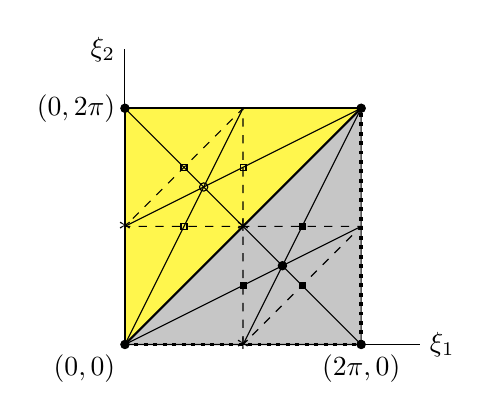
\begin{tikzpicture}
[scale=1.5]
%Points
\filldraw (0,0) circle (1pt); %mid bottom
\filldraw (0,2) circle (1pt); %top left
\filldraw (2,2) circle (1pt); %top right
\filldraw (2,0) circle (1pt); %botom right
\draw (2/3,4/3) circle (1pt); %equilateral positive
\filldraw (4/3,2/3) circle (1pt); %equilateral negative
%\draw (1,1) circle (1.5pt); %degen isosceles
%\draw (1,0) circle (1.5pt); %degen isosceles
%\draw (0,1) circle (1.5pt); %degen isosceles
\draw (.475,.975) rectangle (.525,1.025);
\draw (.5-.025,1.5-.025) rectangle (.5+.025,1.5+.025);
\draw (1-.025,1.5-.025) rectangle (1+.025,1.5+.025);
\filldraw (1-.025,.5-.025) rectangle (1+.025,.5+.025);
\filldraw (1.5-.025,.5-.025) rectangle (1.5+.025,.5+.025);
\filldraw (1.5-.025,1-.025) rectangle (1.5+.025,1+.025);
%\filldraw (1,1) circle (.5pt); %isosceles point in Q_C
%\filldraw (1,2) circle (.5pt); %isosceles point in Q_C
%\filldraw (0,1) circle (.5pt); %isosceles point in Q_C
%Lines
\draw[line width=0.5mm, dotted] (0,0)--(2,0)--(2,2); %perimeter bottom
\draw[thick] (0,0)--(0,2)--(2,2); %perimeter
\draw[thick] (0,0)--(2,2); %diagonal
\draw (0,0)--(0,2.5); %y-axis.
\draw (0,0)--(2.5,0); %x-axis.
\draw[thin] (0,2)--(2,0); %thin isosceles line
\draw[thin] (0,1)--(2,2); %thin isosceles line
\draw[thin] (0,0)--(1,2); %thin isosceles line
\draw[thin] (0,0)--(2,1);
\draw[thin] (1,0)--(2,2);
%Colors
\begin{scope}[on background layer]
\draw[fill=darkgray!30] (0,0)--(2,2)--(2,0)--(0,0); %lower right
\draw[fill=yellow!70] (0,0)--(2,2)--(0,2)--(0,0); %yellow perimeter
\draw[dashed, fill=yellow!70] (1,1)--(1,2)--(0,1)--(1,1); %yellow acute
\draw[dashed, fill=darkgray!30] (1,0)--(1,1)--(2,1)--(1,0); %lower right acute
\end{scope}
%Nodes
\node[left] at (0,2) {$(0,2\pi)$};
\node[below] at (2,0) {$(2\pi,0)$};
\node[below left] at (0,0) {$(0,0)$};
\node[right] at (2.5,0) {$\xi_1$};
\node[left] at (0,2.5) {$\xi_2$};
\node at (1,1) {$*$};
\node at (0,1) {$*$};
\node at (1,0) {$*$};
\end{tikzpicture}
\caption{\hspace{0cm}} 
\label{fund}
\end{figure}
\begin{enumerate}[$\bullet$]
\item
In the plane of relative arguments,
the additive groups ${\sf d}_A=\{(\xi,0)\}$, ${\sf d_B}=\{(0,\xi)\}$, and ${\sf d_C}=\{(\xi,\xi)\}$
define three subgroups of degenerate triangles in $\T\equiv\sigma(\T)\subset\S^1$:
\[{\sf D}_A=\{(e^{i\xi},1,1)\}\qquad
{\sf D}_B=\{(1,e^{i\xi},1)\}\qquad {\sf D}_C=\{(e^{i\xi},e^{i\xi},1)\}\]
\item
The three cosets ${\sf r}_A=(0,\pi)+{\sf d}_A$, ${\sf r}_B=(\pi,0)+{\sf d}_B$, and ${\sf r}_C=(0,\pi)+{\sf d}_C$
correspond to the right triangles:
\[{\sf R}_A=(1,-1,1)\cdot{\sf D}_A=\{(e^{i\xi},-1,1)\}\quad 
{\sf R}_B=(-1,1,1)\cdot{\sf D}_B=\{(-1,e^{i\xi},1)\}\quad
{\sf R}_C=(1,-1,1)\cdot{\sf D}_C=\{(e^{i\xi},-e^{i\xi},1)\}\]
The degenerate right triples comprise the set $\{(1,-1,1),(-1,1,1),(-1,-1,1)\}$.
\item
The subgroups 
${\sf i}_A=\{(\xi,2\xi)\}$,
${\sf i}_B=\{(2\xi,\xi)\}$, and
${\sf i}_C=\{(\xi,-\xi)\}$,
correspond to the isosceles triangles in $\T$:
\[
{\sf I}_A=\{(e^{i\xi},e^{i2\xi},1)\}\qquad{\sf I}_B=\{(e^{i2\xi},e^{i\xi},1)\}\qquad
{\sf I}_C=\{(e^{i\xi},e^{-i\xi},1)\}
\]
\end{enumerate}
(a): The two nondegenerate equilateral classes $\pm(e^{i2\pi/3},e^{i4\pi/3},1)$ are in 
the intersection ${\sf I}_A\cap{\sf I}_B\cap{\sf I}_C$ of the isosceles subgroups,
marked as the centroids of the yellow and gray triangles of Figure~\ref{fund}.
They are mutually inverse, forming together with the degenerate equilateral class $(1,1,1)$ 
a subgroup of order $3$.

\noindent
(b): The three degenerate nonequilateral isosceles classes 
form the set \[\{(e^{i\pi},1,1),(1,e^{i\pi},1),(e^{i\pi},e^{i\pi},1)\}\]
marked by $*$'s in Figure~\ref{fund}.
Each is the unique order-two element of the subgroups ${\sf D}_A,{\sf D}_B,{\sf D}_C$,
respectively.

\noindent
(c): The six nondegenerate right isosceles classes form the set
\[\{\pm(e^{i\pi/2},e^{i\pi},1),\pm(e^{i\pi/2},e^{i3\pi/2},1),\pm(e^{i\pi},e^{i3\pi/2},1)\}\]
marked with square points in Figure~\ref{fund}. Each has order $4$ and square equal
to one of the three degenerate nonequilateral isosceles classes.
\end{proof}



\begin{Remark}
The symmetry of the plane of relative arguments suggests
some other families not included in the standard taxonomies:
\begin{enumerate}[$\bullet$]
\item
The perpendicular ``anti-isosceles'' subgroups 
${\sf i}_A^\perp=\{(-2\xi,\xi)\}$,
${\sf i}_B^\perp=\{(\xi,-2\xi)\}$, and
${\sf i}_C^\perp={\sf d}_C=\{(\xi,\xi)\}$ 
define subgroups
\[
{\sf I}_A^\perp=\{(e^{-i2\xi},e^{i\xi},1)\}\qquad
{\sf I}_B^\perp=\{(e^{i\xi},e^{-i2\xi},1)\}\qquad
{\sf I}_C^\perp={\sf D}_C=\{(e^{i\xi},e^{i\xi},1)\}
\]
\item
The distinguished coset $(0,\pi)+{\sf i}_C=\{(\xi,\pi-\xi)\}$ defines the coset
of ``anti-right'' triangles.
\[(1,-1,1)\cdot{\sf I}_C=\{(e^{i\xi},-e^{-i\xi},1)\}\]
\end{enumerate}
When graphed in Figure~\ref{fund},
%or on the triangles of triangles $\T_+\sqcup\T_-/\sim$, 
the above objects make
a complete graph with nine vertices.
\end{Remark}

\FloatBarrier
\section{\Large Absolute Similarity Classes}

Let
\[\pm S_3:=S_3\times\br{\pm e}=\{\pm e,\pm(123),\pm(132),\pm(23),\pm(13),\pm(12)\}\] a group of order $12$
isomorphic to the dihedral group $D_6=\br{r,s}$, where in our notation
$r\equiv-(123)$ is counterclockwise rotation of a regular hexagon by $\pi/3$, $r^3\equiv-e$, and $s\equiv-(12)$
is reflection about the horizontal axis:
\[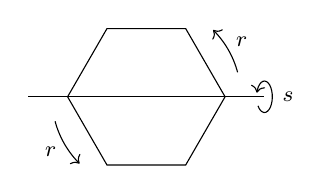
\begin{tikzpicture}
\draw[thin] (-1.5,0)--(1.5,0);
\draw (1,0)--({cos(60)},{sin(60)})--({cos(120)},{sin(120)})
--(-1,0)--({cos(240)},{sin(240)})--({cos(300)},{sin(300)})--(1,0); %hexagon
\draw[domain=15:45, ->] plot ({1.2*cos(\x)},{1.2*sin(\x)});
\draw[domain=195:225, ->] plot ({1.2*cos(\x)},{1.2*sin(\x)});
\draw[domain=-145:165, ->] plot ({1.5+.1*cos(\x)},{.2*sin(\x)});
\node at ({1.4*cos(30)},{1.4*sin(30)}) {\footnotesize $r$};
\node at ({1.4*cos(210)},{1.4*sin(210)}) {\footnotesize $r$};
\node at (1.8,0) {\footnotesize $s$};
\end{tikzpicture}\]
The permutation representation \[\pm S_3\lr\GL_3(\R)\] defines an action on $\R^3$ that stabilizes $\Delta$.
Explicitly,
\begin{align*}\pm S_3\times\R^3&\lr\R^3\\
(\pm\sigma,(\theta_1,\theta_2,\theta_3))&\longmapsto(\pm\theta_{\sigma(1)},\pm\theta_{\sigma(2)},\pm\theta_{\sigma(3)})
\end{align*}
Since both $\delta$ and the splitting map $\sigma$ are $\R$-linear, the induced representation
$\pm S_3\lr\GL_2$ acts on the plane of relative arguments $\R^2$. 
Explicitly,
$\pm\sigma(\theta_1-\theta_3,\theta_2-\theta_3)
=\pm(\theta_{\sigma(1)}-\theta_{\sigma(3)},\theta_{\sigma(2)}-\theta_{\sigma(3)})$.
The image of the corresponding two-dimensional permutation representation is
\begin{gather*}
\pm e=\pm\sdbmx{1&0\\0&1}\qquad\pm(123)=\pm\sdbmx{-1&1\\-1&0}\qquad\pm(132)=\pm\sdbmx{0&-1\\1&-1}\\
\pm(12)=\pm\sdbmx{0&1\\1&0}\qquad\pm(13)=\pm\sdbmx{-1&0\\-1&1}\qquad\pm(23)=\pm\sdbmx{1&-1\\0&-1}
\end{gather*}

Since these actions do not change the (unordered) absolute values of the arguments in a triple,
they stabilize the kernel of $\exp$, and induce actions on $(\S^1)^3$ and $\T$.
%Note the actions on $\R^3$ do not change the (unordered) absolute values of the angles in a triple.
On $\S^1$ negation acts as complex conjugation, which 
reverses the orientation of a nondegenerate triple since it turns an ordering that
goes counterclockwise to one that goes clockwise.

The induced action on interior angles in $\sfrac{\T_+\sqcup\T_-}{\sim}$
is represented by Figure~\ref{hex}, in which the triangles of triangles are inscribed
in a regular hexagon.
\begin{figure}
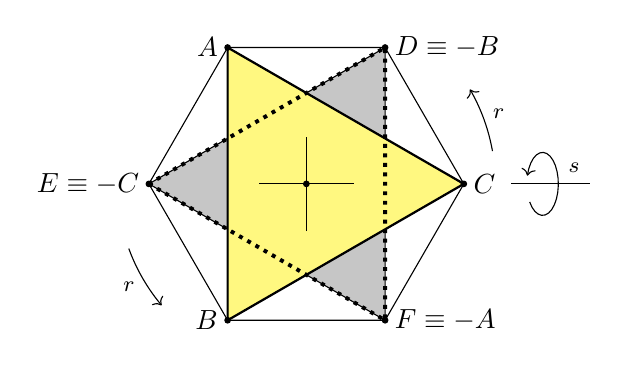
\begin{tikzpicture}[scale=2]%Hexagon 
\filldraw (1,0) circle (.5pt);
\filldraw (0,0) circle (.5pt);
\filldraw ({cos(60)},{sin(60)}) circle (.5pt);
\filldraw ({cos(120)},{sin(120)}) circle (.5pt);
\filldraw ({cos(180)},{sin(180)}) circle (.5pt);
\filldraw ({cos(240)},{sin(240)}) circle (.5pt);
\filldraw ({cos(300)},{sin(300)}) circle (.5pt);
\draw[thick] (1,0)--({cos(120)},{sin(120)})--({cos(240)},{sin(240)})--(1,0); %gold
\draw[line width=0.5mm, dotted] (-1,0)--({cos(300)},{sin(300)})--({cos(60)},{sin(60)})--(-1,0); %shadow
\draw[thin] (1,0)--({cos(60)},{sin(60)})--({cos(120)},{sin(120)})
--(-1,0)--({cos(240)},{sin(240)})--({cos(300)},{sin(300)})--(1,0); %hexagon
\draw (-.3,0)--(.3,0);
\draw (0,-.3)--(0,.3);
\draw (1.3,0)--(1.8,0);
%\draw (-1.3,0)--(-1.8,0);
%arcs
\draw[domain=-145:165, ->] plot ({1.5+.1*cos(\x)},{.2*sin(\x)});
\draw[domain=10:30, ->] plot ({1.2*cos(\x)},{1.2*sin(\x)});
\draw[domain=200:220, ->] plot ({1.2*cos(\x)},{1.2*sin(\x)});
%nodes
\node[left] at (-1,0) {$E\equiv-C$};
\node[right] at (1,0) {$C$};
\node[right] at ({cos(60)},{sin(60)}) {$D\equiv-B$};
\node[right] at ({cos(300)},{sin(300)}) {$F\equiv-A$};
\node[left] at ({cos(120)},{sin(120)}) {$A$};
\node[left] at ({cos(240)},{sin(240)}) {$B$};
\node at (1.7,.1) {\footnotesize $s$};
\node at ({1.3*cos(20)},{1.3*sin(20)}) {\footnotesize $r$};
\node at ({1.3*cos(210)},{1.3*sin(210)}) {\footnotesize $r$};
%shading
\begin{scope}[on background layer]
\draw[fill=darkgray!30] (-1,0)--({cos(300)},{sin(300)})--({cos(60)},{sin(60)})--(-1,0);
\draw[fill=yellow!50] (1,0)--({cos(120)},{sin(120)})--({cos(240)},{sin(240)})--(1,0);
\end{scope}
\end{tikzpicture}
\caption{\hspace{0cm}}
\label{hex}
\end{figure}
The $A,B,C$-axes and $-A,-B,-C$-axes are the same as those in Figure~\ref{tot+},
and the gluing is $AB\leftrightarrow DF, BC\leftrightarrow ED, AC\leftrightarrow EF$.
The $2\times 2$ matrix action on relative arguments shows the induced action is given by the map
\[
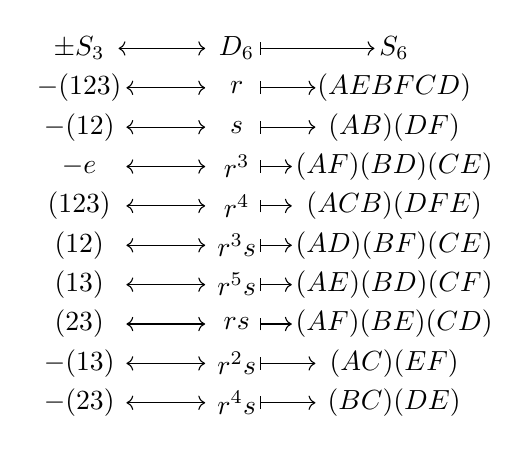
\begin{tikzpicture}
\draw[<->] (-1.5,0)--(-.4,0);
\draw[|->] (.3,0)--(1.75,0);
\draw[<->] (-1.4,-.5)--(-.4,-.5);
\draw[<->] (-1.4,-1)--(-.4,-1);
\draw[<->] (-1.4,-1.5)--(-.4,-1.5);
\draw[<->] (-1.4,-2)--(-.4,-2);
\draw[<->] (-1.4,-2.5)--(-.4,-2.5);
\draw[<->] (-1.4,-3)--(-.4,-3);
\draw[<->] (-1.4,-3.5)--(-.4,-3.5);
\draw[<->] (-1.4,-4)--(-.4,-4);
\draw[<->] (-1.4,-4.5)--(-.4,-4.5);
\draw[|->] (.3,-.5)--(1,-.5);
\draw[|->] (.3,-1)--(1,-1);
\draw[|->] (.3,-1.5)--(.7,-1.5);
\draw[|->] (.3,-2)--(.7,-2);
\draw[|->] (.3,-2.5)--(.7,-2.5);
\draw[|->] (.3,-3)--(.7,-3);
\draw[|->] (.3,-3.5)--(.7,-3.5);
\draw[|->] (.3,-4)--(1,-4);
\draw[|->] (.3,-4.5)--(1,-4.5);
\node at (-2,0) {$\pm S_3$};
\node at (-2,-.5) {$-(123)$};
\node at (-2,-1) {$-(12)$};
\node at (-2,-1.5) {$-e$};
\node at (-2,-2) {$(123)$};
\node at (-2,-2.5) {$(12)$};
\node at (-2,-3) {$(13)$};
\node at (-2,-3.5) {$(23)$};
\node at (-2,-4) {$-(13)$};
\node at (-2,-4.5) {$-(23)$};
\node at (0,0) {$D_6$};
\node at (0,-.5) {$r$};
\node at (0,-1) {$s$};
\node at (0,-1.5) {$r^3$};
\node at (0,-2) {$r^4$};
\node at (0,-2.5) {$r^3 s$};
\node at (0,-3) {$r^5 s$};
\node at (0,-3.5) {$rs$};
\node at (0,-4) {$r^2 s$};
\node at (0,-4.5) {$r^4 s$};
\node at (2,0) {$S_6$};
\node at (2,-.5) {$(AEBFCD)$};
\node at (2,-1) {$(AB)(DF)$};
\node at (2,-1.5) {$(AF)(BD)(CE)$};
\node at (2,-2) {$(ACB)(DFE)$};
\node at (2,-2.5) {$(AD)(BF)(CE)$};
\node at (2,-3) {$(AE)(BD)(CF)$};
\node at (2,-3.5) {$(AF)(BE)(CD)$};
\node at (2,-4) {$(AC)(EF)$};
\node at (2,-4.5) {$(BC)(DE)$};
\end{tikzpicture}
\]

The elements that preserve orientation form the subgroup \[D_3\isom\big\langle r^2,s\big\rangle\leq\pm S_3\]
which then acts separately on $\T_+$ and $\T_-$.

\begin{Theorem}\label{orbitspace}
The orbit space $[\T]$ of $\T$ under $\pm S_3\isom D_6$ is the set of similarity classes of triangles.
\end{Theorem}

\begin{proof}
Let
$\tri_1=\tri[\theta_1,\theta_2,\theta_3]$ and $\tri_2=\tri[\psi_1,\psi_2,\psi_3]$. 
Write $\tri_1\isom\tri_2$ for similar, and $[\tri_1]=[\tri_2]$ for same orbit. Then
\begin{align*}
\tri_1\isom\tri_2\,&\Leftrightarrow\,\pm\{\theta_1,\theta_2,\theta_3\}=\{\psi_1,\psi_2,\psi_3\}
\,\Leftrightarrow\;\exists\sigma\,:\;(\psi_1,\psi_2,\psi_3)=\pm(\theta_{\sigma(1)},\theta_{\sigma(2)},\theta_{\sigma(3)})\\
&\,\Leftrightarrow\,[\tri_1]=[\tri_2]
\end{align*}
\end{proof}

\subsection{Triangle Multiplicities}
The differences in symmetry
distinguish the scalene, right, isosceles, and equilateral degenerate and nondegenerate triangles,
and this is measured by the sizes of their stabilizer subgroups.

\begin{Definition}\rm
The {\it multiplicity} $\mult(\tri)$ of $\tri\in\T$ is the order of
$\stab(\tri)\leq\pm S_3\isom D_6$. 
\end{Definition}

\begin{Theorem}\label{mult}
The multiplicities of similarity classes of labeled, oriented, possibly degenerate
triangles are as follows.
\begin{enumerate}[\rm(a)]
\item
The degenerate equilateral triangle has multiplicity $12$.
\item
The two nondegenerate equilateral triangles have multiplicity $6$.
\item
The three degenerate nonequilateral isosceles triangles have multiplicity $4$.
\item
Degenerate scalene triangles each have multiplicity $2$.
\item
Nondegenerate nonequilateral isosceles triangles each have multiplicity $2$.
\item
Nondegenerate scalene triangles each have multiplicity $1$.
\end{enumerate}
\end{Theorem}

\begin{proof}
We refer to Figure~\ref{hex} and compute using $D_6$.

The degenerate equilateral $\tri_e$ is represented by any of the vertices in
Figure~\ref{hex}, hence its orbit has lenght $1$, and it is fixed by $D_6$.
Therefore $\mult(\tri_e)=12$.

The nondegenerate equilateral triangles $\tri_{E_+}$ and $\tri_{E_-}$ are conjugate by the element $r^3 s$,
and each has stabilizer $\langle r^2,s\rangle\isom D_3$, hence $\mult(\tri_{E_+})=\mult(\tri_{E_-})=6$.

The degenerate nonequilateral isosceles triangles 
$\left\{\tri[0,\tfrac\pi 2,\tfrac\pi 2],\tri[\tfrac\pi 2,0,\tfrac\pi 2],\tri[\tfrac\pi 2,\tfrac\pi 2,0]\right\}$
are conjugate by rotations. We compute $\stab(\tri[\tfrac\pi 2,\tfrac\pi 2,0])=\br{r^3,s}\isom C_2\times C_2$,
hence $\mult(\tri[\tfrac\pi 2,\tfrac\pi 2,0])=4$, and the others follow suit.

Degenerate scalene triangles have orbits of length 6 under the elements
of $\br{r}$. The stabilizer of
$\tri=\tri[\alpha,\beta,0]$ (with $\alpha,\beta\neq 0,\pm\tfrac\pi 2,\pm\pi$)
is $\stab(\tri)=\langle r^3 s\rangle$, hence $\mult(\tri)=2$.  

Nondegenerate nonequilateral isosceles triangles have orbits of length 6 under $\br{r}$.
If $\tri\in{\sf I}_C$ then $\stab(\tri)=\br{s}$,
hence $\mult(\tri)=2$.

Nondegenerate scalene triangles $\tri$ have orbits of length 12,
and stabilizers $\stab\left(\tri(\alpha,\beta,\gamma)\right)=\br{e}$, where 
$\alpha,\beta,\gamma$ are distinct. Therefore $\mult(\tri)=1$.
\end{proof}

\FloatBarrier

\section{\Large Measure}

\FloatBarrier

\begin{figure}
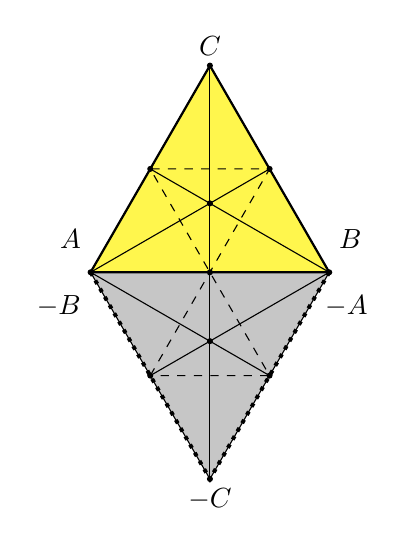
\begin{tikzpicture}[scale=1.75]
\filldraw (0,-1/2) circle (.5pt); %bottom
\filldraw ({-sqrt(3)/2},1) circle (.5pt); %left
\filldraw ({+sqrt(3)/2},1) circle (.5pt); %right
\filldraw (0,5/2) circle (.5pt); %top
\filldraw ({sqrt(3)/4},7/4) circle (.5pt);
\filldraw ({-sqrt(3)/4},7/4) circle (.5pt);
\filldraw ({sqrt(3)/4},1/4) circle (.5pt);
\filldraw ({-sqrt(3)/4},1/4) circle (.5pt);
\filldraw (0,1) circle (.5pt);
\filldraw (0,1/2) circle (.5pt); %center gray
\filldraw (0,3/2) circle (.5pt); %center yellow
%Lines on right side
\draw[line width=0.5mm, dotted] ({-sqrt(3)/2},1)--(0,-1/2)--({+sqrt(3)/2},1);%bottom
\draw[thick] (0,5/2) --({+sqrt(3)/2},1)--({-sqrt(3)/2},1)--(0,5/2); %top perimeter
\draw[dashed] ({-sqrt(3)/4},1/4)--({sqrt(3)/4},7/4)--({-sqrt(3)/4},7/4)--({sqrt(3)/4},1/4)--({-sqrt(3)/4},1/4);
\draw ({-sqrt(3)/2},1)--({+sqrt(3)/4},7/4); %i_1
\draw ({-sqrt(3)/4},1/4)--({sqrt(3)/2},1); %i_1
\draw ({+sqrt(3)/2},1)--({-sqrt(3)/4},7/4); %i_2
\draw ({sqrt(3)/4},1/4)--({-sqrt(3)/2},1); %i_2
\draw (0,5/2)--(0,-1/2); %i_3
%\draw[thick, ->] (0,-1/2)--({-sqrt(3)/4},1/4);  %bottom
%\draw[thick, ->>] ({+sqrt(3)/2},1)--({+sqrt(3)/4},1/4); %bottom
%\draw[thick, ->>>] ({-sqrt(3)/2},1)--(.2,1); %middle
%\draw[thick, ->] ({sqrt(3)/2},1)--({+sqrt(3)/4},7/4);
%\draw[thick, ->>] (0,5/2)--({-sqrt(3)/4},7/4); %bottom
%shading on right side
\begin{scope}[on background layer]
\draw[fill=darkgray!30] (0,-1/2)--({+sqrt(3)/2},1)--({-sqrt(3)/2},1)--(0,-1/2);
\draw[fill=yellow!70] (0,5/2) --({+sqrt(3)/2},1)--({-sqrt(3)/2},1)--(0,5/2);
\end{scope}
%nodes on right side
\node[below] at (0,-1/2) {$-C$};
\node[above left] at ({-sqrt(3)/2},1+.1) {$A$};
\node[above right] at ({+sqrt(3)/2},1.1) {$B$};
\node[left] at ({-sqrt(3)/2},1) {\tiny $\Vvert$};
\node[right] at ({sqrt(3)/2},1) {\tiny $\Vvert$};
\node[below left] at ({-sqrt(3)/2},1-.1) {$-B$};
\node[below right] at ({+sqrt(3)/2-.1},1-.1) {$-A$};
\node[above] at (0,5/2) {$C$};
%%%%%%%%%%%%%%%%%%%%%%%%%%%%%%%%%%%%%%%%%%%%%%%%%%%%%%%%%%%%%%%%%%%%%%%%%%%%%%%%%%%%%%%%%%
%%%%%%%%%%%%%%%%%%%%%%%%%%%%%%%%%%%%%%%%%%%%%%%%%%%%%%%%%%%%%%%%%%%%%%%%%%%%%%%%%%%%%%%%%%
\end{tikzpicture}
\caption{\hspace{0cm}}
\label{glued}
\end{figure}




By Theorem~\ref{orbitspace} the similarity classes of triangles are repeated in $\T$ according to their
multiplicity under the action of $D_6$. This motivates the following definition.

\begin{Definition}\label{measure}\rm
Let ${\sf F}\subset\T$ be a family of similarity classes of labeled, oriented triangles, and let $[{\sf F}]$ denote the
corresponding set of similarity classes in the orbit space $[\T]\equiv\T/D_6$.
The {\it relative measure} of $[{\sf F}]$ is
\[\mu([{\sf F}])=\mult(\tri)\cdot|{\sf F}|\]
where $|{\sf F}|$
is the Euclidean measure in $\T$ under the metric of $\T$ defined by 
$\rho:\T_+\sqcup\T_-\lr\T$ in Definition~\ref{rho}, and $\tri\in{\sf F}$ is a generic element.
\end{Definition}

The relative measure of a two-parameter family is given by its Euclidean measure, since all generic points of
such families have multiplicity one.

\begin{Theorem}
Let $\sf O,A,I,R,D,OI,AI$ be the families of similarity classes of labeled, oriented
triangles in $\T$ that are
obtuse, acute, isosceles, right, degenerate, obtuse isosceles, and 
acute isosceles, respectively.
Then the relative measures are
\begin{enumerate}[\rm(a)]
\item
$\mu(\T)=\sqrt 3\pi^2$; $\mu({\sf O})=\frac{3\sqrt 3}4\pi^2$; $\mu({\sf A})=\frac{\sqrt 3}4\pi^2$;
\item
$\mu({\sf I})=6\sqrt 6\pi$; $\mu({\sf R})=3\sqrt 2\pi$; $\mu({\sf D})=6\sqrt 2\pi$; and
$\mu({\sf OI})=\mu({\sf AI})=3\sqrt 6\pi$.
\end{enumerate}
In particular we have the following ratios:
\[[{\sf O}:{\sf A}]=[3:1]\qquad [{\sf I}:{\sf AI}]=[{\sf I}:{\sf OI}]=[2:1]\qquad
[{\sf I}:{\sf R}]=[2\sqrt 3:1]\qquad [{\sf D}:{\sf R}]=[2:1]
\]
\end{Theorem}

\begin{proof}
Using Figure~\ref{glued} we easily compute
$|{\sf T}|=\sqrt 3\pi^2$, $|{\sf O}|=\frac{3\sqrt 3}4\pi^2$, and $|{\sf A}|=\frac{\sqrt 3}4\pi^2$.
Generic elements of these two-parameter families all have multiplicity one, so these
are the relative measures as defined in Definition~\ref{measure}.

For the one-parameter families we compute
$|{\sf I}|=3\sqrt 6\pi$, $|{\sf R}|=3\sqrt 2\pi$, $|{\sf D}|=3\sqrt 2\pi$, $|{\sf OI}|=\frac{3\sqrt 6}2\pi$,
and $|{\sf AI}|=\frac{3\sqrt 6}2\pi$.
Generic degenerate elements, which are scalene, and generic nondegenerate isosceles both
have multiplicity two, and a generic right triangle has multiplicity one, by Theorem~\ref{mult}.
Therefore the relative measures are as stated in these cases.
For obtuse and acute isosceles triangles the multiplicites are $2$, so they have the same
relative measure $3\sqrt 6\pi$.
The ratios follow immediately.
\end{proof}


\bibliographystyle{alpha} %other choices are plain or abbrv or alpha
\bibliography{../../mathdocs.bib}

\end{document}



%Picture of triangle with arguments, more general.
\begin{figure}
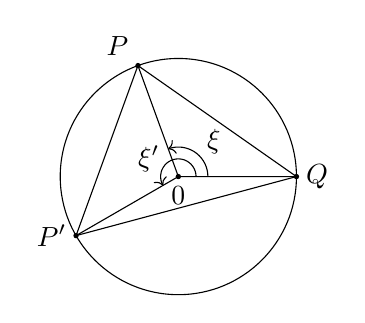
\begin{tikzpicture}[scale=1.5]%Triangle with arguments
\draw (0,0) circle (1);
\filldraw (1,0) circle (.5pt);
\filldraw ({cos(110)},{sin(110)}) circle (.5pt);
\filldraw ({cos(210)},{sin(210)}) circle (.5pt);
\filldraw (0,0) circle (.5pt);
\draw (1,0)--({cos(110)},{sin(110)})--({cos(210)},{sin(210)})--(1,0);
\draw (1,0)--(0,0)--({cos(110)},{sin(110)});
\draw (0,0)--({cos(210)},{sin(210)});
\draw[domain=0:110,->] plot ({.25*cos(\x)},{.25*sin(\x)});
\draw[domain=0:210,->] plot ({.15*cos(\x)},{.15*sin(\x)});
\node at (.3,.3) {$\xi$};
\node at (-.25,.15) {$\xi'$};
\node[right] at (1,0) {$Q$};
\node[below] at (0,0) {$0$};
\node[left] at ({cos(210)},{sin(210)}) {$P'$};
\node[above left] at ({cos(110)},{sin(110)}) {$P$};
\end{tikzpicture}
\caption{\hspace{0cm}}
\label{relarg}
\end{figure}



%\begin{figure}[h]
%	\centering
%	\includegraphics[width=0.4\textwidth]{pics/torus-simple-two-loops.png}
%	\caption{The Torus of Triangles with a Trivial and Nontrivial Loop. The trivial loop is light purple, and the nontrivial loop is dark purple.}
%	\label{fig:torus-simple}
%\end{figure}

\begin{figure}[h]
	\centering
	\begin{subfigure}{0.45\textwidth}
	\centering
	\definecolorseries{first}{rgb}{last}{red}{yellow}
\definecolorseries{second}{rgb}{last}{yellow}{blue}
\definecolorseries{third}{rgb}{last}{blue}{red}
\begin{tikzpicture}[scale=.75]
	    \def\outRadius{2} % outcircle
	    \def\penRadius{0.75*pi*(1-sqrt(2)/2)} % circle in \xi_A,\xi_B plane
	    \def\xA{pi*(sqrt(2)/2)}
	    \def\yA{pi*(2-(sqrt(2)/2))}
	    \tkzDefPoint(0,0){O}
	    \tkzDefPoint(0:\outRadius){C}
	    
	    \resetcolorseries[15]{first}
	    \foreach \t in {0,0.05,...,0.65}{
	    	\tkzDefPoint(\outRadius*cos(\penRadius*cos(\t*pi)+\xA),\outRadius*sin(\penRadius*cos(\t*pi)+\xA)){A}
	    	\tkzDefPoint(\outRadius*cos(\penRadius*sin(\t*pi)+\yA),\outRadius*sin(\penRadius*sin(\t*pi)+\yA)){B}
	     \draw [color=first!!+](A) -- (B) -- (C) -- (A);
		}
		\resetcolorseries[15]{second}
        \foreach \t in {0.65,0.7,...,1.35}{
	    	\tkzDefPoint(\outRadius*cos(\penRadius*cos(\t*pi)+\xA),\outRadius*sin(\penRadius*cos(\t*pi)+\xA)){A}
	    	\tkzDefPoint(\outRadius*cos(\penRadius*sin(\t*pi)+\yA),\outRadius*sin(\penRadius*sin(\t*pi)+\yA)){B}
	     \draw [color=second!!+](A) -- (B) -- (C) -- (A);
		}
		\resetcolorseries[15]{third}
        \foreach \t in {1.35,1.4,...,2}{
	    	\tkzDefPoint(\outRadius*cos(\penRadius*cos(\t*pi)+\xA),\outRadius*sin(\penRadius*cos(\t*pi)+\xA)){A}
	    	\tkzDefPoint(\outRadius*cos(\penRadius*sin(\t*pi)+\yA),\outRadius*sin(\penRadius*sin(\t*pi)+\yA)){B}
	     \draw [color=third!!+](A) -- (B) -- (C) -- (A);
		}
		% special triangle
		\def\arg{0.75} %make sure to change for other figure as well
		\tkzDefPoint(\outRadius*cos(\penRadius*cos(\arg*pi)+\xA),\outRadius*sin(\penRadius*cos(\arg*pi)+\xA)){A}
	    \tkzDefPoint(\outRadius*cos(\penRadius*sin(\arg*pi)+\yA),\outRadius*sin(\penRadius*sin(\arg*pi)+\yA)){B}
	    \draw [thick,black](A) -- (B) -- (C) -- (A);
	    \tkzDrawCircle[thick, black](O,C)
	    \tkzDrawPoints[black](A,B,C)
	    \tkzLabelPoint[above](A){$A$}
	    \tkzLabelPoint[below](B){$B$}
	    \tkzLabelPoint[right](C){$C$}
\end{tikzpicture}
\caption{A Trivial Loop of Triangles.}
\label{fig:trivial-intro}	
	\end{subfigure}
	%\hfill
	\begin{subfigure}{0.5\textwidth}
	\centering
\definecolorseries{first}{rgb}{last}{red}{yellow}
\definecolorseries{second}{rgb}{last}{yellow}{blue}
\definecolorseries{third}{rgb}{last}{blue}{red}
\begin{tikzpicture}[scale=.75]
	    \def\outRadius{2} % outcircle
	    \tkzDefPoint(0,0){O}
	    \tkzDefPoint(0:\outRadius){C}
	    \tkzDefPoint(120: \outRadius){A}
	    \resetcolorseries[13]{first}
	    \foreach \t in {0,10,...,120}{
	    	\tkzDefPoint(\t:\outRadius){B}
	     \draw [color=first!!+](A) -- (B) -- (C) -- (A);
		}
 		\resetcolorseries[13]{second}
        \foreach \t in {120,130,...,240}{
	    	\tkzDefPoint(\t:\outRadius){B}
	     \draw [color=second!!+](A) -- (B) -- (C) -- (A);
		}
 		\resetcolorseries[13]{third}
        \foreach \t in {250,260,...,350}{
	    	\tkzDefPoint(\t:\outRadius){B}
	     \draw [color=third!!+](A) -- (B) -- (C) -- (A);
		}
		% special triangle
		\def\arg{240} %make sure to change for other figure as well
	    \tkzDefPoint(\arg:\outRadius){B}
	    \draw [thick,black](A) -- (B) -- (C) -- (A);
	    \tkzDrawCircle[thick, black](O,C)
	    \tkzDrawPoints[black](A,B,C)
	    \tkzLabelPoint[above](A){$A$}
	    \tkzLabelPoint[below](B){$B$}
	    \tkzLabelPoint[right](C){$C$}
\end{tikzpicture}
\caption{A Nontrivial Loop of Triangles.}
\label{fig:nontrivial-intro}
	\end{subfigure}
	\caption{The evolution is from blue triangles to red to orange to yellow. $C$ is fixed; both $A$ and $B$
	vary on the left, but only $B$ varies on the right.}%Trivial and Nontrivial Loops of Triangles}
	\label{fig:family-intro}
\end{figure}
 
%See  MSC Primary number 51M04




\




{\color{purple}
\section{Triangles of Triangles}




Though we call $\T_+$ a moduli space, it is not one in a strict sense, because some
of the points have nontrivial multiplicities. Specifically,
the triangles $\T_+$ and $\T_-$ have symmetries corresponding to the
six angle orderings: three reflections about
the three altitudes, and three rotations (including the identity). Each symmetry fixes the center
point, which is the equilateral similarity class, and each reflection fixes an altitude, which
comprise the isosceles classes. We acknowledge this by assigning
multiplicities: $1$ to the scalene points, $2$ to the isosceles points, and $6$ to the equilateral point.
When counted with its multiplicity, every unordered oriented similarity class appears 
a total of six times. 

\subsection{Using $\T_+$ to Compute Things}\label{ComputeThings}
We like the representation of the space of triangles in Figure~\ref{fig:shadow-t-of-t}(a),
because it seems natural and is easy to analyze geometrically.
%\begin{figure}
%\centering
%\begin{tikzpicture}[scale=2]
%%Points
%\filldraw ({sqrt(3)/2},-1/2) circle (1pt); %bottom right
%\filldraw ({-sqrt(3)/2},-1/2) circle (1pt); %bottom left
%\filldraw (0,1) circle (1pt); %top
%\filldraw (0,0) circle (1pt); %centroid equilateral
%\draw (0,0) circle (2pt); %centroid
%\filldraw (0,-1/2) circle (.5pt); %bottom midpoint
%\filldraw ({-sqrt(3)/4},1/4) circle (.5pt);
%\filldraw ({sqrt(3)/4},1/4) circle (.5pt);
%%\filldraw[orange] (0,1/4) circle (.5pt); %right isosceles
%%\filldraw[orange] ({sqrt(3)/8},-1/8) circle (.5pt); %right isosceles
%%\filldraw[orange] ({-sqrt(3)/8},-1/8) circle (.5pt); %right isosceles
%%Lines
%\draw (0,1)--({-sqrt(3)/2},-1/2)--({sqrt(3)/2},-1/2)--(0,1); %outside triangle
%\draw (0,-1/2)--({sqrt(3)/4},1/4)--({-sqrt(3)/4},1/4)--(0,-1/2); %inside triangle
%\draw ({-sqrt(3)/2},-1/2)--({sqrt(3)/4},1/4);
%\draw ({sqrt(3)/2},-1/2)--({-sqrt(3)/4},1/4);
%\draw (0,1)--(0,-1/2);
%%shading
%\begin{scope}[on background layer]
%\draw[fill=yellow!100] (0,-1/2)--({sqrt(3)/4},1/4)--({-sqrt(3)/4},1/4)--(0,-1/2);
%\draw[fill=yellow!30] (0,1)--({-sqrt(3)/4},1/4)--({sqrt(3)/4},1/4)--(0,1); 
%\draw[fill=yellow!30] ({-sqrt(3)/4},1/4)--({-sqrt(3)/2},-1/2)--(0,-1/2)--({-sqrt(3)/4},1/4); 
%\draw[fill=yellow!30] ({sqrt(3)/4},1/4)--({sqrt(3)/2},-1/2)--(0,-1/2)--({sqrt(3)/4},1/4); 
%\end{scope}
%%nodes
%\node[below left] at ({-sqrt(3)/2},-1/2) {$(\pi,0,0)$};
%\node[below right] at ({sqrt(3)/2},-1/2) {$(0,\pi,0)$};
%\node[above left] at (0,1) {$(0,0,\pi)$};
%\end{tikzpicture}
%\caption{The Triangle of Triangles}
%\label{fig:t-of-t-simple}
%\end{figure}
It is not original, see e.g. \cite[Figure 2]{ES15}.
With it we can compute things like dimension and relative measure.
It shows, for example, that the acute and obtuse loci are two-dimensional,
reflecting the fact that a triangle in either category is uniquely determined
by two of its angles.
It also shows the loci of isosceles and right triangles is one-dimensional,
reflecting the fact that one number suffices to specify a triangle in those categories.
Additionally, the triangle of triangles predicts
\begin{enumerate}
\item
The ratio of obtuse to isosceles is $[3:1]$. This is because the triangle of acute triangles
is the inscribed triangle, one of four equilateral triangles that partition the triangle of triangles.
\item
The ratio of obtuse-isosceles to acute-isosceles is $[1:1]$. This is because the altitudes 
represent isosceles triangles, and exactly half of each altitude lies in the triangle acute triangles.
\item
The ratio of isosceles to right triangle is $2\cdot\left[\tfrac{\sqrt 3}2:\tfrac 12\right]=2\sqrt 3$:
The ratio of the three altitudes, which describe the isosceles triangles, 
to the perimeter of the inscribed triangle, which represents the right triangles,
is $\sin(\pi/3)/\cos(\pi/3)=\sqrt 3$, and we obtain $2\sqrt 3$ since the isosceles points 
appear with multiplicity two.
\end{enumerate}
Though this parameter space is ``natural'', there are other natural-seeming candidates, 
and, as mentioned above, they sometimes give different predictions for these numbers.
The reason, discussed in depth in \cite{Port}, is essentially that each one implicitly contains
a definition for the term ``random triangle'', and different constructions can differ
in their definitions, yielding different ratios.

\section{\bf The Torus of Triangles}

Although we have just defined a triangle of triangles, we intend to replace it with something
more general. As mentioned in the introduction,
this paper was motivated by the question of what should happen if a continuous family
of triangles should ``breach the border''.
We have our answer in the following: 

\begin{Theorem}
The set of labeled oriented similarity classes of triangles is naturally parameterized by a topological torus.
In particular, $\partial\T_+$ and $\partial(\T_-)$ naturally glue together to make
a space $\sf{TT}=\T_+\sqcup(\T_-)/\sim$ representing the similarity classes of labeled, oriented,
possibly degenerate triangles.
\end{Theorem}

\begin{proof}
For any three points $A,B,C$ inscribed in a circle,
let $\xi_A=\arg(A)-\arg(C)$, $\xi_B=\arg(B)-\arg(C)$, the ``relative arguments'' of the points $A,B,C$, where an argument
is traversed counterclockwise from a fixed ray (see Figure \ref{fig:relatives}).
\begin{figure}[!h]
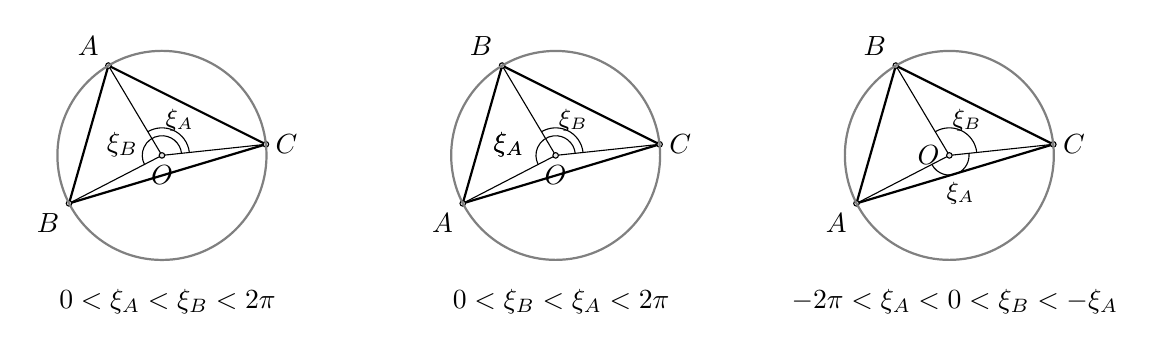
\begin{tikzpicture}
\tkzDefPoints{0/1/A,-.5/-.75/B,2/0/C}
\tkzDrawPolygon[thick](A,B,C)l
\tkzDefTriangleCenter[circum](A,B,C)
\tkzGetPoint{O}
\tkzMarkAngle[size=0.35](C,O,A)
\tkzLabelAngle[pos=0.5,font=\small](C,O,A){$\xi_A$}
\tkzMarkAngle[size=0.25](C,O,B)
\tkzDrawSegments[thin](O,A O,B O,C)
\tkzDrawPoints(A,B,C,O)
\tkzLabelPoints[above left](A)
\tkzLabelPoints[right](C)
\tkzLabelPoints[below left](B)
\tkzLabelPoints(O)
\tkzDefCircle[circum](A,B,C)
\tkzGetPoint{I}
\tkzDrawCircle[thick](I,A)
\node[left] at (.5,0) {$\xi_B$};
%%%%%
\tkzDefPoints{4.5/-.75/A, 5/1/B, 7/0/C} %added 5 to x.
\tkzDrawPolygon[thick](B,A,C)
\tkzDefTriangleCenter[circum](B,A,C)
\tkzGetPoint{O}
\tkzMarkAngle[size=0.25](C,O,A)
\tkzMarkAngle[size=0.35](C,O,B)
\tkzLabelAngle[pos=0.5,font=\small](C,O,B){$\xi_B$}
\tkzDrawSegments[thin](O,B O,A O,C)
\tkzDrawPoints(B,A,C,O)
\tkzLabelPoints[above left](B)
\tkzLabelPoints[right](C)
\tkzLabelPoints[below left](A)
\tkzLabelPoints(O)
\tkzDefCircle[circum](A,B,C)
\tkzGetPoint{I}
\tkzDrawCircle[thick](I,A)
\node[left] at (5.4,0) {$\xi_A$};
%%%%%
\tkzDefPoints{9.5/-.75/A, 10/1/B, 12/0/C} %added 10 to x.
\tkzDrawPolygon[thick](B,A,C)
\tkzDefTriangleCenter[circum](B,A,C)
\tkzGetPoint{O}
\tkzMarkAngle[size=0.25](A,O,C)
\tkzLabelAngle[pos=0.5,font=\small](A,O,C){$\xi_A$}
\tkzMarkAngle[size=0.35](C,O,B)
\tkzLabelAngle[pos=0.5,font=\small](C,O,B){$\xi_B$}
\tkzDrawSegments[thin](O,B O,A O,C)
\tkzDrawPoints(B,A,C,O)
\tkzLabelPoints[above left](B)
\tkzLabelPoints[right](C)
\tkzLabelPoints[below left](A)
\tkzLabelPoints[left](O)
\tkzDefCircle[circum](A,B,C)
\tkzGetPoint{I}
\tkzDrawCircle[thick](I,A)
\node[left] at (5.4,0) {$\xi_A$};
\node at (.75,-2) {$0<\xi_A < \xi_B<2\pi$};
\node at (5.75,-2) {$0<\xi_B<\xi_A<2\pi$};
\node at (10.75,-2) {$-2\pi<\xi_A<0<\xi_B<-\xi_A$};
\end{tikzpicture}
\caption{Samples of Relative Arguments}
\label{fig:relatives}
\end{figure}


Let $\sf R$ be the $\xi_A \xi_B$-plane, shown 
in Figure \ref{fig:region-r}.
\begin{figure}
\centering
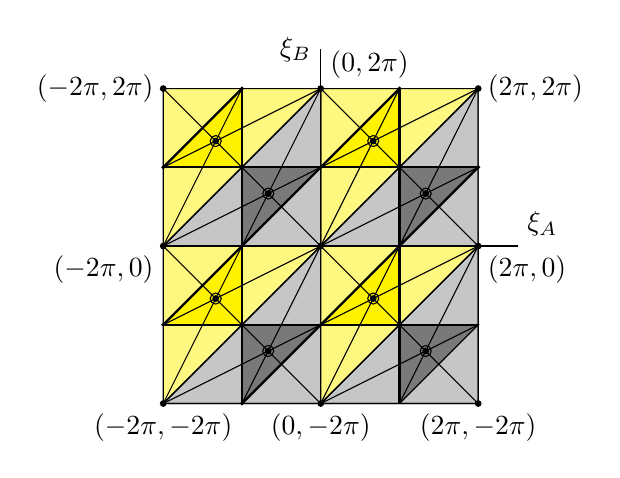
\begin{tikzpicture}%[scale=1.25]
%Points
\filldraw (0,0) circle (1pt);
\filldraw (0,2) circle (1pt); %mid left
\filldraw (2,2) circle (1pt); %mid right
\filldraw (2,0) circle (1pt); %lower right
\filldraw (-2,0) circle (1pt); %lower left
\filldraw (2,4) circle (1pt); %upper right
\filldraw (1,1) circle (.5pt); %isosceles point in Q_C
\filldraw (1,2) circle (.5pt); %isosceles point in Q_C
\filldraw (0,1) circle (.5pt); %isosceles point in Q_C
\filldraw (2,3) circle (.5pt);%isosceles in Q_B
\filldraw (1,3) circle (.5pt); %isosceles in Q_B
\filldraw (-1,0) circle (.5pt); %isosceles in Q_A
\filldraw (-1,1) circle (.5pt); %isosceles in Q_A
\filldraw (0,4) circle (.5pt); %top point on \xi_B axis.
\filldraw (2/3,4/3) circle (1pt); %equilateral in T
\draw (2/3,4/3) circle (2pt); %equilateral in T
\filldraw (4/3,2/3) circle (1pt); %equilateral in Q_C
\draw (4/3,2/3) circle (2pt); %equilateral in Q_C
\filldraw (4/3,2/3+2) circle (1pt); %equilateral in Q_A
\draw (4/3,2/3+2) circle (2pt); %equilateral in Q_A
\filldraw (4/3-2,2/3) circle (1pt); %equilateral in Q_B
\draw (4/3-2,2/3) circle (2pt); %equilateral in Q_B
% adding upper left part
\filldraw (-2,2) circle (1pt);
\filldraw (-2,4) circle (1pt);
\filldraw (0,4) circle (1pt);
\filldraw (-2,1) circle (.5pt);
\filldraw (-2,3) circle (.5pt);
\filldraw (-1,2) circle (.5pt);
\filldraw (-1,3) circle (.5pt);
\filldraw (-1,4) circle (.5pt);
\filldraw (0,3) circle (.5pt);
\filldraw (0,4) circle (.5pt);
\filldraw (1,4) circle (.5pt);
\filldraw (-1-1/3,4/3) circle (1pt); %equilateral in lower left yellow
\draw (-1-1/3,4/3) circle (2pt); %equilateral in lower left yellow
\filldraw (-1-1/3,3+1/3) circle (1pt); %equilateral in upper left yellow
\draw (-1-1/3,3+1/3) circle (2pt); %equilateral in upper left yellow
\filldraw (2/3,1/3+3) circle (1pt); %equilateral in upper right yellow
\draw (2/3,1/3+3) circle (2pt); %equilateral in upper right yellow
\filldraw (-2/3,2+2/3) circle (1pt); %equilateral in upper left gray
\draw (-2/3,2+2/3) circle (2pt); %equilateral in upper left gray

%Lines
\draw (0,2)--(0,4.5); %y-axis.
\draw (0,2)--(2.5,2); %x-axis.
\draw[] (0,0)--(0,2)--(2,2)--(2,0)--(0,0); %perimeter of OG pic
\draw[] (0,0)--(2,2); %diagonal of OG pic
\draw[] (-2,2)--(0,4); %diagonal of upper left pic
\draw[] (-2,0)--(2,4)--(2,0)--(-2,0); %perimater of T#
\draw[] (-2,0)--(-2,4)--(2,4); %perimeter of upper half
\draw[] (-2,2)--(0,2)--(0,4); %perimeter of upper left square
%\draw (0,1)--(1,1)--(1,2)--(0,1); %dark yellow triangle
%\draw (1,0)--(1,1)--(2,1)--(1,0); %black triangle
\draw[thick,black] (-2,1)--(2,1); %horizontal
\draw[thick,black] (-1,0)--(-1,4); %vertical
\draw[thick,black] (1,0)--(1,4); %vertical
\draw[thick,black] (-2,3)--(2,3); %horizontal
\draw[thick,black] (-1,0)--(2,3); %diagonal
\draw[thick,black] (-2,1)--(1,4); %diagonal
\draw[thick,black] (-2,3)--(-1,4); %diagonal
\draw (0,0)--(2,1); %shallow isosceles
\draw (-2,0)--(2,2); %shallow isosceles
\draw (-2,1)--(2,3); %shallow isosceles
\draw (-2,2)--(2,4); %shallow isosceles
\draw (-2,3)--(0,4); %shallow isosceles
\draw (1,0)--(2,2); %steep isosceles
\draw (0,0)--(2,4); %steep isosceles
\draw (-1,0)--(1,4); %steep isosceles
\draw (-2,0)--(0,4); %steep isosceles
\draw (-2,2)--(-1,4); %steep isosceles
\draw (-2,2)--(0,0); %negative isosceles
\draw (-2,4)--(2,0); %negative isosceles
\draw (0,4)--(2,2); %negative isosceles

%Colors
\begin{scope}[on background layer]
\draw[fill=darkgray!30] (0,0)--(2,2)--(2,0)--(0,0); %lower right
\draw[fill=darkgray!30] (2,2)--(2,4)--(0,2)--(2,2); %upper right
\draw[fill=darkgray!30] (-2,0)--(0,0)--(0,2)--(-2,0); %upper right
\draw[fill=yellow!50] (0,0)--(0,2)--(2,2)--(0,0);
\draw[fill=yellow!100] (1,1)--(1,2)--(0,1)--(1,1);
\draw[fill=darkgray!70] (1,0)--(1,1)--(2,1)--(1,0); %lower right acute
\draw[fill=darkgray!70] (1,2)--(1,3)--(2,3)--(1,2); %lower left acute
\draw[fill=darkgray!70] (-1,0)--(-1,1)--(0,1)--(-1,0); %above right acute
% upper left half
\draw[fill=yellow!50] (-2,0)--(-2,2)--(0,2)--(-2,0); % lower left yellow
\draw[fill=yellow!100] (-2,1)--(-1,2)--(-1,1)--(-2,1); %lower left yellow acute
\draw[fill=yellow!50] (-2,2)--(-2,4)--(0,4)--(-2,2); % upper left yellow
\draw[fill=yellow!100] (-2,3)--(-1,4)--(-1,3)--(-2,3); %upper left yellow acute
\draw[fill=yellow!50] (0,2)--(0,4)--(2,4)--(0,2); % upper right yellow
\draw[fill=yellow!100] (0,3)--(1,4)--(1,3)--(0,3); %upper right yellow acute
\draw[fill=darkgray!30] (-2,2)--(0,4)--(0,2)--(-2,2); % upper left gray
\draw[fill=darkgray!70] (-1,2)--(-1,3)--(0,3)--(-1,2); %upper left gray acute


\end{scope}
%Nodes
%\node[left] at (0,2) {$(0,2\pi)$};
\node[below] at (2,0) {$(2\pi,-2\pi)$};
\node[above right] at (0,4) {$(0,2\pi)$};
\node[right] at (2,4) {$(2\pi,2\pi)$};
\node[below] at (-2,0) {$(-2\pi,-2\pi)$};
\node[below] at (0,0) {$(0,-2\pi)$};
\node[below left] at (-2,2) {$(-2\pi,0)$};
\node[left] at (-2,4) {$(-2\pi,2\pi)$};
\node[below right] at (2,2) {$(2\pi,0)$};
\node[above right] at (2.5,2) {$\xi_A$};
\node[left] at (0,4.5) {$\xi_B$};
%\node at (0,-.5) {The region $\sf R$};
\end{tikzpicture}
\caption{The Region $\sf R$}
\label{fig:region-r}
\end{figure}
The assignment of $\tri ABC$ to the relative arguments $(\xi_A,\xi_B)$ defines a map
\[\tri\;:\;\sf R\longrightarrow\sf{LOT}\]
(an explicit formula will be given in Theorem~\ref{maptoangles} below).
Points that differ in each coordinate by multiples of $2\pi$ determine the same element of $\sf{LOT}$, 
since they define the same angles at the vertices, so
we may take as a fundamental domain the region $0\leq \xi_A,\xi_B<2\pi$.
The object resulting from these identifications, a quotient, is illustrated in
\ref{fig:R/2pi}, and well-known to be homeomorphic to a torus.

Thus $\tri$ identifies the yellow triangles with each other 
and the gray triangles with each other, by translation.



The triangle $\tri(\xi_A,\xi_B)=\tri ABC$ is nondegenerate if $([\xi_B]-[\xi_A]), [\xi_A]$, and $[\xi_B]$ are nonzero,
because then none of the vertices coincide.
If nondegenerate, $\tri ABC$ is positively oriented if $[\xi_A]<[\xi_B]$, 
(yellow in Figure \ref{fig:region-r}) and negatively oriented otherwise
(in gray).
%Points in the darker yellow and gray regions are acute.
If $[\xi_B]\leq [\xi_A]$ then $\tri(\xi_A,\xi_B)=\tri(\xi_A\pm2\pi,\xi_B\pm 2\pi)$, since the vertices are the same.

\begin{figure}[h]
%\centering
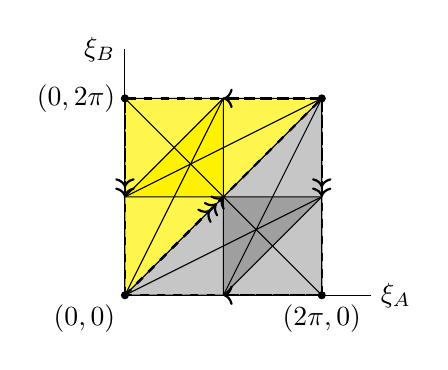
\begin{tikzpicture}
[scale=1.25]
%Points
\filldraw (0,0) circle (1pt); %mid bottom
\filldraw (0,2) circle (1pt); %top left
\filldraw (2,2) circle (1pt); %top right
\filldraw (2,0) circle (1pt); %botom right
%\filldraw (1,1) circle (.5pt); %isosceles point in Q_C
%\filldraw (1,2) circle (.5pt); %isosceles point in Q_C
%\filldraw (0,1) circle (.5pt); %isosceles point in Q_C
%Lines
\draw[thick, dashed] (0,0)--(0,2)--(2,2)--(2,0)--(0,0); %perimeter
\draw[thick, dashed] (0,0)--(2,2); %diagonal
\draw (0,0)--(0,2.5); %y-axis.
\draw (0,0)--(2.5,0); %x-axis.
\draw[thick, dashed, ->] (2,2)--(1,2);
\draw[thick, dashed, ->] (2,0)--(1,0);
\draw[thick, dashed, ->>] (0,2)--(0,1);
\draw[thick, dashed, ->>] (2,2)--(2,1);
\draw[thick, dashed, ->>>] (0,0)--(1,1);
\draw[thin] (0,2)--(2,0); %thin isosceles line
\draw[thin] (0,1)--(2,2); %thin isosceles line
\draw[thin] (0,0)--(1,2); %thin isosceles line
\draw[thin] (0,0)--(2,1);
\draw[thin] (1,0)--(2,2);
%Colors
\begin{scope}[on background layer]
\draw[fill=darkgray!30] (0,0)--(2,2)--(2,0)--(0,0); %lower right
\draw[fill=yellow!70] (0,0)--(2,2)--(0,2)--(0,0); %yellow perimeter
\draw[thin, fill=yellow!100] (1,1)--(1,2)--(0,1)--(1,1); %yellow acute
\draw[thin, fill=darkgray!50] (1,0)--(1,1)--(2,1)--(1,0); %lower right acute
\end{scope}
%Nodes
\node[left] at (0,2) {$(0,2\pi)$};
\node[below] at (2,0) {$(2\pi,0)$};
\node[below left] at (0,0) {$(0,0)$};
\node[right] at (2.5,0) {$\xi_A$};
\node[left] at (0,2.5) {$\xi_B$};
\end{tikzpicture}
\caption{$\sf R/2\pi$ is a Torus} 
\label{fig:R/2pi}
\end{figure}
Thus $\sf{LOT}$ is naturally a topological torus.
\end{proof}

\subsection{Map From Relative Arguments to Angles} %Some text about why this is useful, to introduce it.
We next apply Proposition 20 of 
Euclid III to the plane $\sf R$ of relative arguments $(\xi_A,\xi_B)$ in Figure~\ref{fig:region-r},
to show how even those regions of the plane $A+B+C=\pi$
that are not in the first octant
are identified naturally with positively and negatively oriented triangles,
resulting in a quotient space homeomorphic to the torus of Figure~\ref{fig:R/2pi}.

Denote by $\T_+^\#$ the triangle $\tri((\pi,\pi,-\pi)(-\pi,\pi,\pi)(\pi,-\pi,\pi))$
in Figure \ref{fig:quasi-triangles}.
The triangle of triangles $\T_+$ is the gold-colored subset 
$\tri((\pi,0,0)(0,\pi,0)(0,0,\pi))$.
%Big Triangle of triangles
\begin{figure}[h]
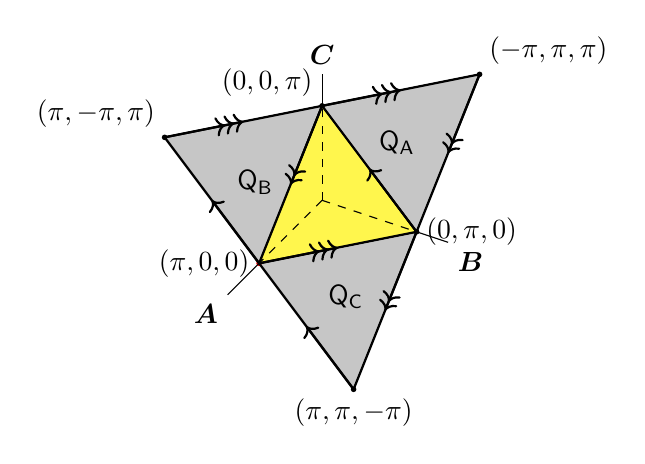
\begin{tikzpicture}[scale=.4]
%Points
\filldraw (0,3) circle (2pt); %top
\filldraw[red] (-2,-2) circle (2pt); %bottom left of OG
\filldraw (3,-1) circle (2pt); %bottom right OG
\filldraw (5,4) circle (2pt); %upper right
\filldraw (-5,2) circle (2pt); %upper left
\filldraw (1,-6) circle (2pt); %bottom
%Lines
\draw[dashed] (0,0) -- (0,3); %z-axis
\draw (0,3) -- (0,4); %top of z-axis
\draw[dashed] (0,0) -- (3,-1); %y-axis
\draw (3,-1) -- (4,-4/3); %end of y-axis
\draw[dashed] (0,0) -- (-2,-2); %x-axis
\draw (-2,-2) -- (-3,-3); %end of x-axis
\draw[thick] (0,3) -- (-2,-2); %left side of OG
\draw[thick] (-2,-2) -- (3,-1); %bottom OG
\draw[thick] (0,3)--(3,-1);
\draw[thick] (5,4)--(-5,2)--(1,-6)--(5,4); %perimeter
\draw[thick, ->] (3,-1)--(1.5,1);
\draw[thick, ->] (-2,-2)--(-3.5,0);
\draw[thick, ->] (1,-6)--(-.5,-4);
\draw[thick, ->>] (0,3)--(-1,.5);
\draw[thick, ->>] (5,4)--(4,1.5);
\draw[thick, ->>] (3,-1)--(2,-3.5);
\draw[thick, ->>>] (-5,2)--(-2.5,2.5);
\draw[thick, ->>>] (0,3)--(2.5,3.5);
\draw[thick, ->>>] (-2,-2)--(.5,-1.5);
%Shading
\begin{scope}[on background layer]
\draw[fill=darkgray!30] (0,3)--(5,4)--(3,-1)--(0,3);
\draw[fill=darkgray!30] (0,3)--(-2,-2)--(-5,2)--(0,3);
\draw[fill=darkgray!30] (-2,-2)--(1,-6)--(3,-1)--(-2,-2);
\draw[fill=yellow!70] (0,3)--(-2,-2)--(3,-1)--(0,3);
\end{scope}
%Nodes
\fill
(0,3) node [above left] {$(0,0,\pi)$}
(3,-1) node [right] {$(0,\pi,0)$}
(-2,-2) node [left] {$(\pi,0,0)$};
\node[above right] at (5,4) {$(-\pi,\pi,\pi)$};
\node[below] at (1,-6) {$(\pi,\pi,-\pi)$};
\node[above left] at (-5,2) {$(\pi,-\pi,\pi)$};
\node[above] at (0,4) {$\boldsymbol C$};
\node[below left] at (-3,-3) {$\boldsymbol A$};
\node[below right] at (4,-4/3) {$\boldsymbol B$};
\node[below left] at (13/4,5/2) {$\sf Q_A$};
\node[below right] at (-3,5/4) {$\sf Q_B$};
\node[above] at (3/4,-15/4) {$\sf Q_C$};
\end{tikzpicture}
\caption{Extended Triangle of Triangles $\T_+^\#$}
\label{fig:quasi-triangles}
\end{figure}

\begin{Theorem}\label{maptoangles}
The linear map 
\[T^\#(\xi_A,\xi_B)\;=\;\left(\pi-\tfrac 12 \xi_B,\,\tfrac 12 \xi_A\,,\tfrac 12(\xi_B-\xi_A)\right)\]
bijects 
$\sf R$ in Figure \ref{fig:region-r} %=\tri((-2\pi,0)(2\pi,0)(2\pi,4\pi))$  
onto 
$\T_+^\#$ in Figure \ref{fig:quasi-triangles}. %=\tri((\pi,\pi,-\pi)(-\pi,\pi,\pi)(\pi,-\pi,\pi))$ 
Explicitly,
let $\sf Q_C,\sf Q_A,\sf Q_C$ be the three gray triangles indicated in Figure \ref{fig:quasi-triangles}.
Then
\[T^\#(\xi_A,\xi_B)\;=\;\begin{cases}
(\alpha,\beta,\gamma)\in\T_+&\text{if $\tri(\xi_A,\xi_B)\in\T_+$}\\
(\pi-\alpha,\pi-\beta,-\gamma)\in\sf Q_C&\text{if $\tri(\xi_A,\xi_B)\in\T_-$ and $\xi_A\geq \xi_B$}\\
(-\alpha,\pi-\beta,\pi-\gamma)\in\sf Q_A&\text{if $\tri(\xi_A,\xi_B)\in\T_-$ and $2\pi\leq \xi_B$}\\
(\pi-\alpha,-\beta,\pi-\gamma)\in\sf Q_B&\text{if $\tri(\xi_A,\xi_B)\in\T_-$ and $\xi_A\leq 0$}\\
\end{cases}
\]
where $0\leq\alpha,\beta,\gamma\leq\pi$ are the non-negative angles
of $\tri(\xi_A,\xi_B)$, 
so $\tri(\xi_A,\xi_B)=(\alpha,\beta,\gamma)$ in $\T_+$
and $\tri(\xi_A,\xi_B)=(-\alpha,-\beta,-\gamma)$ in $\T_-$.
\end{Theorem}

\begin{proof}
Since $T^\#$ is linear and takes the vertices of Figure \ref{fig:region-r} 
to those of Figure \ref{fig:quasi-triangles}, it takes $\sf R$ onto $\T_+^\#$ as stated.
Let $\tri ABC$ be a triangle.
Write $ACB$ for the angle between $0$ and $2\pi$ at $C$ that is on the {\it right} of the directed path $A\to C\to B$.
Then $ACB+BCA=2\pi$ for any triangle $\tri ABC$.

By Euclid (\cite[III Proposition 20]{Euclid}, see also \cite{DJ98}), 
{\it in a circle the angle at the center is double the angle at 
the circumference when the angles have the same circumference as base.}
Thus if $A,B,C$ lie on a circle centered at $O$,
and $BAC\leq\pi$, then $BAC=\frac 12 BOC$, and then $\pi-BAC=\frac 12 COB$ since $2\pi-BOC=COB$.

When $\xi_A\leq \xi_B$, $\tri(\xi_A,\xi_B)$ is positively oriented,
and since $2\pi-\xi_B=BOC$, $\pi-\tfrac 12 \xi_B=\frac 12 BOC$ computes $BAC=\alpha$.
Similarly when $\xi_A\geq \xi_B$, $\tri(\xi_A,\xi_B)$ is negatively oriented,
and $\pi-\tfrac 12 \xi_B=\pi-\tfrac 12 COB$ computes $\pi-CAB=\pi-\alpha$ (see Figure \ref{fig:relatives}).
Applying this reasoning to $\frac 12 \xi_A$ yields $CBA$ and $\pi-ABC$, respectively,
and applying it to $\frac 12(\xi_B-\xi_A)$ yields $BCA$ when $\xi_A\leq \xi_B$, and $\frac 12(\xi_B-\xi_A)=-BCA$
when $\xi_A\geq \xi_B$.
Therefore
\begin{align*}T^\#(\xi_A,\xi_B)
\;&=\;\begin{cases}
(BAC,CBA,ACB)\in\T_+
&\text{when $0\leq \xi_A\leq \xi_B\leq 2\pi$}\\
(\pi-CAB,\pi-ABC,-BCA)\in\sf Q_C %We have to change the order of the angles because now $\xi_A\geq \xi_B$.
&\text{when $\xi_A\geq \xi_B$}\\
(-CAB,\pi-ABC,\pi-BCA)\in\sf Q_A
&\text{when $2\pi\leq \xi_B$}\\
(\pi-CAB,-ABC,\pi-BCA)\in\sf Q_B
&\text{when $\xi_A\leq 0$}
\end{cases}
\end{align*}
This matches the statement of the theorem.
%By definition $CAB$ is the angle between $0$ and $2\pi$ on the right of $C\to A\to B$,
%and the triangle is negatively oriented, so in our notation $CAB=\alpha$ in e.g. case 3.
\end{proof}

\begin{Remark}
Figure \ref{fig:extended-to-negative} shows how $\sf Q_C$
is identified with $\T_-$ via the map $\tri\circ(T^\#)^{-1}$.
\begin{figure}
\centering
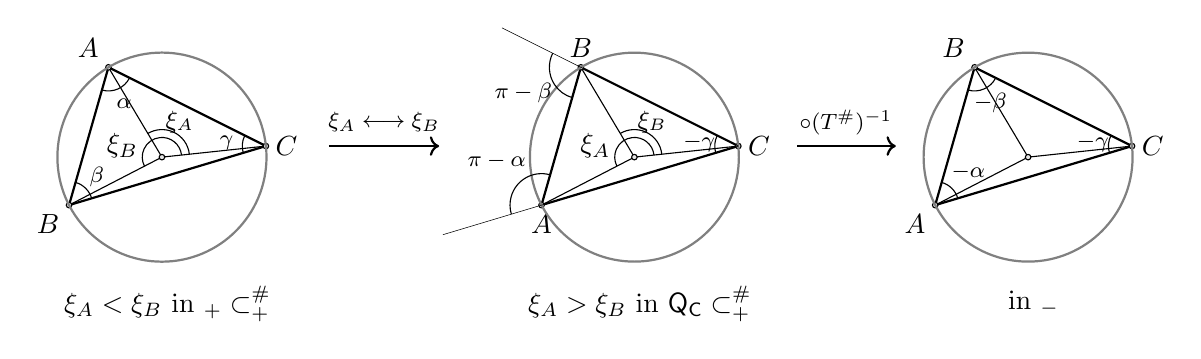
\begin{tikzpicture}
\tkzDefPoints{0/1/A,-.5/-.75/B,2/0/C}
\tkzDrawPolygon[thick](A,B,C)
\tkzDefTriangleCenter[circum](A,B,C)
\tkzGetPoint{O}
%Mark Angles
\tkzMarkAngle[size=.3](B,A,C)
\tkzLabelAngle[pos=.5,font=\footnotesize](B,A,C){$\alpha$}
\tkzMarkAngle[size=.3](A,C,B)
\tkzLabelAngle[pos=.5,font=\footnotesize](A,C,B){$\gamma$}
\tkzMarkAngle[size=.3](C,B,A)
\tkzLabelAngle[pos=.5,font=\footnotesize](C,B,A){$\beta$}
\tkzMarkAngle[size=0.35](C,O,A)
\tkzLabelAngle[pos=0.5,font=\small](C,O,A){$\xi_A$}
\tkzMarkAngle[size=0.25](C,O,B)
\tkzDrawSegments[thin](O,A O,B O,C)
\tkzDrawPoints(A,B,C,O)
\tkzLabelPoints[above left](A)
\tkzLabelPoints[right](C)
\tkzLabelPoints[below left](B)
%\tkzLabelPoints(O)
\tkzDefCircle[circum](A,B,C)
\tkzGetPoint{I}
\tkzDrawCircle[thick](I,A)
%%%%%%%%%%%%%%%%%%%%%%%%%%%%%%%%%%%%%%%%%%%%%
\tkzDefPoints{5.5/-.75/A, 6/1/B,8/0/C}
\tkzDrawPolygon[thick](B,A,C)
\tkzDefTriangleCenter[circum](B,A,C)
\tkzGetPoint{O}
\tkzMarkAngle[size=0.25](C,O,A)
\tkzMarkAngle[size=0.35](C,O,B)
\tkzLabelAngle[pos=0.5,font=\small](C,O,B){$\xi_B$}
\tkzDrawSegments[thin](O,B O,A O,C)
\tkzDrawPoints(B,A,C,O)
\tkzLabelPoints[above](B)
\tkzLabelPoints[right](C)
\tkzLabelPoints[below](A)
%\tkzLabelPoints(O)
\tkzDefCircle[circum](A,B,C)
\tkzGetPoint{I}
\tkzDrawCircle[thick](I,A)
\tkzDrawLines[add=0 and .5](C,B C,A)
%Mark Angles
\tkzMarkAngle[size=.3](B,C,A)
\tkzLabelAngle[pos=0.5,font=\footnotesize](B,C,A){$-\gamma$}
\tkzDefTriangleCenter[ex](B,C,A)
\tkzGetPoint{J_C}
\tkzDefPointBy[projection=onto C--A](J_C)
\tkzGetPoint{D}
\tkzDefPointBy[projection=onto C--B](J_C)
\tkzGetPoint{E}
\tkzMarkAngle[size=.4](B,A,D)
\tkzLabelAngle[pos=0.8,font=\footnotesize](B,A,D){$\pi-\alpha$}
\tkzMarkAngle[size=.4](E,B,A)
\tkzLabelAngle[pos=0.8,font=\footnotesize](E,B,A){$\pi-\beta$}
%%%%%%%%%%%%%%%%%%%%%%%%%%%%%%%%%%%%%%%%%%
\tkzDefPoints{10.5/-.75/A,11/1/B,13/0/C}
\tkzDrawPolygon[thick](A,B,C)
\tkzDefTriangleCenter[circum](A,B,C)
\tkzGetPoint{O}
\tkzDrawSegments[thin](O,B O,A O,C)
\tkzDrawPoints(A,B,C,O)
\tkzLabelPoints[below left](A)
\tkzLabelPoints[right](C)
\tkzLabelPoints[above left](B)
%\tkzLabelPoints(O)
\tkzDefCircle[circum](A,B,C)
\tkzGetPoint{I}
\tkzDrawCircle[thick](I,A)
%Mark Angles
\tkzMarkAngle[size=0.3](A,B,C)
\tkzLabelAngle[pos=0.5,font=\footnotesize](A,B,C){$-\beta$}
\tkzMarkAngle[size=0.3](C,A,B)
\tkzLabelAngle[pos=0.6,font=\footnotesize](C,A,B){$-\alpha$}
\tkzMarkAngle[size=.3](B,C,A)
\tkzLabelAngle[pos=0.5,font=\footnotesize](B,C,A){$-\gamma$}
%Nodes
\node[left] at (.5,0) {$\xi_B$};
\node at (.75,-2) {$\xi_A< \xi_B$ in $\T_+\subset\T_+^\#$};
\node at (3.5,.3) {\footnotesize $\xi_A\longleftrightarrow \xi_B$};
%
\node[left] at (6.5,0) {$\xi_A$};
\node at (6.75,-2) {$\xi_A> \xi_B$ in $\sf Q_C\subset\T_+^\#$};
%
\draw[thick,->] (2.8,0)--(4.2,0);
\node at (9.365,.3) {\footnotesize $\tri\circ(T^\#)^{-1}$};
\draw[thick,->](8.75,0)--(10,0);
\node at (11.75,-2) {in $\T_-$};
\end{tikzpicture}
\caption{Interpretation of $T^\#(\xi_A,\xi_B)$}
\label{fig:extended-to-negative}
\end{figure}
\end{Remark}


Figure \ref{fig:map} is a graphical reprentation of the map $\tri\circ(T^\#)^{-1}$.
\begin{figure}[h]
\centering
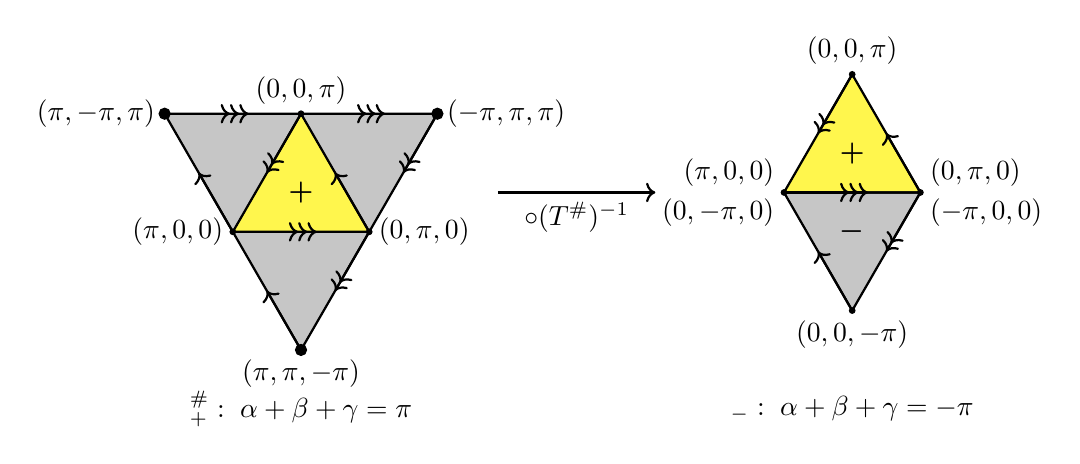
\begin{tikzpicture}[scale=2] %T# and T\sqcup(-T), side by side.
%Points on left side
\filldraw ({3+sqrt(3)/2},1) circle (1pt); %bottom right
\filldraw ({3-sqrt(3)/2},1) circle (1pt); %bottom left
\filldraw (3,-1/2) circle (1pt); %top
\filldraw (3,1) circle (.5pt); %bottom midpoint
\filldraw ({3-sqrt(3)/4},1/4) circle (.5pt);
\filldraw ({3+sqrt(3)/4},1/4) circle (.5pt);
%Lines on left side
\draw[thick, ->] ({3-sqrt(3)/4},1/4)--({3-3*sqrt(3)/8},1/4+3/8); 
\draw[thick, ->] (3,-1/2)--({3-sqrt(3)/8},-1/2+3/8);
\draw[thick, ->] ({3+sqrt(3)/4},1/4)--({3+sqrt(3)/8},1/4+3/8); 
\draw[thick, ->>] (3,1)--({3-sqrt(3)/8},1-3/8); 
\draw[thick, ->>] ({3+sqrt(3)/2},1)--({3+sqrt(3)/2-sqrt(3)/8},1-3/8); 
\draw[thick, ->>] ({3+sqrt(3)/4},1/4)--({3+sqrt(3)/8},1/4-3/8); 
\draw[thick, ->>>] ({3-sqrt(3)/2},1)--({3.1-sqrt(3)/4},1); 
\draw[thick, ->>>] (3,1)--({3.1+sqrt(3)/4},1); 
\draw[thick, ->>>] ({3-sqrt(3)/4},1/4)--(3.1,1/4); 
%More lines on left side
\draw[thick] (3,-1/2)--({3-sqrt(3)/2},1)--({3+sqrt(3)/2},1)--(3,-1/2); %outside triangle
\draw[thick] (3,1)--({3+sqrt(3)/4},1/4)--({3-sqrt(3)/4},1/4)--(3,1); %inside triangle
%shading on left side
\begin{scope}[on background layer]
\draw[fill=yellow!70] (3,1)--({3+sqrt(3)/4},1/4)--({3-sqrt(3)/4},1/4)--(3,1);
\draw[fill=darkgray!30] (3,-1/2)--({3-sqrt(3)/4},1/4)--({3+sqrt(3)/4},1/4)--(3,-1/2); 
\draw[fill=darkgray!30] ({3-sqrt(3)/4},1/4)--({3-sqrt(3)/2},1)--(3,1)--({3-sqrt(3)/4},1/4); 
\draw[fill=darkgray!30] ({3+sqrt(3)/4},1/4)--({3+sqrt(3)/2},1)--(3,1)--({3+sqrt(3)/4},1/4); 
\end{scope}
%nodes on left side
\node[ left] at ({3-sqrt(3)/2},1) {$(\pi,-\pi,\pi)$};
\node[ right] at ({3+sqrt(3)/2},1) {$(-\pi,\pi,\pi)$};
\node[below ] at (3,-1/2) {$(\pi,\pi,-\pi)$};
\node[above] at (3,1) {$(0,0,\pi)$};
\node[left] at ({3-sqrt(3)/4},1/4) {$(\pi,0,0)$};
\node[right] at ({3+sqrt(3)/4},1/4) {$(0,\pi,0)$};
\node at (3,-7/8) {$\T_+^\#:\;\alpha+\beta+\gamma=\pi$};
\node at (3,1/2) {$\boldsymbol +$};
\node[below] at (4.75, .5) {$\tri\circ(T^\#)^{-1}$};
%%%%%%%%%%%%%%%%%%%%%%%%%%%%%%%%%%%%%%%%%%%%%%%%%%%%%%%%%%%%%%%%%%%%%%%%%%%%%%%%%%%%%%%%%%
%%%%%%%%%%%%%%%%%%%%%%%%%%%%%%%%%%%%%%%%%%%%%%%%%%%%%%%%%%%%%%%%%%%%%%%%%%%%%%%%%%%%%%%%%%
%Shadow triangle of triangles:
%Add 3 to the x-component, reverse sign of y-component, add 1/2
%Points on right side
\filldraw (6.5,-1/4) circle (.5pt); %bottom
\filldraw ({6.5-sqrt(3)/4},1/2) circle (.5pt); %left
\filldraw ({6.5+sqrt(3)/4},1/2) circle (.5pt); %right
\filldraw (6.5,5/4) circle (.5pt); %top
%Lines on right side
\draw[thick] (6.5,-1/4)--({6.5+sqrt(3)/4},1/2)--({6.5-sqrt(3)/4},1/2)--(6.5,-1/4); %bottom
\draw[thick] (6.5,5/4) --({6.5+sqrt(3)/4},1/2)--({6.5-sqrt(3)/4},1/2)--(6.5,5/4); %top
\draw[thick, ->] (6.5,-1/4)--({6.5-sqrt(3)/8},1/8); %bottom
\draw[thick, ->>] ({6.5+sqrt(3)/4},1/2)--({6.5+sqrt(3)/8},1/8); %bottom
\draw[thick, ->>>] ({6.5-sqrt(3)/4},1/2)--(6.6,1/2); %middle
\draw[thick, ->] ({6.5+sqrt(3)/4},1/2)--({6.5+sqrt(3)/8},7/8);
\draw[thick, ->>] (6.5,5/4)--({6.5-sqrt(3)/8},7/8); %bottom
%shading on right side
\begin{scope}[on background layer]
\draw[fill=darkgray!30] (6.5,-1/4)--({6.5+sqrt(3)/4},1/2)--({6.5-sqrt(3)/4},1/2)--(6.5,-1/4);
\draw[fill=yellow!70] (6.5,5/4) --({6.5+sqrt(3)/4},1/2)--({6.5-sqrt(3)/4},1/2)--(6.5,5/4);
\end{scope}
%nodes on right side
\node[below] at (6.5,-1/4) {$(0,0,-\pi)$};
\node[left] at ({6.5-sqrt(3)/4},1/2+1/8) {$(\pi,0,0)$};
\node[right] at ({6.5+sqrt(3)/4},1/2+1/8) {$(0,\pi,0)$};
\node at ({6.15-sqrt(3)/4},1/2) {\tiny $\Vvert$};
\node at ({6.85+sqrt(3)/4},1/2) {\tiny $\Vvert$};
\node[left] at ({6.5-sqrt(3)/4},1/2-1/8) {$(0,-\pi,0)$};
\node[right] at ({6.5+sqrt(3)/4},1/2-1/8) {$(-\pi,0,0)$};
\node[above] at (6.5,5/4) {$(0,0,\pi)$};
\node at (6.5,1/4) {$\boldsymbol -$};
\node at (6.5,3/4) {$\boldsymbol +$};
\node at (6.5,-7/8) {$\T_-:\;\alpha+\beta+\gamma=-\pi$};
%%%%%%%%%%%%%%%%%%%%%%%%%%%%%%%%%%%%%%%%%%%%%%%%%%%%%%%%%%%%%%%%%%%%%%%%%%%%%%%%%%%%%%%%%%
%%%%%%%%%%%%%%%%%%%%%%%%%%%%%%%%%%%%%%%%%%%%%%%%%%%%%%%%%%%%%%%%%%%%%%%%%%%%%%%%%%%%%%%%%%
%Line between
\draw[thick,->] (4.25,.5)--(5.25,.5);
\end{tikzpicture}
%\begin{tikzpicture}[scale=1.5]
%\draw[thick] (0,0)--({sqrt(2)},0)--({sqrt(2)/2},1)--(0,0)--({sqrt(2)/2},-1)--({sqrt(2)},0)--(0,0);
%\draw[thick, ->>>](0,0)--({sqrt(2)/2},0);
%\draw[thick, ->]({sqrt(2)},0)--({3*sqrt(2)/4},1/2);
%\draw[thick, ->>]({sqrt(2)/2},1)--({sqrt(2)/4},1/2);
%\draw[thick, ->>]({sqrt(2)},0)--({3*sqrt(2)/4},-1/2);
%\draw[thick, ->]({sqrt(2)/2},-1)--({sqrt(2)/4},-1/2);
%%Shading
%\begin{scope}[on background layer]
%\draw[fill=darkgray!30] (0,0)--({sqrt(2)},0)--({sqrt(2)/2},-1)--(0,0);
%\draw[fill=yellow!70] (0,0)--({sqrt(2)},0)--({sqrt(2)/2},1)--(0,0);
%\end{scope}
%%Nodes
%%\node[left] at (0,0) {$-Q=P$};
%%\node[right] at ({sqrt(2)},0) {$Q=-P$};
%%\node[below] at ({sqrt(2)/2},-1) {$-R$};
%%\node[above] at ({sqrt(2)/2},1) {$R$};
%\end{tikzpicture}
\caption{The Map $\tri\circ(T^\#)^{-1}$}
\label{fig:map}
\end{figure}

\section{\bf Examples of Families}
\label{sec:examples}

Figure \ref{fig:torus-of-t} is an actual torus of triangles, faithfully shaded yellow and gray to represent the positively- 
and negatively-oriented triangles. The degenerate triangles, triangles where a vertex angle is 0, 
are the red curves, tracing the boundaries of the positively- and negatively-oriented regions. 
The isosceles and right families are blue and black, respectively. 
The triple intersection point of the blue isosceles curves in the yellow region 
is the positively-oriented equilateral triangle point; this point has a negatively-oriented counterpart
in the gray region. 
The point shown on the front of the torus in Figure \ref{fig:torus-of-t}, 
where the three red and three blue curves intersect, corresponds to the identified
four corners of the fundamental polygon.

A torus has a nontrivial fundamental group, and therefore ``nontrivial'' loops, not contractible
to a point. 
The families of degenerate, isosceles, and right (oriented labeled) triangles all
determine nontrivial loops. 

\begin{figure}
	\centering
	\includegraphics[width=0.4\textwidth]{pics/torus-right-isosceles-degenerate.png}
	\caption{The Torus of Triangles. Yellow and gray regions represent
	positively- and negatively-oriented triangles, respectively. Black curves are right triangles, 
	blue curves are isosceles, red curves are ``triangles'' with a zero vertex angle.}
	\label{fig:torus-of-t}
\end{figure}

An example of a trivial loop of triangles is shown on the torus in Figure \ref{fig:torus-trivial}, 
and in the $(\xi_A,\xi_B)$-plane in Figure \ref{fig:plane-trivial}. 
These families in the plane are circles, all contractable to the incenter of the right-triangle triangle. 
The actual (3-sided) triangles in this family are illustrated in Figure~\ref{fig:trivial-pencil}. 
A nontrivial family of actual (3-sided) triangles is illustrated in Figure \ref{fig:nontrivial-pencil}. 
This family is generated by fixing vertices $A$ and $B$ and allowing $B$ to wander around the circle. 
Notice how the warm-colored triangles are negatively-oriented and thus located in the gray triangle, 
while the cool-colored triangles are positively-oriented and located in the yellow triangle. 
The yellow triangles in Figure \ref{fig:nontrivial-pencil} are almost degenerate triangles, 
which is seen in Figure \ref{fig:nontrivial-key} 
by the yellow color of the gradient when it cross the diagonal red line which represents degenerate triangles. 

\begin{figure}
\centering
\begin{subfigure}{0.4\textwidth}
	\centering
     \includegraphics[width=0.75\textwidth]{pics/torus-trivial-family.png}
	\caption{A Trivial Family on the Torus.}
	\label{fig:torus-trivial}
\end{subfigure}
\hfill
\begin{subfigure}{0.45\textwidth}
	\centering
    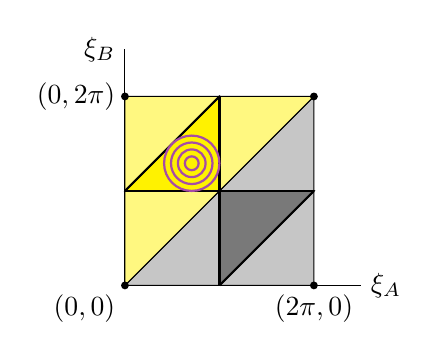
\begin{tikzpicture}[scale=1.2]
%Points
\filldraw (0,0) circle (1pt);
\filldraw (0,2) circle (1pt); %mid left
\filldraw (2,2) circle (1pt); %mid right
\filldraw (2,0) circle (1pt); %lower right
%\filldraw (1,1) circle (.5pt); %isosceles point in Q_C
%\filldraw (1,2) circle (.5pt); %isosceles point in Q_C
%\filldraw (0,1) circle (.5pt); %isosceles point in Q_C
%\filldraw (2/3,4/3) circle (1pt); %equilateral in T
%\draw (2/3,4/3) circle (2pt); %equilateral in T
%\filldraw (4/3,2/3) circle (1pt); %equilateral in Q_C
%\draw (4/3,2/3) circle (2pt); %equilateral in Q_C


\draw (0,0)--(0,2.5); %y-axis.
\draw (0,0)--(2.5,0); %x-axis.

%Lines
%\draw[thick, red] (0,0)--(0,2)--(2,2)--(2,0)--(0,0); %perimeter of OG pic
%\draw[thick, red] (0,0)--(2,2); %diagonal of OG pic
%\draw[thick, dashed] (-2,0)--(2,4)--(2,0)--(-2,0); %perimater of T#
\draw (0,1)--(1,1)--(1,2)--(0,1); %dark yellow triangle
\draw (1,0)--(1,1)--(2,1)--(1,0); %black triangle
% RIGHT
\draw [thick,black] (0,1)--(2,1); %horizontal
\draw [thick,black] (1,0)--(1,2); %vertical
\draw [thick,black] (0,1)--(1,2); %diagonal
\draw [thick,black] (1,0)--(2,1); %diagonal
%ISOSCELES
%\draw [thick, blue](0,2)--(2,0);
%\draw [thick, blue](0,1)--(2,2);
%\draw [thick, blue](0,0)--(2,1);
%\draw [thick, blue](0,0)--(1,2);
%\draw [thick, blue](1,0)--(2,2);


%Colors
\begin{scope}[on background layer]
\draw[fill=darkgray!30] (0,0)--(2,2)--(2,0)--(0,0); %lower right


\draw[fill=yellow!100] (1,1)--(1,2)--(0,1)--(1,1);
\draw[fill=yellow!50] (1,1)--(1,2)--(2,2)--(1,1);
\draw[fill=yellow!50] (1,1)--(0,0)--(0,1)--(1,1);
\draw[fill=yellow!50] (0,1)--(0,2)--(1,2)--(0,1);
\draw[fill=darkgray!70] (1,0)--(1,1)--(2,1)--(1,0); %lower right acute

\end{scope}
%Nodes
\node[left] at (0,2) {$(0,2\pi)$};
\node[below] at (2,0) {$(2\pi,0)$};
\node[below left] at (0,0) {$(0,0)$};
\node[right] at (2.5,0) {$\xi_A$};
\node[left] at (0,2.5) {$\xi_B$};
%\node at (0,-.5) {The region $\sf R$};
% trivial family circle
\tkzDefPoint(sqrt(2)/2,2-sqrt(2)/2){I}
\tkzDefPoint(1,2-sqrt(2)/2){I_1} %largest , 100% radius
\tkzDefPoint(sqrt(2)/8+3/4,2-sqrt(2)/2){I_2} %75% radius
\tkzDefPoint(sqrt(2)/4+1/2,2-sqrt(2)/2){I_3} %50% radius
\tkzDefPoint(3*sqrt(2)/8+1/4,2-sqrt(2)/2){I_4} %25% radius
\tkzDrawCircles[thick,violet!70!white](I,I_1 I,I_2 I,I_3 I,I_4)
\end{tikzpicture}
\caption{A Trivial Family over $\sf R$}
\label{fig:plane-trivial}
\end{subfigure}       
\caption{A Trivial Family}
\label{fig:trivial-family}
\end{figure}

\begin{figure}
\centering
\begin{subfigure}{0.45\textwidth}
\centering
\definecolorseries{first}{rgb}{last}{red}{yellow}
\definecolorseries{second}{rgb}{last}{yellow}{blue}
\definecolorseries{third}{rgb}{last}{blue}{red}
\begin{tikzpicture}[scale=0.75]
	    \def\outRadius{2} % outcircle
	    \def\penRadius{0.75*pi*(1-sqrt(2)/2)} % circle in \xi_A,\xi_B plane
	    \def\xA{pi*(sqrt(2)/2)}
	    \def\yA{pi*(2-(sqrt(2)/2))}
	    \tkzDefPoint(0,0){O}
	    \tkzDefPoint(0:\outRadius){C}
	    
	    \resetcolorseries[15]{first}
	    \foreach \t in {0,0.05,...,0.65}{
	    	\tkzDefPoint(\outRadius*cos(\penRadius*cos(\t*pi)+\xA),\outRadius*sin(\penRadius*cos(\t*pi)+\xA)){A}
	    	\tkzDefPoint(\outRadius*cos(\penRadius*sin(\t*pi)+\yA),\outRadius*sin(\penRadius*sin(\t*pi)+\yA)){B}
	     \draw [very thick,color=first!!+](A) -- (B) -- (C) -- (A);
		}
		\resetcolorseries[15]{second}
        \foreach \t in {0.65,0.7,...,1.35}{
	    	\tkzDefPoint(\outRadius*cos(\penRadius*cos(\t*pi)+\xA),\outRadius*sin(\penRadius*cos(\t*pi)+\xA)){A}
	    	\tkzDefPoint(\outRadius*cos(\penRadius*sin(\t*pi)+\yA),\outRadius*sin(\penRadius*sin(\t*pi)+\yA)){B}
	     \draw [very thick,color=second!!+](A) -- (B) -- (C) -- (A);
		}
		\resetcolorseries[15]{third}
        \foreach \t in {1.35,1.4,...,2}{
	    	\tkzDefPoint(\outRadius*cos(\penRadius*cos(\t*pi)+\xA),\outRadius*sin(\penRadius*cos(\t*pi)+\xA)){A}
	    	\tkzDefPoint(\outRadius*cos(\penRadius*sin(\t*pi)+\yA),\outRadius*sin(\penRadius*sin(\t*pi)+\yA)){B}
	     \draw [very thick,color=third!!+](A) -- (B) -- (C) -- (A);
		}
		% special triangle
		\def\arg{0.75} %make sure to change for other figure as well
		\tkzDefPoint(\outRadius*cos(\penRadius*cos(\arg*pi)+\xA),\outRadius*sin(\penRadius*cos(\arg*pi)+\xA)){A}
	    \tkzDefPoint(\outRadius*cos(\penRadius*sin(\arg*pi)+\yA),\outRadius*sin(\penRadius*sin(\arg*pi)+\yA)){B}
	    \draw [ultra thick,black](A) -- (B) -- (C) -- (A);
	    \tkzDrawCircle[very thick, black](O,C)
	    \tkzDrawPoints[ultra thick, black](A,B,C)
	    \tkzLabelPoint[above](A){$A(\xi_A)$}
	    \tkzLabelPoint[below](B){$B(\xi_B)$}
	    \tkzLabelPoint[right](C){$C$}
\end{tikzpicture}
\caption{The Triangles in a Trivial Family.}
\label{fig:trivial-pencil}
\end{subfigure}
\hfill
\begin{subfigure}{0.45\textwidth}
\centering
\begin{tikzpicture}[scale=1.2]
\begin{scope}[on background layer]
\draw[fill=darkgray!30] (0,0)--(2,2)--(2,0)--(0,0); %lower right


\draw[fill=yellow!70] (1,1)--(1,2)--(0,1)--(1,1);
\draw[fill=yellow!30] (1,1)--(1,2)--(2,2)--(1,1);
\draw[fill=yellow!30] (1,1)--(0,0)--(0,1)--(1,1);
\draw[fill=yellow!30] (0,1)--(0,2)--(1,2)--(0,1);
\draw[fill=darkgray!70] (1,0)--(1,1)--(2,1)--(1,0); %lower right acute
 \end{scope}
%Points
\filldraw (0,0) circle (1pt);
\filldraw (0,2) circle (1pt); %mid left
\filldraw (2,2) circle (1pt); %mid right
\filldraw (2,0) circle (1pt); %lower right
\filldraw (1,1) circle (.5pt); %isosceles point in Q_C
\filldraw (1,2) circle (.5pt); %isosceles point in Q_C
\filldraw (0,1) circle (.5pt); %isosceles point in Q_C
% \filldraw (2/3,4/3) circle (1pt); %equilateral in T
% \draw (2/3,4/3) circle (2pt); %equilateral in T
% \filldraw (4/3,2/3) circle (1pt); %equilateral in Q_C
% \draw (4/3,2/3) circle (2pt); %equilateral in Q_C


\draw (0,0)--(0,2.5); %y-axis.
\draw (0,0)--(2.5,0); %x-axis.

%Lines
%\draw[red,thick] (0,0)--(0,2)--(2,2)--(2,0)--(0,0); %perimeter of OG pic
%\draw[red,thick] (0,0)--(2,2); %diagonal of OG pic
%\draw[thick, dashed] (-2,0)--(2,4)--(2,0)--(-2,0); %perimater of T#
\draw (0,1)--(1,1)--(1,2)--(0,1); %dark yellow triangle
\draw (1,0)--(1,1)--(2,1)--(1,0); %black triangle
% RIGHT
\draw [black] (0,1)--(2,1); %horizontal
\draw [black] (1,0)--(1,2); %vertical
\draw [black] (0,1)--(1,2); %diagonal
\draw [black] (1,0)--(2,1); %diagonal
%ISOSCELES
\draw [black](0,2)--(2,0);
\draw [black](0,1)--(2,2);
\draw [black](0,0)--(2,1);
\draw [black](0,0)--(1,2);
\draw [black](1,0)--(2,2);


%Colors

%Nodes
\node[left] at (0,2) {$(0,2\pi)$};
\node[below] at (2,0) {$(2\pi,0)$};
\node[below left] at (0,0) {$(0,0)$};
\node[right] at (2.5,0) {$\xi_A$};
\node[left] at (0,2.5) {$\xi_B$};
%\node at (0,-.5) {The region $\sf R$};
% trivial family circle
\tkzDefPoint(sqrt(2)/2,2-sqrt(2)/2){I}
\tkzDefPoint(1,2-sqrt(2)/2){I_1} %largest , 100% radius
% \tkzDefPoint(sqrt(2)/8+3/4,2-sqrt(2)/2){I_2} %75% radius
% \tkzDefPoint(sqrt(2)/4+1/2,2-sqrt(2)/2){I_3} %50% radius
% \tkzDefPoint(3*sqrt(2)/8+1/4,2-sqrt(2)/2){I_4} %25% radius
\tkzCalcLength(I,I_1)\tkzGetLength{radius}
\resetcolorseries[360]{first}
\foreach \t in {0,0.01,...,0.7}{
    \tkzDefPoint(0.75*(1-(sqrt(2)/2))*cos(\t*pi)+(sqrt(2)/2),0.75*(1-(sqrt(2)/2))*sin(\t*pi)+(2-sqrt(2)/2)){P}
    \tkzDrawPoint[thin, color=first!!+](P)
}
\resetcolorseries[330]{second}
\foreach \t in {0.71,0.72,...,1.35}{
    \tkzDefPoint(0.75*(1-(sqrt(2)/2))*cos(\t*pi)+(sqrt(2)/2),0.75*(1-(sqrt(2)/2))*sin(\t*pi)+(2-sqrt(2)/2)){P}
    \tkzDrawPoint[thin, color=second!!+](P)
}
\resetcolorseries[330]{third}
\foreach \t in {1.36,1.37,...,2}{
    \tkzDefPoint(0.75*(1-(sqrt(2)/2))*cos(\t*pi)+(sqrt(2)/2),0.75*(1-(sqrt(2)/2))*sin(\t*pi)+(2-sqrt(2)/2)){P}
    \tkzDrawPoint[thin, color=third!!+](P)
}
% special black dot
\def\arg{0.75}
\tkzDefPoint(0.75*(1-(sqrt(2)/2))*cos(\arg*pi)+(sqrt(2)/2),0.75*(1-(sqrt(2)/2))*sin(\arg*pi)+(2-sqrt(2)/2)){T}
\tkzDrawPoint[black, thick](T)
\tkzLabelPoint[left](T){$\triangle{ABC}$}

\end{tikzpicture}
\caption{Triangles in the Region $\sf R$}
\label{fig:trivial-key}
\end{subfigure}
\caption{The Triangles in a Trivial Family. Point $\triangle{ABC}$ in Figure \ref{fig:trivial-key} represents $\triangle{ABC}$ in Figure \ref{fig:trivial-family}.}
\label{fig:trivial}
\end{figure}

\begin{figure}
\centering
\begin{subfigure}{0.45\textwidth}
\centering
\definecolorseries{first}{rgb}{last}{red}{yellow}
\definecolorseries{second}{rgb}{last}{yellow}{blue}
\definecolorseries{third}{rgb}{last}{blue}{red}
\begin{tikzpicture}[scale=0.75]
	    \def\outRadius{2} % outcircle
	    \tkzDefPoint(0,0){O}
	    \tkzDefPoint(0:\outRadius){C}
	    \tkzDefPoint(120: \outRadius){A}
	    \resetcolorseries[13]{first}
	    \foreach \t in {0,10,...,120}{
	    	\tkzDefPoint(\t:\outRadius){B}
	     \draw [very thick,color=first!!+](A) -- (B) -- (C) -- (A);
		}
 		\resetcolorseries[13]{second}
        \foreach \t in {120,130,...,240}{
	    	\tkzDefPoint(\t:\outRadius){B}
	     \draw [very thick,color=second!!+](A) -- (B) -- (C) -- (A);
		}
 		\resetcolorseries[13]{third}
        \foreach \t in {250,260,...,350}{
	    	\tkzDefPoint(\t:\outRadius){B}
	     \draw [very thick,color=third!!+](A) -- (B) -- (C) -- (A);
		}
		% special triangle
		\def\arg{240} %make sure to change for other figure as well
	    \tkzDefPoint(\arg:\outRadius){B}
	    \draw [ultra thick,black](A) -- (B) -- (C) -- (A);
	    \tkzDrawCircle[very thick, black](O,C)
	    \tkzDrawPoints[ultra thick, black](A,B,C)
	    \tkzLabelPoint[above](A){$A$}
	    \tkzLabelPoint[below](B){$B(\xi_B)$}
	    \tkzLabelPoint[right](C){$C$}
\end{tikzpicture}
\caption{The Triangles in a Nontrivial Family.}
\label{fig:nontrivial-pencil}
\end{subfigure}
\hfill
\begin{subfigure}{0.45\textwidth}
\centering
\begin{tikzpicture}[scale=1.2]
\begin{scope}[on background layer]
\draw[fill=darkgray!30] (0,0)--(2,2)--(2,0)--(0,0); %lower right


\draw[fill=yellow!70] (1,1)--(1,2)--(0,1)--(1,1);
\draw[fill=yellow!30] (1,1)--(1,2)--(2,2)--(1,1);
\draw[fill=yellow!30] (1,1)--(0,0)--(0,1)--(1,1);
\draw[fill=yellow!30] (0,1)--(0,2)--(1,2)--(0,1);
\draw[fill=darkgray!70] (1,0)--(1,1)--(2,1)--(1,0); %lower right acute
 \end{scope}
%Points
\filldraw (0,0) circle (1pt);
\filldraw (0,2) circle (1pt); %mid left
\filldraw (2,2) circle (1pt); %mid right
\filldraw (2,0) circle (1pt); %lower right
\filldraw (1,1) circle (.5pt); %isosceles point in Q_C
\filldraw (1,2) circle (.5pt); %isosceles point in Q_C
\filldraw (0,1) circle (.5pt); %isosceles point in Q_C
% \filldraw (2/3,4/3) circle (1pt); %equilateral in T
% \draw (2/3,4/3) circle (2pt); %equilateral in T
% \filldraw (4/3,2/3) circle (1pt); %equilateral in Q_C
% \draw (4/3,2/3) circle (2pt); %equilateral in Q_C


\draw (0,0)--(0,2.5); %y-axis.
\draw (0,0)--(2.5,0); %x-axis.

%Lines
%\draw[red,thick] (0,0)--(0,2)--(2,2)--(2,0)--(0,0); %perimeter of OG pic
%\draw[red,thick] (0,0)--(2,2); %diagonal of OG pic
%\draw[thick, dashed] (-2,0)--(2,4)--(2,0)--(-2,0); %perimater of T#
\draw (0,1)--(1,1)--(1,2)--(0,1); %dark yellow triangle
\draw (1,0)--(1,1)--(2,1)--(1,0); %black triangle
% RIGHT
\draw [black] (0,1)--(2,1); %horizontal
\draw [black] (1,0)--(1,2); %vertical
\draw [black] (0,1)--(1,2); %diagonal
\draw [black] (1,0)--(2,1); %diagonal
%ISOSCELES
\draw [black](0,2)--(2,0);
\draw [black](0,1)--(2,2);
\draw [black](0,0)--(2,1);
\draw [black](0,0)--(1,2);
\draw [black](1,0)--(2,2);


%Colors

%Nodes
\node[left] at (0,2) {$(0,2\pi)$};
\node[below] at (2,0) {$(2\pi,0)$};
\node[below left] at (0,0) {$(0,0)$};
\node[right] at (2.5,0) {$\xi_A$};
\node[left] at (0,2.5) {$\xi_B$};
%\node at (0,-.5) {The region $\sf R$};
% trivial family circle
\resetcolorseries[360]{first}
\foreach \t in {0,0.01,...,0.7}{
    \tkzDefPoint(2/3, \t){P}
    \tkzDrawPoint[thin, color=first!!+](P)
}
\resetcolorseries[330]{second}
\foreach \t in {0.71,0.72,...,1.35}{
    \tkzDefPoint(2/3, \t){P}
    \tkzDrawPoint[thin, color=second!!+](P)
}
\resetcolorseries[330]{third}
\foreach \t in {1.36,1.37,...,2}{
    \tkzDefPoint(2/3, \t){P}
    \tkzDrawPoint[thin, color=third!!+](P)
}
% special black dot
\def\arg{4/3}
\tkzDefPoint(2/3,\arg){T}
\tkzDrawPoint[black, thick](T)
\tkzLabelPoint[left](T){$\triangle{ABC}$}


\end{tikzpicture}
\caption{Nontrivial Triangles in the Region $\sf R$}
\label{fig:nontrivial-key}
\end{subfigure}
\caption{The Triangles in a Nontrivial Family. Point $\triangle{ABC}$ in Figure \ref{fig:nontrivial-key} represents $\triangle{ABC}$, the equilateral triangle, in Figure \ref{fig:nontrivial-pencil}.}
\label{fig:nontrivial}
\end{figure}


\begin{Remark}
If $\sf R$ is replaced by the entire $(\xi_A,\xi_B)$-plane then $T^\#$ maps
to the entire plane $A+B+C=\pi$, and partitions it into up-triangles, 
which we would color in gold,
and down-triangles, which we would put in gray. 
The resulting map $\tri\circ T^\#$ to the torus $\T_+\cup(\T_-)$ yields
an interpretation of every point in the plane as a positively or negatively oriented labeled triangle.
\end{Remark} 

\clearpage
\bibliographystyle{alpha} %other choices are plain or abbrv or alpha
\bibliography{../../mathdocs.bib}

\end{document}

%Map from $R/2\pi$ to Triples of Angles.

\begin{figure}
\centering
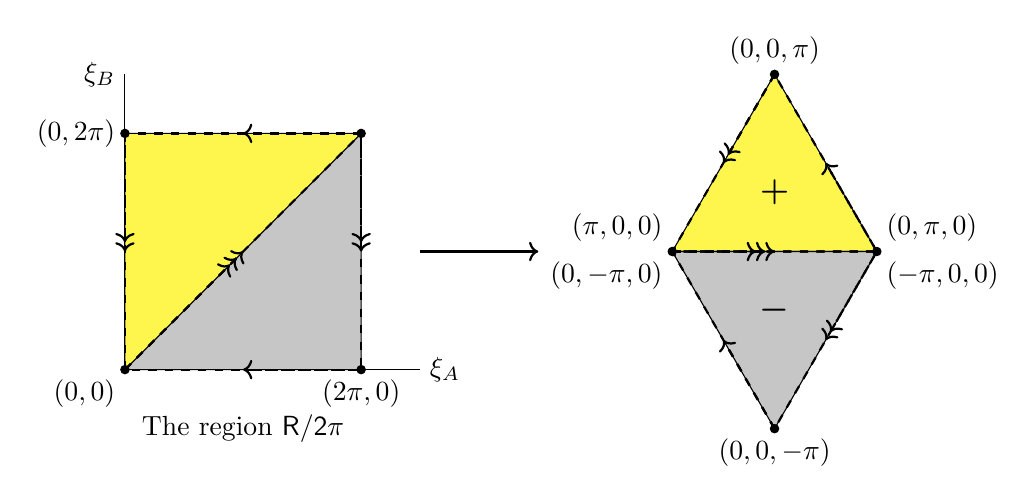
\begin{tikzpicture}[scale=1.5]
%Points
\filldraw (0,0) circle (1pt); %mid bottom
\filldraw (0,2) circle (1pt); %top left
\filldraw (2,2) circle (1pt); %top right
\filldraw (2,0) circle (1pt); %botom right
%\filldraw (1,1) circle (.5pt); %isosceles point in Q_C
%\filldraw (1,2) circle (.5pt); %isosceles point in Q_C
%\filldraw (0,1) circle (.5pt); %isosceles point in Q_C
%Lines
\draw[thick, dashed] (0,0)--(0,2)--(2,2)--(2,0)--(0,0); %perimeter
\draw[thick, dashed] (0,0)--(2,2); %diagonal
\draw (0,0)--(0,2.5); %y-axis.
\draw (0,0)--(2.5,0); %x-axis.
\draw[thick, dashed, ->] (2,2)--(1,2);
\draw[thick, dashed, ->] (2,0)--(1,0);
\draw[thick, dashed, ->>] (0,2)--(0,1);
\draw[thick, dashed, ->>] (2,2)--(2,1);
\draw[thick, dashed, ->>>] (0,0)--(1,1);
\draw[thick, ->] (2.5,1)--(3.5,1);
%Colors
\begin{scope}[on background layer]
\draw[fill=darkgray!30] (0,0)--(2,2)--(2,0)--(0,0); %lower right
\draw[fill=yellow!70] (0,0)--(2,2)--(0,2)--(0,0); %yellow perimeter
%\draw[fill=yellow!100] (1,1)--(1,2)--(0,1)--(1,1); %yellow acute
%\draw[fill=darkgray!50] (1,0)--(1,1)--(2,1)--(1,0); %lower right acute
\end{scope}
%Nodes
\node[left] at (0,2) {$(0,2\pi)$};
\node[below] at (2,0) {$(2\pi,0)$};
\node[below left] at (0,0) {$(0,0)$};
\node[right] at (2.5,0) {$\xi_A$};
\node[left] at (0,2.5) {$\xi_B$};
\node at (1,-.5) {The region $\sf R/2\pi$};
%%%%%%%%%%%%%%%%%%%%%%%%%%%%%%%%%%%%%%%%%%%%%%%%%%%%
%Points
\filldraw ({5.5+sqrt(3)/2},1) circle (1pt); % right
\filldraw ({5.5+-sqrt(3)/2},1) circle (1pt); % left
\filldraw (5.5,5/2) circle (1pt); %top gold
%\filldraw (5.5,1) circle (.5pt); %bottom foot gold
%\filldraw ({5.5-sqrt(3)/4},7/4) circle (.5pt); %left foot gold
%\filldraw ({5.5+sqrt(3)/4},7/4) circle (.5pt); %right foot gold
%\filldraw ({5.5-sqrt(3)/4},1/4) circle (.5pt); %left foot gray
%\filldraw ({5.5+sqrt(3)/4},1/4) circle (.5pt); %right foot gray
\filldraw (5.5,-1/2) circle (1pt); %bottom gray
%Lines
\draw[thick,dashed] (5.5,5/2)--({5.5-sqrt(3)/2},1)--({5.5+sqrt(3)/2},1)--(5.5,5/2); %perimeter gold triangle
%\draw (5.5,1)--({5.5+sqrt(3)/4},7/4)--({5.5-sqrt(3)/4},7/4)--(5.5,1); %perimeter dark gold
\draw[thick,dashed] (5.5,-1/2)--({5.5-sqrt(3)/2},1)--({5.5+sqrt(3)/2},1)--(5.5,-1/2); %perimater gray
%\draw (5.5,1)--({5.5+sqrt(3)/4},1/4)--({5.5-sqrt(3)/4},1/4)--(5.5,1); %perimeter dark gray
\draw[thick,dashed,->>] (5.5,5/2)--({5.5-sqrt(3)/4},7/4); %gold
\draw[thick,dashed,->>>] ({5.5-sqrt(3)/2},1)--(5.5,1); %gold
\draw[thick,dashed,->] ({5.5+sqrt(3)/2},1)--({5.5+sqrt(3)/4},7/4); %gold
\draw[thick,dashed,->] (5.5,-1/2)--({5.5-sqrt(3)/4},1/4); %gray
\draw[thick,dashed,->>] ({5.5+sqrt(3)/2},1)--({5.5+sqrt(3)/4},1/4);
%Shading
\begin{scope}[on background layer]
%\draw[fill=yellow!100] (5.5,1)--({5.5+sqrt(3)/4},7/4)--({5.5-sqrt(3)/4},7/4)--(5.5,1);
\draw[fill=yellow!70] (5.5,5/2)--({5.5-sqrt(3)/2},1)--({5.5+sqrt(3)/2},1)--(5.5,5/2); 
\draw[fill=darkgray!30] (5.5,-1/2)--({5.5-sqrt(3)/2},1)--({5.5+sqrt(3)/2},1)--(5.5,-1/2);
%\draw[fill=darkgray!50] (5.5,1)--({5.5+sqrt(3)/4},1/4)--({5.5-sqrt(3)/4},1/4)--(5.5,1);
\end{scope}
%nodes
\node[above left] at ({5.5-sqrt(3)/2},1) {$(\pi,0,0)$};
\node[below left] at ({5.5-sqrt(3)/2},1) {$(0,-\pi,0)$};
\node[above right] at ({5.5+sqrt(3)/2},1) {$(0,\pi,0)$};
\node[below right] at ({5.5+sqrt(3)/2},1) {$(-\pi,0,0)$};
\node[above ] at (5.5,5/2) {$(0,0,\pi)$};
\node[below] at (5.5,-1/2) {$(0,0,-\pi)$};
\node at (5.5,1/2) {\large$\boldsymbol -$};
\node at (5.5,3/2) {\large $\boldsymbol +$};
\end{tikzpicture}
\caption{Pairs of Arguments vs. Triples of Angles} 
\label{fig:R/2pi}
\end{figure}